\documentclass[a4paper,10pt,oneside]{amsart}
\usepackage[a4paper,textwidth=15.5cm]{geometry}
\usepackage{amsmath,amsthm,amssymb,amsfonts}
\usepackage[dvipsnames]{xcolor}
% Palette from the diagrams in Acyclic_Maps_and_the_Plus_Construction.
\definecolor{AcyclicPink}{RGB}{214,92,92}
\definecolor{AcyclicBlue}{RGB}{92,92,214}
\definecolor{AcyclicGrey}{RGB}{153,153,153}
\usepackage{tikz-cd}
% The built-in preview does not include quiver.sty; the styles used by these exports are included below.
% Curve style from quiver.sty, due to Andr\'eC: https://github.com/varkor/quiver/blob/master/package/quiver.sty.
\usetikzlibrary{calc}
\tikzset{
  2tail reversed/.code={\pgfsetarrowsstart{Implies}},
  curve/.style={settings={#1},to path={
    (\tikztostart)
    .. controls ($(\tikztostart)!\pv{pos}!(\tikztotarget)!\pv{height}!270:(\tikztotarget)$)
    and ($(\tikztostart)!1-\pv{pos}!(\tikztotarget)!\pv{height}!270:(\tikztotarget)$)
    .. (\tikztotarget)\tikztonodes
  }},
  settings/.code={\tikzset{quiver/.cd,#1}\def\pv##1{\pgfkeysvalueof{/tikz/quiver/##1}}},
  quiver/.cd,pos/.initial=0.35,height/.initial=0
}
\usepackage[backref=page]{hyperref}
\hypersetup{colorlinks=true,linkcolor=AcyclicBlue,citecolor=AcyclicPink,urlcolor=AcyclicBlue}
\renewcommand{\sectionautorefname}{Section}
\renewcommand{\subsectionautorefname}{Section}
\usepackage{thmtools}

% Commutative diagrams were imported and exported through https://q.uiver.app on 2026-10-29.
% Each diagram has an editable quiver URL; manuscript spacing is retained where specified.
% Typography and theorem style follow the acyclic maps project with Giacomo.
% Faithful transcription of the handwritten notes, with approved corrections.
% Mathematical corrections were approved by the author on 2026-10-28; the prose was subsequently revised at the author's request.
% Shared numbering with distinct reference names for each environment.
\declaretheorem[style=definition,numberwithin=section,name=Theorem]{theorem}
\declaretheorem[style=definition,sibling=theorem,name=Definition]{definition}
\declaretheorem[style=definition,sibling=theorem,name=Proposition]{proposition}
\declaretheorem[style=definition,sibling=theorem,name=Corollary]{corollary}
\declaretheorem[style=definition,sibling=theorem,name=Lemma]{lemma}
\declaretheorem[style=definition,sibling=theorem,name=Remark]{remark}
\declaretheorem[style=definition,sibling=theorem,name=Example]{example}
\declaretheorem[style=definition,sibling=theorem,name=Conjecture]{conjecture}

\title{Group Cohomology\\[0.6em]
{\footnotesize From a geometric point of view}}
\date{}

\begin{document}
% Course attribution verified against the University of Regensburg catalogue:
% https://hellus.app.uni-regensburg.de/KVV/abruflink.php?id=1135
\begin{abstract}
These are lecture notes for the course on group cohomology given by Kevin Li at the University of Regensburg during the winter semester 2023--2024.
\end{abstract}
\maketitle
\tableofcontents
\clearpage

\section{Motivations}
\label{sec:motivations}
% Source: handwritten PDF, page 3.
This course concerns the relation between two notions of dimension for groups.
We begin with the geometric notion.
Let $X$ be a CW-complex equipped with a filtration
\[
\varnothing=X^{(-1)}\subseteq X^{(0)}\subseteq X^{(1)}\subseteq\cdots\subseteq\bigcup_{n\in\mathbb{N}}X^{(n)}=X.
\]
Recall that this means that the $n$-skeleton $X^{(n)}$ of $X$ is constructed by attaching $n$-cells to $X^{(n-1)}$ via a pushout
\[
% https://q.uiver.app/#q=WzAsNCxbMCwwLCJcXGNvcHJvZF97XFxhbHBoYVxcaW4gQX1TXntuLTF9Il0sWzEsMCwiWF57KG4tMSl9Il0sWzAsMSwiXFxjb3Byb2Rfe1xcYWxwaGFcXGluIEF9RF5uIl0sWzEsMSwiWF57KG4pfSJdLFswLDFdLFswLDJdLFswLDMsIlxcbWF0aHJteyhwbyl9IiwxLHsic3R5bGUiOnsiYm9keSI6eyJuYW1lIjoibm9uZSJ9LCJoZWFkIjp7Im5hbWUiOiJub25lIn19fV0sWzEsM10sWzIsM11d
\begin{tikzcd}
	{\coprod_{\alpha\in A}S^{n-1}} & {X^{(n-1)}} \\
	{\coprod_{\alpha\in A}D^n} & {X^{(n)}}
	\arrow[from=1-1, to=1-2]
	\arrow[from=1-1, to=2-1]
	\arrow["{\mathrm{(po)}}"{description}, draw=none, from=1-1, to=2-2]
	\arrow[from=1-2, to=2-2]
	\arrow[from=2-1, to=2-2]
\end{tikzcd}
\]
% Approved correction: S^{n-1} replaces the apparent S^n in the source.
and that the topology on $X$ is the weak one ($A\subseteq X$ is closed $\Leftrightarrow A\cap X^{(n)}$ is closed for every $n\in\mathbb{N}$).
The dimension of a CW-complex records the highest dimension in which cells occur.
\begin{definition}
\label{def:geometric-dimension-space}
Let $X$ be a CW-complex.
We define its \emph{geometric dimension} to be
\[
\operatorname{gd}(X)=\inf\{n\in\mathbb{N}\mid X=X^{(n)}\}.
\]
\end{definition}
The value $\operatorname{gd}(X)$ lies in $\mathbb{N}\cup\{\infty\}$ and is infinite when $X$ has cells in arbitrarily high dimensions.
If $\operatorname{gd}(X)<\infty$, we say that $X$ is \emph{finite-dimensional}.
We can also consider the number of cells in each dimension.
Geometric dimension records the dimensions of the cells, but not their number.
We say that $X$ has a \emph{finite $n$-skeleton} if it has finitely many cells in dimensions at most $n$.
\begin{example}
The CW-complex $\bigvee_{\mathbb{N}}S^1$ has dimension $1$ and infinitely many $1$-cells.
Conversely, $\mathbb{RP}^{\infty}=\bigcup_{n\in\mathbb{N}}\mathbb{RP}^n$ has one cell in each dimension, but has infinite dimension.
\end{example}

% Source: handwritten PDF, page 4.
We now relate these notions to groups.
\begin{definition}
\label{def:classifying-space-intro}
Let $G$ be a discrete group and let $X$ be a connected CW-complex with a basepoint $x\in X$.
We say that $X$ is a \emph{model for $BG=K(G,1)$} if $\pi_1(X,x)\cong G$ and the universal cover of $X$ is contractible (that is, $\pi_n(X,x)\cong 0$ for $n\geq 2$).
\end{definition}
As we will see in \autoref{subsec:topological-resolutions}, a model for $BG$ exists and is unique up to homotopy equivalence.
The uniqueness follows from \autoref{prop:classifying-space-universal-property} and \autoref{thm:whitehead}.
\begin{example}
A model for $B\mathbb{Z}$ is given by $S^1$, since $\pi_1(S^1)\cong\mathbb{Z}$ and the universal cover $\mathbb{R}\to S^1$ is contractible.
Similarly, a model for $B(\mathbb{Z}\times\mathbb{Z})$ is given by the torus $T_1$.
% Blue annotation in the source.
Categorically, this also follows from the adjunction
\[
\pi_1:h\mathrm{CW}_*\rightleftarrows\mathrm{Grp}:B
\]
between $\pi_1$ and the $B$-construction.
Here $h\mathrm{CW}_*$ denotes the homotopy category of pointed connected CW-complexes, with pointed homotopy classes of maps.
This follows from the universal property in \autoref{prop:classifying-space-universal-property}.
% Audit correction approved by the author: specify connected pointed spaces and use the proved universal property instead of the unexplained Brown-representability attribution.
\end{example}
\begin{example}
A model for $B(\mathbb{Z}*\mathbb{Z})$ is $S^1\vee S^1$: its fundamental group is $\mathbb{Z}*\mathbb{Z}$, and its universal cover is the contractible Cayley tree on two generators.
% Approved replacement of the pink annotation, which claimed that a right adjoint preserves colimits.
The functor $B$ is a right adjoint and preserves products.
The wedge example follows from \autoref{lem:classifying-space-amalgam}.
\end{example}
\begin{example}
Do we have a model for $B\mathbb{Z}/2$?
We have $\pi_1(\mathbb{RP}^2)\cong\mathbb{Z}/2$, but the universal cover $S^2\to\mathbb{RP}^2$ is not contractible, so $\mathbb{RP}^2$ is not a model for $B(\mathbb{Z}/2)$.
In \autoref{ex:classifying-spaces} we will see that $\mathbb{RP}^{\infty}\simeq B(\mathbb{Z}/2\mathbb{Z})$, since $S^{\infty}\to\mathbb{RP}^{\infty}$ is a universal cover.
\end{example}
The dimension of a CW-model for $BG$ leads to the following definition.
% Source: handwritten PDF, page 5.
\begin{definition}
\label{def:geometric-dimension-group}
Let $G$ be a discrete group.
The \emph{geometric dimension} of $G$ is
\[
\operatorname{gd}(G)=\inf\{n\in\mathbb{N}\mid\text{there exists a model of }BG\text{ of dimension }n\}.
\]
\end{definition}
% Approved correction: ``least'' replaces ``greatest''.
To compute the geometric dimension of $G$, we take the least dimension among all CW-models for $BG$.
\begin{example}
Let us compute $\operatorname{gd}(\mathbb{Z}\times\mathbb{Z})$.
We know that $T_1$ is a model for $B(\mathbb{Z}\times\mathbb{Z})$, and that it has dimension $2$, giving us $\operatorname{gd}(\mathbb{Z}\times\mathbb{Z})\leq 2$.
Can $\operatorname{gd}(\mathbb{Z}\times\mathbb{Z})$ be $1$?
% Approved wording adjustment: ``since'' replaces the prohibited causal conjunction.
If so, then $\pi_1(S^1\times S^1)$ would be free, since the fundamental group of a connected one-dimensional CW-complex is free.
This is impossible, so $\operatorname{gd}(\mathbb{Z}\times\mathbb{Z})=2$.
\end{example}
\begin{example}
Let us compute $\operatorname{gd}(\mathbb{Z}/2)$.
The space $\mathbb{RP}^{\infty}$ is a model for $B(\mathbb{Z}/2)$ and has nonzero cohomology in arbitrarily high degrees.
% Approved correction: ``finite-dimensional'' replaces ``finite''.
Since no finite-dimensional CW-complex has this property, we must have $\operatorname{gd}(\mathbb{Z}/2)=\infty$.
\end{example}
This first notion of dimension is geometric.
We next introduce a notion whose algebraic nature will become clear from the construction of group cohomology.
\begin{definition}
\label{def:cohomological-dimension}
Let $G$ be a discrete group and let $BG$ be a CW-model for its classifying space.
We define the \emph{cohomological dimension} to be
\[
\operatorname{cd}(G)=\sup\{n\in\mathbb{N}\mid H^n(BG;M)\neq 0\text{ for }M\in {}_G\mathrm{Mod}\}.
\]
Here $M$ ranges over left $G$-modules, and $H^n(BG;M)$ is cohomology with the associated local coefficients, as in \autoref{def:twisted-cohomology}.
\end{definition}
We will explain this definition in \autoref{subsec:topological-resolutions}; for now, note the inequality of \autoref{thm:cd-le-gd}
\[
\operatorname{cd}(G)\leq\operatorname{gd}(G)
\]
which expresses the possibility that algebraic invariants do not fully determine geometric dimension.

The following theorem shows how closely the two dimensions are related.
% Source: handwritten PDF, page 6.
% Approved correction: omit the incomplete year in the handwritten attribution.
A reference for this theorem is \cite[Theorem~F.3.2]{Dav08}.
\begin{theorem}[Eilenberg--Ganea]
\label{thm:eilenberg-ganea}
Let $G$ be a discrete group.
We have $\operatorname{gd}(G)\leq\max(\operatorname{cd}(G),3)$.
\end{theorem}
Thus, if $\operatorname{cd}(G)\geq 3$, then $\operatorname{cd}(G)=\operatorname{gd}(G)$.
We prove \autoref{thm:eilenberg-ganea} in \autoref{thm:eilenberg-ganea-bound}.
It remains to study the cases where $\operatorname{cd}(G)<3$.
For $\operatorname{cd}(G)=1$ we have an answer, which we will not prove.
% Approved correction: Stallings--Swan; omit the incomplete year.
See \cite[Theorem~F.3.3]{Dav08}.
\begin{theorem}[Stallings--Swan]
\label{thm:stallings-swan}
Let $G$ be a discrete group.
If $\operatorname{cd}(G)=1$, then $G$ is a free group.
\end{theorem}
Indeed, if $\operatorname{cd}(G)=1$, then \autoref{thm:stallings-swan} gives $G\cong\mathrm{Free}(S)$ for some set $S$.
Thus a model for $BG$ is the one-point union $\bigvee_S S^1$ of copies of $S^1$ indexed by $S$, giving us $\operatorname{gd}(G)=1$.
Hence the remaining case is $\operatorname{cd}(G)=2$.
The assertion that the two dimensions also agree in this case is the Eilenberg--Ganea conjecture.
\begin{conjecture}[Eilenberg--Ganea, 1957]
\label{conj:eilenberg-ganea}
Let $G$ be a discrete group with $\operatorname{cd}(G)=2$.
Then $\operatorname{gd}(G)=2$.
\end{conjecture}
The conjecture was open when this course was given in the winter semester 2023--2024.
It was subsequently disproved in the September 2026 OpenAI preprint~\cite{OAI26}.
The counterexample is a finitely generated residually finite group $G$ satisfying
\[
\operatorname{cd}(G)=2,\qquad \operatorname{gd}(G)=3.
\]
% Editorial update requested by the author on 2026-10-29: state the conjecture and its disproof in the introduction.
% The scope of the accompanying Lean formalization is described at https://github.com/openai/math/blob/main/lean/docs/249.md.
We will discuss proposed examples in \autoref{subsec:virtual-dimension} and \autoref{subsec:exotic-finiteness}.
We will also study finiteness conditions.
These concern the number of cells in each skeleton of a CW-complex.
The first such condition is the following.
\begin{definition}
\label{def:type-fn}
Let $G$ be a discrete group and let $n\geq 0$ be an integer.
We say that $G$ is of \emph{type $F_n$} if there exists a model for $BG$ with finite $n$-skeleton.
\end{definition}
These conditions reflect familiar group properties.
For example, a group $G$ is of type $F_1$ if and only if it is finitely generated, and of type $F_2$ if and only if it is finitely presented.
As with dimension, these geometric conditions have algebraic counterparts.
% Source: handwritten PDF, page 7, ending before Homological algebra.
\begin{definition}
\label{def:type-fpn}
Let $G$ be a discrete group and let $n\geq 0$ be an integer.
% Approved clarification: Z is the trivial ZG-module.
We say that $G$ is of \emph{type $\mathrm{FP}_n$} if there exists a projective resolution $P_\bullet\to\mathbb{Z}\to 0$ of the trivial $\mathbb{Z}G$-module $\mathbb{Z}$ in which $P_i$ is finitely generated as a $G$-module for every $0\leq i\leq n$.
\end{definition}
One can show that type $F_n\Rightarrow$ type $\mathrm{FP}_n$.
Does the converse also hold?
Actually, it does not.
The examples are due to Bestvina and Brady~\cite[Examples~6.3(3)]{BB97}.
\begin{theorem}[Bestvina--Brady]
\label{thm:bestvina-brady}
For every integer $n\geq 2$, there exists a discrete group $G$ of type $\mathrm{FP}_n$ but not of type $F_n$.
\end{theorem}
This follows from \autoref{ex:bestvina-brady-acyclic}, using \autoref{thm:bestvina-brady-finiteness}.

\section{Definition of group cohomology}
\label{sec:definition-group-cohomology}
\subsection{Group rings and cohomology}
\label{subsec:group-rings}
% Source: handwritten PDF, page 8 (originally numbered 1.1).
\begin{definition}
\label{def:group-ring}
Let $G$ be a discrete group.
The \emph{group ring} $\mathbb{Z}G$ has the free abelian group on $G$ as its underlying additive group, with multiplication extending the group operation linearly.
\end{definition}
More explicitly, the elements of $\mathbb{Z}G$ are formal sums $\sum_{g\in G}n_g\cdot g$ with $n_g\in\mathbb{Z}$, all but finitely many of which are zero.
Addition is defined coefficientwise, and multiplication extends the group operation linearly.
The ring $\mathbb{Z}G$ is unital, with unit $e_G$, and is commutative if and only if $G$ is abelian.
\begin{example}
Let us see some examples.
If $G=\{e_G\}$ is the trivial group, then $\mathbb{Z}\{e_G\}\cong\mathbb{Z}$ via $e_G\mapsto 1$.
\end{example}
\begin{example}
If $G=\mathbb{Z}$ is the group of integers, then $\mathbb{Z}G\cong\mathbb{Z}[T,T^{-1}]$ is the ring of Laurent polynomials.
Writing $G=\langle t\rangle$, we obtain the isomorphism
\[
\sum_{n\in\mathbb{Z}}a_nt^n\mapsto\sum_{n\in\mathbb{Z}}a_nT^n,
\]
where only finitely many $a_n$ are nonzero.
% Audit clarification approved by the author: distinguish group elements from coefficients and extend the map linearly.
In a similar way, if $n\geq 1$ is an integer and $G=\mathbb{Z}/n\mathbb{Z}$, then $\mathbb{Z}G\cong\mathbb{Z}[T]/(T^n-1)$.
\end{example}
The group ring construction extends to a functor $\mathbb{Z}:\mathrm{Grp}\to\mathrm{Ring}$.
Indeed, every group homomorphism $\varphi:G\to H$ extends linearly to a ring homomorphism $\mathbb{Z}\varphi:\mathbb{Z}G\to\mathbb{Z}H$.
The inclusion $G\hookrightarrow\mathbb{Z}G$, given by $g\mapsto g$, lands in the group of units $(\mathbb{Z}G)^\times$, since every $g\in G$ is invertible.
This is an instance of the following universal property.
% Approved correction: the extension has codomain R, not its group of units.
% The triangle is a diagram of sets, not a diagram in the category of groups.
\begin{proposition}
\label{prop:group-ring-universal-property}
Let $G$ be a discrete group, let $R$ be a unital ring, not necessarily commutative, and let $f:G\to R^\times$ be a group homomorphism.
Then there exists a unique unital ring homomorphism $\overline{f}:\mathbb{Z}G\to R$ such that
\[
% https://q.uiver.app/#q=WzAsNCxbMCwwLCJHIl0sWzEsMCwiUl5cXHRpbWVzIl0sWzAsMSwiXFxtYXRoYmJ7Wn1HIl0sWzEsMSwiUiJdLFswLDEsImYiXSxbMCwyLCIiLDAseyJzdHlsZSI6eyJ0YWlsIjp7Im5hbWUiOiJob29rIiwic2lkZSI6InRvcCJ9fX1dLFsxLDMsIiIsMCx7InN0eWxlIjp7InRhaWwiOnsibmFtZSI6Imhvb2siLCJzaWRlIjoidG9wIn19fV0sWzIsMywiXFxvdmVybGluZXtmfSIsMix7InN0eWxlIjp7ImJvZHkiOnsibmFtZSI6ImRhc2hlZCJ9fX1dXQ==
\begin{tikzcd}
	G & {R^\times} \\
	{\mathbb{Z}G} & R
	\arrow["f", from=1-1, to=1-2]
	\arrow[hook, from=1-1, to=2-1]
	\arrow[hook, from=1-2, to=2-2]
	\arrow["{\overline{f}}"', dashed, from=2-1, to=2-2]
\end{tikzcd}
\]
commutes as a diagram of sets.
\end{proposition}
% Source: handwritten PDF, page 9.
\begin{proof}
Given $f:G\to R^\times$, its unique linear extension is
\[
\overline{f}\left(\sum_{g\in G}n_g\cdot g\right):=\sum_{g\in G}n_g f(g).
\]
Since $f$ is a group homomorphism, $\overline{f}$ is clearly a ring map.
\end{proof}
By using \autoref{prop:group-ring-universal-property}, we get a bijection
\[
\operatorname{Hom}_{\mathrm{Ring}}(\mathbb{Z}G,R)\cong\operatorname{Hom}_{\mathrm{Grp}}(G,R^\times)
\]
for every group $G$ and ring $R$.
Hence we have an adjunction
\[
\mathbb{Z}:\mathrm{Grp}\rightleftarrows\mathrm{Ring}:(-)^\times,
\]
where the unit is a monomorphism.
\begin{remark}
We can also form group rings with coefficients in another ring.
% Approved correction: R is commutative for this formulation with R-algebras.
Categorically, for every commutative unital ring $R$ we get an adjunction
\[
R[-]:\mathrm{Grp}\rightleftarrows R\mathrm{Alg}:(-)^\times
\]
where $R[-]$ sends a group to its group ring over $R$, by the same construction.
\end{remark}
We now consider modules over $\mathbb{Z}G$.
Throughout, rings need not be commutative, and modules are left modules unless stated otherwise.
We will denote by ${}_G\mathrm{Mod}$ the category of left $\mathbb{Z}G$-modules, and call it the category of left $G$-modules.
Equivalently, a $G$-module is an abelian group with a compatible $G$-action.
More precisely, we use the following definition.
\begin{definition}
\label{def:group-module}
Let $G$ be a discrete group.
A \emph{$G$-module} is an abelian group $A$ with an action $G\times A\to A$ such that
\begin{enumerate}
\item $e_G\cdot a=a$ for every $a\in A$;
\item $g\cdot(a+b)=g\cdot a+g\cdot b$ for every $a,b\in A$ and $g\in G$;
\item $h\cdot(g\cdot a)=(hg)\cdot a$ for every $a\in A$ and $g,h\in G$.
\end{enumerate}
\end{definition}
Every abelian group can be given the trivial $G$-action.
This defines a functor ${}_{\mathbb{Z}}\mathrm{Mod}\to {}_G\mathrm{Mod}$, sending an abelian group to the same group with trivial action.
\begin{example}
\label{ex:trivial-module-projective}
Let $G$ be a discrete group.
The trivial $G$-module $\mathbb{Z}$ will be central to \autoref{def:group-cohomology}.
% Source: handwritten PDF, page 10.
The module structure of $\mathbb{Z}$ already detects a property of $G$.
We claim that $\mathbb{Z}$ is projective as a $G$-module if and only if $G=\{1\}$.
The reverse implication is immediate; for the forward implication, suppose that $\mathbb{Z}$ is projective and $G\neq\{1\}$.
Then the lifting problem
\[
% https://q.uiver.app/#q=WzAsNCxbMSwwLCJcXG1hdGhiYntafSJdLFswLDEsIlxcbWF0aGJie1p9RyJdLFsxLDEsIlxcbWF0aGJie1p9Il0sWzIsMSwiMCJdLFswLDIsIlxcbWF0aHJte2lkfSJdLFswLDEsIlxcd2lkZXRpbGRle1xcbWF0aHJte2lkfX0iLDIseyJzdHlsZSI6eyJib2R5Ijp7Im5hbWUiOiJkYXNoZWQifX19XSxbMSwyLCJcXHZhcmVwc2lsb24iLDJdLFsyLDNdXQ==
\begin{tikzcd}
	& {\mathbb{Z}} & \\
	{\mathbb{Z}G} & {\mathbb{Z}} & 0
	\arrow["{\widetilde{\mathrm{id}}}"', dashed, from=1-2, to=2-1]
	\arrow["{\mathrm{id}}", from=1-2, to=2-2]
	\arrow["\varepsilon"', from=2-1, to=2-2]
	\arrow[from=2-2, to=2-3]
\end{tikzcd}
\qquad (\text{where }\varepsilon:g\mapsto 1)
\]
has a solution $\widetilde{\mathrm{id}}$.
Since $\mathbb{Z}$ has a trivial $G$-action, $\widetilde{\mathrm{id}}$ must land in $(\mathbb{Z}G)^G$.
By \autoref{lem:group-ring-invariants}, if $|G|=\infty$, then $(\mathbb{Z}G)^G=0$, so $\widetilde{\mathrm{id}}=0$, a contradiction.
If $G$ is finite, then \autoref{lem:group-ring-invariants} gives $(\mathbb{Z}G)^G=\langle N\rangle$ for $N=\sum_{g\in G}g$.
Then $\widetilde{\mathrm{id}}(1)=aN$ for some $a\in\mathbb{Z}$.
Thus $\varepsilon(\widetilde{\mathrm{id}}(1))=a|G|=1$, forcing $|G|=1$.
\end{example}
\begin{example}
\label{ex:permutation-modules}
Let $G$ be a discrete group.
$\mathbb{Z}G$ is a free $G$-module.
More generally, let $S$ be a $G$-set.
Then the action of $G$ on the basis $S$ makes $\mathbb{Z}[S]:=\bigoplus_{s\in S}\mathbb{Z}\cdot s$ a $G$-module, and if $S$ is a free $G$-set, then $\mathbb{Z}[S]$ is a free $G$-module.
Indeed, $S=\coprod_{S/G}G$ can be written in terms of its orbits and $\mathbb{Z}(\coprod_{S/G}G)\cong\bigoplus_{S/G}\mathbb{Z}G$, since $\mathbb{Z}[-]$ is a left adjoint.
% Approved clarification of the sentence about cosets: the construction always applies, but freeness requires H to be trivial.
The construction applies in particular to $S=G/H$, the set of cosets of $H\leq G$.
The freeness assertion applies to this $G$-set only when $H$ is trivial.
\end{example}
\begin{example}
\label{ex:universal-cover-chains}
Consider a connected CW-complex $X$ with fundamental group $G$, and let $\widetilde{X}$ be its universal cover.
Let $n\geq 0$ be an integer.
The group $G$ acts freely on $\widetilde X$, hence also on its $n$-cells and singular $n$-simplices.
These actions make $C_n^{\mathrm{cell}}(\widetilde X;\mathbb{Z})$ and $C_n^{\mathrm{sing}}(\widetilde X;\mathbb{Z})$ free $G$-modules.
\end{example}
Having introduced $G$-modules and seen some examples, we can give the definition of group cohomology.
\begin{definition}
\label{def:group-cohomology}
Let $G$ be a discrete group and let $M$ be a left $G$-module.
The \emph{group cohomology} of $G$ with values in $M$ is
\[
H^\bullet(G,M)=\operatorname{Ext}_{\mathbb{Z}G}^\bullet(\mathbb{Z},M)
\]
in nonnegative degrees, where $\mathbb{Z}$ is the trivial $G$-module.
\end{definition}
% Source: handwritten PDF, page 11.
Note that
\[
H^n(\{1\},M)=\operatorname{Ext}_{\mathbb{Z}}^n(\mathbb{Z},M)\cong
\begin{cases}
M & \text{for }n=0,\\
0 & \text{for }n\neq 0.
\end{cases}
\]
The degree-zero derived functor gives the following result.
\begin{lemma}
\label{lem:degree-zero-invariants}
Let $G$ be a discrete group and let $M$ be a left $G$-module.
Then $H^0(G,M)\cong M^G$, where $M^G=\{m\in M\mid gm=m\text{ for every }g\in G\}$.
\end{lemma}
\begin{proof}
The degree-zero derived functor is naturally isomorphic to the original left exact functor.
Hence $H^0(G,M)=\operatorname{Hom}_{\mathbb{Z}G}(\mathbb{Z},M)$.
It therefore suffices to construct a natural isomorphism $\operatorname{Hom}_{\mathbb{Z}G}(\mathbb{Z},-)\cong(-)^G$.
To do that, define
\[
\begin{aligned}
\varphi_M:\operatorname{Hom}_{\mathbb{Z}G}(\mathbb{Z},M)&\to M^G\\
(f:\mathbb{Z}\to M)&\mapsto f(1).
\end{aligned}
\]
\end{proof}
Using \autoref{lem:degree-zero-invariants}, the following computation gives the degree-zero cohomology of $\mathbb{Z}G$.
\begin{lemma}
\label{lem:group-ring-invariants}
Let $G$ be a discrete group, and equip $\mathbb{Z}G$ with the left $G$-action by left multiplication.
Then
\[
(\mathbb{Z}G)^G\cong
\begin{cases}
0 & \text{if }G\text{ is infinite},\\
\mathbb{Z} & \text{if }G\text{ is finite}.
\end{cases}
\]
More precisely, if $G$ is finite, we define the \emph{norm element}
\[
N=\sum_{g\in G}1\cdot g\in\mathbb{Z}G,
\]
% Approved correction: add the missing invariants superscript.
and $(\mathbb{Z}G)^G=\langle N\rangle$.
\end{lemma}
\begin{proof}
\begin{enumerate}
\item Assume $|G|=\infty$.
Then $a\in(\mathbb{Z}G)^G$ if and only if $g\cdot a=a$ for every $g\in G$.
Write $a=\sum_{h\in G}n_h\cdot h$ as a finite linear combination.
Then $ga=a$ implies that
\[
g\cdot a=\sum_{h\in G}n_h\cdot gh=\sum_{h'\in G}n_{h'}\cdot h'=a,
\]
Thus $n_h=n_{gh}$ for every $g,h\in G$, so all coefficients agree.
Since $G$ is infinite and $a$ has finite support, these coefficients are zero.
\item Assume that $G$ is finite.
We show that $(\mathbb{Z}G)^G=\mathbb{Z}\langle N\rangle$.
First of all, $g\cdot N=\sum_{h\in G}g\cdot h=\sum_{h\in G}h$ since $G$ is finite.
Moreover, if $a\in(\mathbb{Z}G)^G$, then by writing $a=\sum_{h\in G}n_h\cdot h$ we have that $g\cdot a=\sum_{h\in G}n_h\cdot gh=\sum_{h'\in G}n_{h'}h'=a$.
% Source: handwritten PDF, page 12.
This implies that $n_h=n_{gh}$, which means that all coefficients are the same; hence $a=n\cdot N$.
\end{enumerate}
\end{proof}
By \autoref{lem:degree-zero-invariants} and \autoref{lem:group-ring-invariants} we have that
\[
G\text{ is infinite}\Leftrightarrow H^0(G;\mathbb{Z}G)=0.
\]
This illustrates the dependence of cohomology on the coefficient module.
To compute $H^\bullet(G;M)=\operatorname{Ext}_{\mathbb{Z}G}^\bullet(\mathbb{Z},M)$, we choose a projective resolution of the trivial $\mathbb{Z}G$-module $\mathbb{Z}$.
We begin with a surjection onto $\mathbb{Z}$.
We have a canonical choice:
\begin{definition}
\label{def:augmentation-map}
Let $G$ be a discrete group, equip $\mathbb{Z}G$ with its left multiplication action, and equip $\mathbb{Z}$ with the trivial $G$-action.
The \emph{augmentation map} $\varepsilon:\mathbb{Z}G\to\mathbb{Z}$ is defined by $g\mapsto 1$.
\end{definition}
Clearly, the augmentation map is a surjective $G$-homomorphism.
To extend this to a projective resolution of $\mathbb{Z}$, we consider its kernel
\[
0\to IG\to\mathbb{Z}G\xrightarrow{\varepsilon}\mathbb{Z}\to 0
\]
which in general is not projective.
We have the following description of this kernel.
\begin{lemma}
\label{lem:augmentation-ideal-generators}
Let $G$ be a discrete group and let $IG=\ker(\varepsilon:\mathbb{Z}G\to\mathbb{Z})$, where $\varepsilon$ is the augmentation map of \autoref{def:augmentation-map}.
We regard $IG$ as a left $G$-module by left multiplication.
\begin{enumerate}
\item $IG$ is generated, as an abelian group, by $\{g-1\in\mathbb{Z}G\mid g\in G\}$.
Here $1$ is the unit of $\mathbb{Z}G$.
\item Let $S\subseteq G$ be a subset.
Then $S$ generates $G$ if and only if $\{s-1\mid s\in S\}$ generates $IG$ as a $G$-module.
\item The group $G$ is finitely generated if and only if $IG$ is finitely generated as a $G$-module.
\end{enumerate}
\end{lemma}
\begin{proof}
\begin{enumerate}
\item First of all, $g-1\in IG$ for every $g\in G$.
Let $x=\sum n_g\cdot g\in IG=\ker(\varepsilon)$.
Then $\sum n_g=0$ and so
\[
x=x-0=\sum n_g\cdot g-\sum n_g\cdot 1=\sum n_g\cdot(g-1).
\]
\item $(\Rightarrow)$ If $S$ generates $G$, we want to show that $g-1=\sum\lambda_s(s-1)$ for $\lambda_s\in\mathbb{Z}G$.
Allowing inverses of elements of $S$, we write
% Source: handwritten PDF, page 13.
% Approved correction: restore the missing -1 after the product.
\[
g-1=s_1\cdots s_k-1=(s_1\cdots s_{k-1})(s_k-1)+\cdots
\]
as a telescoping sum.
% Yellow annotation in the source.
Note that $s^{-1}-1=-s^{-1}(s-1)$.
$(\Leftarrow)$ Let $H=\langle S\rangle\leq G$.
We show $H=G$.
Consider the basis element $eH\in\mathbb{Z}[G/H]$.
Now for all $s\in S$
\[
(s-1)\cdot eH=sH-eH=eH-eH=0
\]
since $s\in H$.
As $IG$ is generated by the elements $s-1$, we obtain $(IG)\cdot eH=0$.
Thus $(g-1)eH=0$ for every $g\in G$, so $gH=H$ and hence $g\in H$.
\item It follows from (2).
% Pink annotation in the source.
The reverse implication requires a little care.
\end{enumerate}
\end{proof}
% Approved explanatory comment, supplementing the handwritten pink annotation.
% If x_1,...,x_r generate IG as a G-module, write each x_i as a finite
% integer linear combination of g-1, using (1).
% The union S of the finitely many group elements occurring is finite.
% The G-submodule generated by {s-1 : s in S} contains all x_i, so it is IG.
% Assertion (2) then shows that S generates G.
For more explicit computations, we now specialize to cyclic groups.

\subsection{Cohomology of cyclic groups}
\label{subsec:cyclic-groups}
% Source: handwritten PDF, page 13, originally subsection 1.2.
We begin by looking at the case of cyclic groups $G=\langle t\rangle$.
In this case, \autoref{lem:augmentation-ideal-generators}(2) ensures that $IG$ is generated, as a $G$-module, by one element.
Hence we can continue our sequence as
\[
% https://q.uiver.app/#q=WzAsNSxbMCwwLCJcXG1hdGhiYntafUciXSxbMiwwLCJcXG1hdGhiYntafUciXSxbMywwLCJcXG1hdGhiYntafSJdLFs0LDAsIjAiXSxbMSwxLCJJRz0odC0xKSJdLFswLDEsIi1cXGNkb3QodC0xKSIsMCx7InN0eWxlIjp7ImJvZHkiOnsibmFtZSI6ImRhc2hlZCJ9fX1dLFswLDQsIiIsMCx7InN0eWxlIjp7ImhlYWQiOnsibmFtZSI6ImVwaSJ9fX1dLFsxLDIsIlxcdmFyZXBzaWxvbiJdLFsyLDNdLFs0LDEsIiIsMCx7InN0eWxlIjp7InRhaWwiOnsibmFtZSI6Imhvb2siLCJzaWRlIjoidG9wIn19fV1d
\begin{tikzcd}
	{\mathbb{Z}G} && {\mathbb{Z}G} & {\mathbb{Z}} & 0 \\
	& {IG=(t-1)}
	\arrow["{-\cdot(t-1)}", dashed, from=1-1, to=1-3]
	\arrow[two heads, from=1-1, to=2-2]
	\arrow["\varepsilon", from=1-3, to=1-4]
	\arrow[from=1-4, to=1-5]
	\arrow[hook, from=2-2, to=1-3]
\end{tikzcd}
\]
which is clearly exact.
To go further, we need to compute
\[
\ker(-\cdot(t-1))=(\mathbb{Z}G)^G.
\]

We distinguish two cases using \autoref{lem:group-ring-invariants}.
If $G\cong\mathbb{Z}$ is infinite cyclic, then $(\mathbb{Z}G)^G\cong 0$, and so
\[
% https://q.uiver.app/#q=WzAsNSxbMCwwLCIwIl0sWzEsMCwiXFxtYXRoYmJ7Wn1bXFxtYXRoYmJ7Wn1dIl0sWzIsMCwiXFxtYXRoYmJ7Wn1bXFxtYXRoYmJ7Wn1dIl0sWzMsMCwiXFxtYXRoYmJ7Wn0iXSxbNCwwLCIwIl0sWzAsMV0sWzEsMiwiLVxcY2RvdCh0LTEpIl0sWzIsMywiXFx2YXJlcHNpbG9uIl0sWzMsNF1d
\begin{tikzcd}
	0 & {\mathbb{Z}[\mathbb{Z}]} & {\mathbb{Z}[\mathbb{Z}]} & {\mathbb{Z}} & 0
	\arrow[from=1-1, to=1-2]
	\arrow["{-\cdot(t-1)}", from=1-2, to=1-3]
	\arrow["\varepsilon", from=1-3, to=1-4]
	\arrow[from=1-4, to=1-5]
\end{tikzcd}
\]
is the short exact sequence of $\mathbb{Z}[\mathbb{Z}]$-modules we were looking for.
Hence, for every $M\in {}_{\mathbb{Z}[\mathbb{Z}]}\mathrm{Mod}$ we have
% Approved correction: use the unaugmented cochain complex with the correct Hom arguments.
\[
% https://q.uiver.app/#q=WzAsNixbMCwwLCIwIl0sWzEsMCwiXFxvcGVyYXRvcm5hbWV7SG9tfV97XFxtYXRoYmJ7Wn1bXFxtYXRoYmJ7Wn1dfShcXG1hdGhiYntafVtcXG1hdGhiYntafV0sTSkiXSxbMiwwLCJcXG9wZXJhdG9ybmFtZXtIb219X3tcXG1hdGhiYntafVtcXG1hdGhiYntafV19KFxcbWF0aGJie1p9W1xcbWF0aGJie1p9XSxNKSJdLFszLDAsIjAiXSxbMSwxLCJNIl0sWzIsMSwiTSJdLFswLDFdLFsxLDIsInQtMSJdLFsxLDQsIlxcY29uZyIsMSx7InN0eWxlIjp7ImJvZHkiOnsibmFtZSI6Im5vbmUifSwiaGVhZCI6eyJuYW1lIjoibm9uZSJ9fX1dLFsyLDNdLFsyLDUsIlxcY29uZyIsMSx7InN0eWxlIjp7ImJvZHkiOnsibmFtZSI6Im5vbmUifSwiaGVhZCI6eyJuYW1lIjoibm9uZSJ9fX1dXQ==
\begin{tikzcd}[column sep=small]
	0 & {\operatorname{Hom}_{\mathbb{Z}[\mathbb{Z}]}(\mathbb{Z}[\mathbb{Z}],M)} & {\operatorname{Hom}_{\mathbb{Z}[\mathbb{Z}]}(\mathbb{Z}[\mathbb{Z}],M)} & 0 \\
	& M & M
	\arrow[from=1-1, to=1-2]
	\arrow["{t-1}", from=1-2, to=1-3]
	\arrow["\cong"{description}, draw=none, from=1-2, to=2-2]
	\arrow[from=1-3, to=1-4]
	\arrow["\cong"{description}, draw=none, from=1-3, to=2-3]
\end{tikzcd}
\]
giving us
\[
H^\bullet(\mathbb{Z};M)\cong
\begin{cases}
M^{\mathbb{Z}} & \bullet=0,\\
M_{\mathbb{Z}} & \bullet=1,\\
0 & \bullet\neq 0,1.
\end{cases}
\]
% Blue annotation in the source.
Here $M_{\mathbb{Z}}$ denotes the coinvariants.
In particular, note that the group cohomology
\[
H^\bullet(\mathbb{Z};\mathbb{Z})\cong\mathbb{Z}\cdot 0\oplus\mathbb{Z}\cdot 1+0
\]
is identical to the integral cohomology $H^\bullet(S^1;\mathbb{Z})$ of $S^1$.
% Source: handwritten PDF, page 14.
The topological interpretation in \autoref{subsec:topological-resolutions} explains this agreement.
The second case is when $G\cong\mathbb{Z}/n$ is a finite cyclic group.
In this case \autoref{lem:group-ring-invariants} implies that
\[
% https://q.uiver.app/#q=WzAsOCxbMCwwLCJcXG1hdGhiYntafVtHXSJdLFsxLDAsIlxcbWF0aGJie1p9W0ddIl0sWzIsMCwiXFxtYXRoYmJ7Wn1bR10iXSxbMywwLCJcXG1hdGhiYntafVtHXSJdLFs0LDAsIlxcbWF0aGJie1p9Il0sWzUsMCwiMCJdLFsyLDEsIihcXG1hdGhiYntafUcpXkdcXGNvbmdcXG1hdGhiYntafVxcbGFuZ2xlIE5cXHJhbmdsZSJdLFszLDEsIklHPSh0LTEpIl0sWzAsMSwiLVxcY2RvdCh0LTEpIl0sWzEsMiwiLVxcY2RvdCBOIiwwLHsic3R5bGUiOnsiYm9keSI6eyJuYW1lIjoiZGFzaGVkIn19fV0sWzEsNiwiIiwwLHsic3R5bGUiOnsiaGVhZCI6eyJuYW1lIjoiZXBpIn19fV0sWzIsMywiLVxcY2RvdCh0LTEpIl0sWzIsNywiIiwwLHsic3R5bGUiOnsiaGVhZCI6eyJuYW1lIjoiZXBpIn19fV0sWzMsNCwiXFx2YXJlcHNpbG9uIl0sWzQsNV0sWzYsMiwiIiwwLHsic3R5bGUiOnsidGFpbCI6eyJuYW1lIjoiaG9vayIsInNpZGUiOiJ0b3AifX19XSxbNywzLCIiLDAseyJzdHlsZSI6eyJ0YWlsIjp7Im5hbWUiOiJob29rIiwic2lkZSI6InRvcCJ9fX1dXQ==
\begin{tikzcd}[column sep=small]
	{\mathbb{Z}[G]} & {\mathbb{Z}[G]} & {\mathbb{Z}[G]} & {\mathbb{Z}[G]} & {\mathbb{Z}} & 0 \\
	&& {(\mathbb{Z}G)^G\cong\mathbb{Z}\langle N\rangle} & {IG=(t-1)}
	\arrow["{-\cdot(t-1)}", from=1-1, to=1-2]
	\arrow["{-\cdot N}", dashed, from=1-2, to=1-3]
	\arrow[two heads, from=1-2, to=2-3]
	\arrow["{-\cdot(t-1)}", from=1-3, to=1-4]
	\arrow[two heads, from=1-3, to=2-4]
	\arrow["\varepsilon", from=1-4, to=1-5]
	\arrow[from=1-5, to=1-6]
	\arrow[hook, from=2-3, to=1-3]
	\arrow[hook, from=2-4, to=1-4]
\end{tikzcd}
\]
since $\ker(-\cdot(t-1))=(\mathbb{Z}G)^G\cong\mathbb{Z}\langle N\rangle$ is generated by the norm element.
By going further, we have
\[
\ker(-\cdot N)=\cdots=\operatorname{Im}(t-1).
\]
This gives a periodic free resolution of $\mathbb{Z}$.
We obtain the following computation.
\begin{corollary}
\label{cor:finite-cyclic-cohomology}
Let $n\geq 1$ be an integer, let $G=\langle t\mid t^n=1\rangle\cong\mathbb{Z}/n\mathbb{Z}$, and let $M$ be a left $G$-module.
Write $N=1+t+\cdots+t^{n-1}\in\mathbb{Z}G$, and interpret $N$ and $t-1$ as endomorphisms of the underlying abelian group of $M$ through its $G$-action.
Then
\[
H^\bullet(\mathbb{Z}/n\mathbb{Z},M)\cong
\begin{cases}
M^{\mathbb{Z}/n\mathbb{Z}} & \bullet=0,\\
\ker(N)/\operatorname{Im}(t-1) & \bullet\text{ odd},\\
\ker(t-1)/\operatorname{Im}(N) & \bullet\text{ even},\ \bullet\geq 2.
\end{cases}
\]
\end{corollary}
In particular, for the trivial $G$-module $M=\mathbb{Z}$ we have
\[
H^\bullet(\mathbb{Z}/n\mathbb{Z},\mathbb{Z})\cong
\begin{cases}
\mathbb{Z} & \bullet=0,\\
0 & \bullet\text{ odd},\\
\mathbb{Z}/n\mathbb{Z} & \bullet\text{ even},\ \bullet\geq 2.
\end{cases}
\]
\begin{remark}
Let $n\geq 1$ be an integer, and give $\mathbb{Z}$ and $\mathbb{Q}$ the trivial $\mathbb{Z}/n\mathbb{Z}$-actions.
For $n=2$, this is the integral cohomology of $\mathbb{RP}^{\infty}$.
Similarly, $H^\bullet(\mathbb{Z}/n,\mathbb{Q})\cong\mathbb{Q}$ for $\bullet=0$, and zero otherwise.
\end{remark}

\subsection{The standard and bar resolutions}
\label{subsec:standard-bar-resolutions}
% Source: handwritten PDF, page 14, originally subsection 1.3.
Computing group cohomology requires projective resolutions of $\mathbb{Z}$ over $\mathbb{Z}G$, which can be difficult to construct explicitly.
In this section we construct two canonical free resolutions.
We begin by constructing the standard resolution.
Take a group $G\in\mathrm{Grp}$ and let us consider the $G$-set $G^{n+1}$ with the diagonal action on the left
% Approved correction of the diagonal action.
\[
g\cdot(g_0,g_1,\ldots,g_n)=(gg_0,gg_1,\ldots,gg_n).
\]
With this definition we see immediately that $G^{n+1}$ is a free $G$-set.
% Source: handwritten PDF, page 15.
In particular
% Approved correction: the free G-orbits are indexed by G^n, not n+1.
\[
\mathbb{Z}[G^{n+1}]\cong\mathbb{Z}\left[\coprod_{G^n}G\right]\cong\bigoplus_{G^n}\mathbb{Z}G
\]
is a free $G$-module.
We can therefore make the following definition.
\begin{definition}
\label{def:standard-resolution}
Let $G$ be a discrete group and give $\mathbb{Z}$ the trivial $G$-action.
The \emph{standard resolution} $C_\bullet(G)$ of $\mathbb{Z}$ over $\mathbb{Z}G$ has $C_n(G)=\mathbb{Z}[G^{n+1}]$ for $n\geq 0$, with the diagonal left $G$-action:
\[
\cdots\to\mathbb{Z}[G^3]\xrightarrow{\partial}\mathbb{Z}[G^2]\xrightarrow{\partial}\mathbb{Z}G\xrightarrow{\varepsilon}\mathbb{Z}\to 0
\]
where, for every integer $n\geq 1$, the boundary map is given by
\[
\begin{aligned}
\partial_n:C_n(G)&\to C_{n-1}(G)\\
(g_0,\ldots,g_n)&\mapsto\partial_n(g_0,\ldots,g_n)=\sum_{i=0}^n(-1)^i(g_0,\ldots,\widehat{g_i},\ldots,g_n).
\end{aligned}
\]
The map $\varepsilon:\mathbb{Z}G\to\mathbb{Z}$ is the augmentation map of \autoref{def:augmentation-map}.
\end{definition}
A direct computation gives $\partial^2=0$.
We can also show that we indeed have a free resolution of $\mathbb{Z}$:
\begin{lemma}
\label{lem:standard-resolution-exact}
Let $G$ be a discrete group, and let $(C_\bullet(G),\partial)$ be the complex of \autoref{def:standard-resolution}, with its augmentation to $\mathbb{Z}$.
Then $C_\bullet(G)$ is a free resolution of the trivial left $G$-module $\mathbb{Z}$.
\end{lemma}
\begin{proof}
We prove exactness by constructing a contraction of the augmented complex over $\mathbb{Z}$.
This suffices, since exactness of a sequence of $\mathbb{Z}G$-modules can be checked on the underlying abelian groups.
% Approved correction: contractibility concerns the augmented complex.
Hence we have to show that its identity is chain homotopic to zero.
We define the homotopy $s_n:C_n(G)\to C_{n+1}(G)$ by
\[
s_n(g_0,\ldots,g_n)=(e_G,g_0,\ldots,g_n).
\]
% Approved addition of the degree -1 part of the contraction.
In degree $-1$, we set $C_{-1}(G)=\mathbb{Z}$, $\partial_0=\varepsilon$, and $s_{-1}(1)=(e_G)$.
This is clearly a $\mathbb{Z}$-map, but not a $G$-map.
A calculation shows that $s_{n-1}\circ\partial_n+\partial_{n+1}\circ s_n=\mathrm{id}_{C_n(G)}$, and $\varepsilon\circ s_{-1}=\mathrm{id}_{\mathbb{Z}}$.
\end{proof}
We now define for a $G$-module $M$ the cochain complex
\[
C^\bullet(G,M):=\operatorname{Hom}_{\mathbb{Z}G}(C_\bullet(G),M).
\]
By \autoref{lem:standard-resolution-exact}, we obtain the following computation.
\begin{proposition}
\label{prop:standard-cochains}
Let $G$ be a discrete group and let $M$ be a left $G$-module.
Let $C_\bullet(G)$ be the standard resolution of \autoref{def:standard-resolution}, and set $C^\bullet(G,M)=\operatorname{Hom}_{\mathbb{Z}G}(C_\bullet(G),M)$.
Then $H^\bullet(G,M)=H^\bullet(C^\bullet(G,M))$.
\end{proposition}
% Source: handwritten PDF, page 16.
This shows how we can compute the group cohomology of a group with coefficients in a module $M$.

We now introduce the bar resolution.
This amounts to a change of coordinates in the standard resolution.
The idea is that
\[
\mathbb{Z}[G^{n+1}]\cong_G\mathbb{Z}G[G^n].
\]
% Pink annotation in the source.
Here $\mathbb{Z}G[G^n]$ is free over $\mathbb{Z}G$ on the basis $G^n$, written $[g_1|\cdots|g_n]$.
This leads to the following definition.
\begin{definition}
\label{def:bar-resolution}
Let $G$ be a discrete group and give $\mathbb{Z}$ the trivial $G$-action.
The \emph{bar resolution} $\overline{C}_\bullet(G)$ of $\mathbb{Z}$ consists of
\begin{enumerate}
\item $\overline{C}_n(G)=\mathbb{Z}G[G^n]$, the free left $\mathbb{Z}G$-module with basis $G^n$, for each integer $n\geq 0$;
\item the boundary maps $\overline{\partial}_n:\overline{C}_n(G)\to\overline{C}_{n-1}(G)$, defined by
\[
\begin{aligned}
\overline{\partial}_n([g_1|\cdots|g_n])
&=g_1[g_2|\cdots|g_n]\\
&\quad+\sum_{i=1}^{n-1}(-1)^i[g_1|\cdots|g_ig_{i+1}|\cdots|g_n]\\
&\quad+(-1)^n[g_1|\cdots|g_{n-1}]
\end{aligned}
\]
for $n\geq 1$, together with the augmentation map $\varepsilon:\mathbb{Z}G\to\mathbb{Z}$ of \autoref{def:augmentation-map}.
\end{enumerate}
\end{definition}
The following lemma identifies the two resolutions.
\begin{lemma}
\label{lem:standard-bar-isomorphism}
Let $G$ be a discrete group, and let $C_\bullet(G)$ and $\overline{C}_\bullet(G)$ be the complexes of \autoref{def:standard-resolution} and \autoref{def:bar-resolution}, respectively.
There is a $G$-chain isomorphism $C_\bullet(G)\cong\overline{C}_\bullet(G)$ whose forward and inverse maps are given, in every degree $n\geq 0$, by the $\mathbb{Z}G$-linear extensions of
\[
\begin{aligned}
(g_0,\ldots,g_n)&\mapsto g_0[g_0^{-1}g_1|g_1^{-1}g_2|\cdots|g_{n-1}^{-1}g_n],\\
[g_1|\cdots|g_n]&\mapsto(e_G,g_1,g_1g_2,\ldots,g_1\cdots g_n).
\end{aligned}
\]
\end{lemma}
By \autoref{lem:standard-bar-isomorphism} and \autoref{prop:standard-cochains}, for every left $G$-module $M$ we get that
\[
H^\bullet(G;M)\cong H^\bullet(\operatorname{Hom}_{\mathbb{Z}G}(\overline{C}_\bullet(G),M)).
\]
We now apply the bar resolution to compute low-degree cohomology.
We now compute the first cohomology group $H^1(G;M)$ for a module $M\in {}_G\mathrm{Mod}$.
Indeed, we have the cochain complex
% Approved correction: this is not an exact sequence; use the correct differential degrees.
\[
\overline{C}^2(G,M)\xleftarrow{\delta^1}\overline{C}^1(G,M)\xleftarrow{\delta^0}\overline{C}^0(G,M)
\]
where
\[
\begin{aligned}
\delta^0(f:\mathbb{Z}G\to M)([g_1])
&=f(\overline{\partial}_1[g_1])=f(g_1\cdot[\,]-[\,])\\
&=g_1f([\,])-f([\,])
\end{aligned}
\]
where $\overline{C}_0(G)=\mathbb{Z}G=\operatorname{dom}(f)$, and
% Source: handwritten PDF, page 17.
\[
\begin{aligned}
\delta^1(\varphi)([g_1|g_2])
&=\varphi(\overline{\partial}_2[g_1|g_2])\\
&=\varphi(g_1[g_2]-[g_1g_2]+[g_1])\\
&=g_1\varphi([g_2])-\varphi([g_1g_2])+\varphi([g_1]).
\end{aligned}
\]
Hence
\begin{proposition}
\label{prop:h1-trivial-coefficients}
Let $G$ be a discrete group and let $M$ be an abelian group with the trivial $G$-action.
Then
\[
H^1(G,M)\cong\operatorname{Hom}_{\mathrm{Grp}}(G,M).
\]
\end{proposition}
\begin{proof}
Using the bar resolution of \autoref{def:bar-resolution}, we get $H^1(G,M)=\ker(\delta^1)/\operatorname{Im}(\delta^0)$.
But
\[
\operatorname{Hom}_{\mathbb{Z}G}(\mathbb{Z}G[G],M)\cong\operatorname{Hom}_{\mathrm{Set}}(G,M)
\]
on basis elements, and since
\[
\begin{aligned}
\varphi\in\ker(\delta^1)
&\Leftrightarrow g_1\varphi([g_2])-\varphi([g_1g_2])+\varphi([g_1])=0
\quad\text{for all }g_1,g_2\in G\\
&\Leftrightarrow\varphi([g_2])-\varphi([g_1g_2])+\varphi([g_1])=0\\
&\Leftrightarrow\varphi\in\operatorname{Hom}_{\mathrm{Grp}}(G,M)
\end{aligned}
\]
and
\[
\varphi\in\operatorname{Im}(\delta^0)\Leftrightarrow\cdots\Leftrightarrow\varphi=0
\]
we conclude.
\end{proof}
\begin{corollary}
\label{cor:h1-finite-torsion-free}
Let $G$ be a finite group and let $M$ be a torsion-free abelian group with the trivial $G$-action.
Then $H^1(G,M)=0$.
\end{corollary}
\begin{proof}
This follows from \autoref{prop:h1-trivial-coefficients}.
\end{proof}
More generally, for any $G$-module $M\in {}_G\mathrm{Mod}$, there is a description
\[
H^1(G,M)=\{\text{derivations}\}/\{\text{principal derivations}\}.
\]
We conclude this section by studying the universality of $H^1(G,IG)$.
\begin{lemma}
\label{lem:universal-h1-class}
Let $G$ be a discrete group and let $IG=\ker(\varepsilon:\mathbb{Z}G\to\mathbb{Z})$, with its left multiplication action, where $\varepsilon$ is the augmentation map of \autoref{def:augmentation-map}.
There exists a class $\alpha\in H^1(G;IG)$ such that for every $G$-module $M$ and $\beta\in H^1(G;M)$ there exists a $G$-map $f:IG\to M$ such that $f_*:H^1(G;IG)\to H^1(G;M)$ sends $\alpha$ to $\beta$.
\end{lemma}
% Pink annotation in the source: this proof was given in class.
\begin{proof}
The map $f_*$ is defined in \autoref{subsec:functoriality}.
Consider now an element $\beta\in H^1(G;M)$.
Since $H^1(G;M)=H^1(\operatorname{Hom}_{\mathbb{Z}G}(C_\bullet(G),M))$, we can represent $\beta$ by a map $b:C_1(G)\to M$ such that $\delta^1(b)=b\partial_2=0$.
% Source: handwritten PDF, page 18.
% Approved corrections: distinguish the cohomology class from its cocycle;
% use coker(partial_2) = ker(epsilon) = IG and a factorization IG -> M.
Hence
\[
% https://q.uiver.app/#q=WzAsNyxbMCwwLCJcXG1hdGhiYntafVtHXjNdIl0sWzEsMCwiXFxtYXRoYmJ7Wn1bR14yXSJdLFsyLDAsIlxcbWF0aGJie1p9RyJdLFszLDAsIlxcbWF0aGJie1p9Il0sWzQsMCwiMCJdLFsxLDEsIk0iXSxbMiwxLCJJRyJdLFswLDEsIlxccGFydGlhbF8yIl0sWzEsMiwiXFxwYXJ0aWFsXzEiXSxbMSw1LCJiIiwyXSxbMSw2LCIiLDAseyJzdHlsZSI6eyJoZWFkIjp7Im5hbWUiOiJlcGkifX19XSxbMiwzLCJcXHZhcmVwc2lsb24iXSxbMyw0XSxbNiw1LCJmIiwwLHsic3R5bGUiOnsiYm9keSI6eyJuYW1lIjoiZGFzaGVkIn19fV0sWzYsMiwiIiwwLHsic3R5bGUiOnsidGFpbCI6eyJuYW1lIjoiaG9vayIsInNpZGUiOiJ0b3AifX19XV0=
\begin{tikzcd}[column sep=small]
	{\mathbb{Z}[G^3]} & {\mathbb{Z}[G^2]} & {\mathbb{Z}G} & {\mathbb{Z}} & 0 \\
	& M & IG
	\arrow["{\partial_2}", from=1-1, to=1-2]
	\arrow["{\partial_1}", from=1-2, to=1-3]
	\arrow["b"', from=1-2, to=2-2]
	\arrow[two heads, from=1-2, to=2-3]
	\arrow["\varepsilon", from=1-3, to=1-4]
	\arrow[from=1-4, to=1-5]
	\arrow[hook, from=2-3, to=1-3]
	\arrow["f", dashed, from=2-3, to=2-2]
\end{tikzcd}
\]
there exists a unique map $f:IG\to M$ through which $b$ factors.
Take $\alpha=[\partial_1]\in H^1(G;IG)$, where $\partial_1$ is regarded as a map into $IG$; then
\[
f_*(\alpha)=[f\circ\partial_1]=[b]=\beta.
\]
\end{proof}
By \autoref{lem:universal-h1-class}, if $H^1(G;M)\neq 0$ for some $M\in {}_G\mathrm{Mod}$, then $H^1(G;IG)\neq 0$.

\subsection{\texorpdfstring{$H^2(G,M)$}{H2(G,M)} and central extensions}
\label{subsec:central-extensions}
% Source: handwritten PDF, page 18, originally subsection 1.4.
In this section we relate $H^2(G,M)$ to central extensions of $G$ by $M$.
We begin with the definition of a central extension.
\begin{definition}
\label{def:central-extension}
Let $G$ be a discrete group and let $M$ be an abelian group.
A \emph{central extension} of $G$ by $M$ is an exact sequence of groups
\[
1\to M\xrightarrow{i}E\xrightarrow{\pi}G\to 1
\]
where $i(M)\subseteq Z(E)$.
\end{definition}
Central extensions, as suggested by the name, impose some ``abelian condition''.
Extensions of abelian groups are classified by $\operatorname{Ext}^1$, whereas here $G$ need not be abelian.
% Approved correction: Z(E), not Z(G).
Therefore the condition $i(M)\subseteq Z(E)$ allows us to apply this theory.
Different extensions can have isomorphic middle groups, so we must specify when two extensions are equivalent.
We use the following notion of equivalence.
\begin{definition}
\label{def:equivalent-central-extensions}
Let $G$ be a discrete group, let $M$ be an abelian group, and let $E$ and $E'$ be central extensions of $G$ by $M$ in the sense of \autoref{def:central-extension}.
These extensions are \emph{equivalent} if there exists a group homomorphism $\varphi:E\to E'$ such that
\[
% https://q.uiver.app/#q=WzAsMTAsWzAsMCwiMSJdLFsxLDAsIk0iXSxbMiwwLCJFIl0sWzMsMCwiRyJdLFs0LDAsIjEiXSxbMCwxLCIxIl0sWzEsMSwiTSJdLFsyLDEsIkUnIl0sWzMsMSwiRyJdLFs0LDEsIjEiXSxbMCwxXSxbMSwyXSxbMSw2LCIiLDAseyJsZXZlbCI6Miwic3R5bGUiOnsiaGVhZCI6eyJuYW1lIjoibm9uZSJ9fX1dLFsyLDNdLFsyLDcsIlxcdmFycGhpIl0sWzMsNF0sWzMsOCwiIiwwLHsibGV2ZWwiOjIsInN0eWxlIjp7ImhlYWQiOnsibmFtZSI6Im5vbmUifX19XSxbNSw2XSxbNiw3XSxbNyw4XSxbOCw5XV0=
\begin{tikzcd}
	1 & M & E & G & 1 \\
	1 & M & {E'} & G & 1
	\arrow[from=1-1, to=1-2]
	\arrow[from=1-2, to=1-3]
	\arrow[equals, from=1-2, to=2-2]
	\arrow[from=1-3, to=1-4]
	\arrow["\varphi", from=1-3, to=2-3]
	\arrow[from=1-4, to=1-5]
	\arrow[equals, from=1-4, to=2-4]
	\arrow[from=2-1, to=2-2]
	\arrow[from=2-2, to=2-3]
	\arrow[from=2-3, to=2-4]
	\arrow[from=2-4, to=2-5]
\end{tikzcd}
\]
commutes.
\end{definition}
% Source: handwritten PDF, page 19.
Note that we cannot immediately argue by the five lemma that $\varphi$ is an isomorphism, since $\mathrm{Grp}$ is not an additive category (hence not an abelian category).
However, $\varphi:E\to E'$ is an isomorphism.
A direct diagram chase proves both injectivity and surjectivity.
This defines an equivalence relation on central extensions.
We are interested in the set
\[
\mathcal{E}(G,M)=\{\text{central extensions }1\to M\to E\to G\to 1\}/{\sim}
\]
of central extensions of $G$ by $M$, modulo equivalence.
\begin{example}
\label{ex:central-extensions-z2}
We can describe some extensions of $\mathbb{Z}/2\mathbb{Z}$ by $\mathbb{Z}$.
Indeed (in additive notation),
\[
\begin{gathered}
0\to\mathbb{Z}\to\mathbb{Z}\oplus\mathbb{Z}/2\to\mathbb{Z}/2\to 0,\\
0\to\mathbb{Z}\xrightarrow{\cdot 2}\mathbb{Z}\to\mathbb{Z}/2\to 0
\end{gathered}
\]
are distinct elements of $\mathcal{E}(\mathbb{Z}/2\mathbb{Z},\mathbb{Z})$, since $\mathbb{Z}$ is torsion-free and $\mathbb{Z}\oplus\mathbb{Z}/2\mathbb{Z}$ is not.
Are there any other elements of $\mathcal{E}(\mathbb{Z}/2\mathbb{Z},\mathbb{Z})$?
\end{example}
As seen in \autoref{ex:central-extensions-z2}, we can easily produce at least one element of $\mathcal{E}(G,M)$, but can we describe it completely?
Group cohomology allows us to describe completely the set of central extensions of $G$ by $M$, by the following theorem.
For the general classification of extensions, see \cite[Chapter~IV]{Bro82}.
\begin{theorem}
\label{thm:h2-central-extensions}
Let $G$ be a discrete group and let $M$ be an abelian group with the trivial $G$-action.
Let $\mathcal{E}(G,M)$ denote the set of central extensions of $G$ by $M$, modulo the equivalence relation of \autoref{def:equivalent-central-extensions}.
Then there exists a bijection $\varphi:\mathcal{E}(G,M)\to H^2(G,M)$ of sets.
\end{theorem}
\begin{proof}
We construct the bijection $\varphi$ and its inverse.
We begin by constructing $\varphi$.
Let $1\to M\xrightarrow{i}E\xrightarrow{\pi}G\to 1$ be a representative of an equivalence class of central extensions.
We identify $M$ with $i(M)$, writing its operation additively when computing cocycles.
% Audit addition approved by the author: complete the cocycle, independence, and inverse-construction checks.
Choose a section $s:G\to E$ of $\pi$: it exists as a function by the axiom of choice, but need not be a group homomorphism.
% Approved correction: the section need not be multiplicative; its cocycle need not vanish.
Using this section, define $f_s:G\times G\to E$ by
\[
f_s(g_1,g_2)=s(g_1)s(g_2)s(g_1g_2)^{-1}.
\]
This map need not be trivial, since $s$ need not be a group map.
Note that $\operatorname{Im}(f_s)\subseteq M$ since $M=\ker(\pi)$ and $\pi f_s(g_1,g_2)=1$ for every $g_1,g_2\in G$.
Extending linearly gives the $\mathbb{Z}G$-map
% Source: handwritten PDF, page 20.
\[
\begin{aligned}
f_s:\overline{C}_2(G)=\mathbb{Z}G[G^2]&\to M\\
g[g_1|g_2]&\mapsto f_s(g_1,g_2)
\end{aligned}
\]
where $M$ has the trivial action.
Associativity of $s(g_1)s(g_2)s(g_3)$ and centrality of $M$ give
\[
f_s(g_1,g_2)+f_s(g_1g_2,g_3)=f_s(g_2,g_3)+f_s(g_1,g_2g_3).
\]
Thus $\delta^2(f_s)=0$, since
% Approved correction: restore the missing -[g_1g_2|g_3] term.
\[
\begin{aligned}
\delta^2(f_s)([g_1|g_2|g_3])
&=f_s(\overline{\partial}_3[g_1|g_2|g_3])\\
&=f_s\bigl(g_1[g_2|g_3]-[g_1g_2|g_3]+[g_1|g_2g_3]-[g_1|g_2]\bigr)\\
&=f_s(g_2,g_3)-f_s(g_1g_2,g_3)+f_s(g_1,g_2g_3)-f_s(g_1,g_2)=0.
\end{aligned}
\]
There is a bijection $E\cong M\times G$,
% Approved correction of the first coordinate of the inverse bijection.
\[
\begin{aligned}
h&\mapsto\bigl(hs(\pi(h))^{-1},\pi(h)\bigr),\\
(m,g)&\mapsto ms(g).
\end{aligned}
\]
Under this bijection, multiplication in $E$ becomes
\[
(m,g)\cdot(m',g')=(m+m'+f_s(g,g'),gg').
\]
Hence we have a class $\gamma_E:=[f_s]\in H^2(G,M)$.
If $s'$ is another section, there is a function $u:G\to M$ with $s'(g)=i(u(g))s(g)$.
The associated cocycles satisfy
\[
f_{s'}(g,h)=f_s(g,h)+u(g)+u(h)-u(gh)=f_s(g,h)+(\delta^1u)(g,h),
\]
so their cohomology classes agree.
An equivalence of extensions carries $s$ to a section of the equivalent extension with exactly the same cocycle, so $\gamma_E$ depends only on the equivalence class of $E$.
$(\Leftarrow)$ Let $\gamma\in H^2(G,M)$ be a cohomology class and $f\in[\gamma]$ a representative.
% Approved correction: the cocycle is a map from the bar chain module.
Then $f:\overline{C}_2(G)\to M$ is a cocycle and we can define $E_f:=_{\mathrm{Set}}M\times G$ via
\[
(m,g)\cdot(m',g'):=(m+m'+f(g,g'),gg').
\]
The cocycle identity
\[
f(h,k)-f(gh,k)+f(g,hk)-f(g,h)=0
\]
is precisely the associativity condition for this multiplication.
Putting $c=f(e_G,e_G)$, the same identity gives $f(e_G,g)=f(g,e_G)=c$ and $f(g,g^{-1})=f(g^{-1},g)$ for every $g\in G$.
Consequently, the identity and inverses are
\[
1_{E_f}=(-c,e_G),
\qquad
(m,g)^{-1}=\bigl(-m-f(g,g^{-1})-c,g^{-1}\bigr).
\]
This proves that $E_f$ is a group without requiring the cocycle to be normalized.
We define
\[
1\to M\xrightarrow{i}E_f\xrightarrow{\pi}G\to 1
\]
by $i(m)=(m-f(e_G,e_G),e_G)$ and $\pi(m,g)=g$.
The map $i$ is an injective homomorphism with central image equal to $\ker\pi$, and $\pi$ is surjective, so this is a central extension.
If $f'=f+\delta^1u$, the map
\[
E_f\to E_{f'},\qquad (m,g)\mapsto(m-u(g),g)
\]
is an equivalence of extensions; its compatibility with the kernel inclusions uses $f'(e_G,e_G)=c+u(e_G)$.
Thus $[E_f]$ depends only on $[f]$.
Starting with $E$ and a section $s$, the bijection $E_{f_s}\to E$ given by $(m,g)\mapsto i(m)s(g)$ is an equivalence of extensions.
Conversely, the section $g\mapsto(0,g)$ of $E_f\to G$ has associated cocycle $f$, when the kernel is identified with $M$ through $i$.
The two constructions are therefore inverse.
\end{proof}
In the bijection of \autoref{thm:h2-central-extensions}, the zero class corresponds to the trivial extension $M\times G$.
More generally, for any $G$-module $M$, the cohomology group $H^2(G,M)$ can be identified with extensions
\[
1\to M\to E\to G\to 1
\]
such that $E$ acts by conjugation on $M$, and $G=E/M\curvearrowright M$ is the action of $G$ on $M$, modulo equivalence.
% Yellow annotation in the source: the induced action is well defined since M is abelian.
\begin{example}
Since $H^2(\mathbb{Z}/2\mathbb{Z},\mathbb{Z})\cong\mathbb{Z}/2\mathbb{Z}$ by \autoref{cor:finite-cyclic-cohomology}, \autoref{thm:h2-central-extensions} shows that \autoref{ex:central-extensions-z2} lists all central extensions of $\mathbb{Z}/2\mathbb{Z}$ by $\mathbb{Z}$.
We can also try to describe $\mathcal{E}(\mathbb{Z}/3\mathbb{Z},\mathbb{Z})$, which has cardinality $3$.
% Source: handwritten PDF, page 21.
Its elements are
\[
\begin{gathered}
0\to\mathbb{Z}\to\mathbb{Z}\oplus\mathbb{Z}/3\to\mathbb{Z}/3\to 0,\\
0\to\mathbb{Z}\xrightarrow{\cdot 3}\mathbb{Z}\xrightarrow{\pi_1}\mathbb{Z}/3\to 0,
\qquad \pi_1(1)=1\bmod 3,\\
0\to\mathbb{Z}\xrightarrow{\cdot 3}\mathbb{Z}\xrightarrow{\pi_2}\mathbb{Z}/3\to 0,
\qquad \pi_2(1)=2\bmod 3.
\end{gathered}
\]
Indeed, the two other extensions are not isomorphic, since
\[
% https://q.uiver.app/#q=WzAsMTAsWzAsMCwiMCJdLFsxLDAsIlxcbWF0aGJie1p9Il0sWzIsMCwiXFxtYXRoYmJ7Wn0iXSxbMywwLCJcXG1hdGhiYntafS8zIl0sWzQsMCwiMCJdLFswLDEsIjAiXSxbMSwxLCJcXG1hdGhiYntafSJdLFsyLDEsIlxcbWF0aGJie1p9Il0sWzMsMSwiXFxtYXRoYmJ7Wn0vMyJdLFs0LDEsIjAiXSxbMCwxXSxbMSwyLCJcXGNkb3QgMyJdLFsxLDYsIiIsMCx7ImxldmVsIjoyLCJzdHlsZSI6eyJoZWFkIjp7Im5hbWUiOiJub25lIn19fV0sWzIsMywiXFxwaV8xIl0sWzIsNywiXFx2YXJwaGkiXSxbMyw0XSxbMyw4LCIiLDAseyJsZXZlbCI6Miwic3R5bGUiOnsiaGVhZCI6eyJuYW1lIjoibm9uZSJ9fX1dLFs1LDZdLFs2LDcsIlxcY2RvdCAzIl0sWzcsOCwiXFxwaV8yIl0sWzgsOV1d
\begin{tikzcd}
	0 & {\mathbb{Z}} & {\mathbb{Z}} & {\mathbb{Z}/3} & 0 \\
	0 & {\mathbb{Z}} & {\mathbb{Z}} & {\mathbb{Z}/3} & 0
	\arrow[from=1-1, to=1-2]
	\arrow["{\cdot 3}", from=1-2, to=1-3]
	\arrow[equals, from=1-2, to=2-2]
	\arrow["{\pi_1}", from=1-3, to=1-4]
	\arrow["\varphi", from=1-3, to=2-3]
	\arrow[from=1-4, to=1-5]
	\arrow[equals, from=1-4, to=2-4]
	\arrow[from=2-1, to=2-2]
	\arrow["{\cdot 3}", from=2-2, to=2-3]
	\arrow["{\pi_2}", from=2-3, to=2-4]
	\arrow[from=2-4, to=2-5]
\end{tikzcd}
\]
if such a $\varphi$ exists, then $\varphi(1)=\pm 1$.
But $\varphi(1)=-1$ is excluded by the commutativity of the first square, and $\varphi(1)=1$ is excluded by the second one.
\end{example}
\subsection{Resolutions via topology}
\label{subsec:topological-resolutions}
% Source: handwritten PDF, page 21, originally subsection 1.5.
Explicit computations can remain difficult even with the standard and bar resolutions.
% Approved correction: cohomology, not homology, in the comparison below.
We now relate group cohomology to topology by constructing a space $BG$ whose cohomology with local coefficients computes $H^\bullet(G,M)$.
We begin with a connected CW-complex $X$ with fundamental group $G=\pi_1(X)$.
By the theory of covering spaces, $G$ acts freely on the universal cover $\widetilde{X}$, via monodromy.
For example, if $X=S^1$ is the circle, then $\pi_1(S^1)\cong\mathbb{Z}$ acts by translation on the universal cover $\mathbb{R}\to S^1$, and it is clear that $\mathbb{Z}$ acts on the set of $n$-cells of $\mathbb{R}$.
More generally, $G$ acts freely on the set of $n$-cells of $\widetilde X$.
So if we define
\[
C_n^{\mathrm{cell}}(\widetilde{X})=\mathbb{Z}\{n\text{-cells of }\widetilde{X}\}
\]
we obtain a free, hence projective, $G$-module.
The cellular boundary maps give a chain complex of free $G$-modules
\[
C_n^{\mathrm{cell}}(\widetilde{X})\to C_{n-1}^{\mathrm{cell}}(\widetilde{X})\to\cdots\to C_0^{\mathrm{cell}}(\widetilde{X})\to\mathbb{Z}\to 0.
\]
% Source: handwritten PDF, page 22.
If $\widetilde X$ is contractible, the augmented complex is exact and hence is a free resolution of $\mathbb{Z}$ over $\mathbb{Z}G$.
\begin{definition}
\label{def:classifying-space}
Let $G$ be a discrete group and let $X$ be a connected CW-complex with a basepoint $x\in X$ and universal cover $\widetilde{X}$.
We say that $X$ is a \emph{model for $BG$} if $\pi_1(X,x)\cong G$ and $\widetilde{X}$ is contractible.
\end{definition}
In other words, $X$ is an Eilenberg--MacLane space of type $K(G,1)$.
The space $BG$ is also called the \emph{classifying space} for $G$.
The universal property is stated in \autoref{prop:classifying-space-universal-property}.
See also \cite[Proposition~1B.9]{Hat02}.
\begin{proposition}
\label{prop:classifying-space-universal-property}
% Approved clarification: the spaces and homotopy classes are pointed.
Let $G$ be a discrete group, let $(Y,y)$ and $(X,x)$ be pointed connected CW-complexes, and suppose that the universal cover of $X$ is contractible.
Fix an isomorphism $\pi_1(X,x)\cong G$.
Then
\[
\pi_1:[Y,X]_*\to\operatorname{Hom}_{\mathrm{Grp}}(\pi_1(Y,y),G)
\]
is bijective, where $[Y,X]_*$ denotes the set of pointed homotopy classes of pointed maps.
\end{proposition}
Hence maps into $BG$ are determined by what they do on $\pi_1$.
In particular, every two models for $BG$ are homotopy equivalent.
Thus $BG$ determines a homotopy type and gives an adjunction
\[
\pi_1:\mathrm{ho}\mathrm{CW}_*\rightleftarrows\mathrm{Grp}:B.
\]
% Approved clarification of the category in the adjunction.
Here $\mathrm{ho}\mathrm{CW}_*$ denotes the homotopy category of pointed connected CW-complexes.
We give a sketch of the proof of \autoref{prop:classifying-space-universal-property}.
\begin{proof}
We sketch the proof of surjectivity.
Let $\varphi:\pi_1(Y)\to\pi_1(X)\cong G$ be a group homomorphism.
We construct a map $f:Y\to X$ inducing $\varphi$ on fundamental groups.
We proceed inductively over the skeleta of $Y$, constructing maps $f^{(n)}:Y^{(n)}\to X$.
% Approved correction: connectedness alone does not imply that Y has one vertex.
By collapsing a maximal tree in $Y^{(1)}$, we may replace $Y$ by a homotopy equivalent CW-complex with a single $0$-cell.
For $n=0$, the map $f^{(0)}:Y^{(0)}\to X$ sends the basepoint $y_0$ to $x_0$.
For $n=1$, a $1$-cell $\gamma$ determines an element $\gamma\in\pi_1(Y)$, and so we can define $f^{(1)}$ by mapping it to a loop representing $\varphi(\gamma)$.
For $n=2$, we assume we have $f^{(1)}:Y^{(1)}\to X$.
We need to check that
\[
% https://q.uiver.app/#q=WzAsMyxbMCwwLCJZXnsoMSl9Il0sWzEsMCwiWCJdLFswLDEsIlNeMSJdLFswLDEsImZeeygxKX0iXSxbMiwwLCJcXHNpZ21hIl0sWzIsMSwiXFxzaW0gMCIsMix7InN0eWxlIjp7ImJvZHkiOnsibmFtZSI6ImRhc2hlZCJ9fX1dXQ==
\begin{tikzcd}
	{Y^{(1)}} & X \\
	{S^1}
	\arrow["{f^{(1)}}", from=1-1, to=1-2]
	\arrow["\sigma", from=2-1, to=1-1]
	\arrow["{\sim 0}"', dashed, from=2-1, to=1-2]
\end{tikzcd}
\]
but
\[
% https://q.uiver.app/#q=WzAsMyxbMCwwLCJcXHBpXzEoWV57KDEpfSkiXSxbMSwwLCJcXHBpXzEoWCkiXSxbMCwxLCJcXHBpXzEoWSkiXSxbMCwxLCJmXnsoMSl9XyoiXSxbMCwyLCIiLDAseyJzdHlsZSI6eyJoZWFkIjp7Im5hbWUiOiJlcGkifX19XSxbMiwxLCJcXHZhcnBoaSIsMl1d
\begin{tikzcd}
	{\pi_1(Y^{(1)})} & {\pi_1(X)} \\
	{\pi_1(Y)}
	\arrow["{f^{(1)}_*}", from=1-1, to=1-2]
	\arrow[two heads, from=1-1, to=2-1]
	\arrow["\varphi"', from=2-1, to=1-2]
\end{tikzcd}
\qquad
% https://q.uiver.app/#q=WzAsMyxbMCwwLCJcXHNpZ21hIl0sWzEsMCwiMCJdLFswLDEsIjAiXSxbMCwxLCIiLDAseyJzdHlsZSI6eyJ0YWlsIjp7Im5hbWUiOiJtYXBzIHRvIn19fV0sWzAsMiwiIiwwLHsic3R5bGUiOnsidGFpbCI6eyJuYW1lIjoibWFwcyB0byJ9fX1dLFsyLDEsIiIsMCx7InN0eWxlIjp7InRhaWwiOnsibmFtZSI6Im1hcHMgdG8ifX19XV0=
\begin{tikzcd}
	\sigma & 0 \\
	0
	\arrow[maps to, from=1-1, to=1-2]
	\arrow[maps to, from=1-1, to=2-1]
	\arrow[maps to, from=2-1, to=1-2]
\end{tikzcd}
\]
so the map extends.
% Source: handwritten PDF, page 23.
% Approved correction: the attaching sphere is S^{n-1}; its simple connectedness
% gives the lift, and contractibility of the universal cover gives nullhomotopy.
For $n\geq 3$ we do the same, but we lift to
\[
% https://q.uiver.app/#q=WzAsNCxbMCwwLCJZXnsobi0xKX0iXSxbMSwwLCJYIl0sWzAsMSwiU157bi0xfSJdLFsxLDEsIlxcd2lkZXRpbGRle1h9XFxzaW1lcSAqIl0sWzAsMSwiZl57KG4tMSl9Il0sWzIsMF0sWzIsMywiIiwwLHsic3R5bGUiOnsiYm9keSI6eyJuYW1lIjoiZGFzaGVkIn19fV0sWzMsMV1d
\begin{tikzcd}
	{Y^{(n-1)}} & X \\
	{S^{n-1}} & {\widetilde{X}\simeq *}
	\arrow["{f^{(n-1)}}", from=1-1, to=1-2]
	\arrow[from=2-1, to=1-1]
	\arrow[dashed, from=2-1, to=2-2]
	\arrow[from=2-2, to=1-2]
\end{tikzcd}
\]
since $S^{n-1}$ is simply connected.
The universal cover $\widetilde{X}$ is contractible, so the composition is nullhomotopic.
\end{proof}
\begin{example}
\label{ex:classifying-spaces}
\begin{enumerate}
\item A model for the trivial group $\{1\}$ is given by $B\{1\}=*$, since it has trivial fundamental group, and its universal cover $*\to *$ is contractible.
\item A model for $B\mathbb{Z}$ is given by the circle $S^1\simeq B\mathbb{Z}$, since its universal cover $\mathbb{R}\to S^1$ is contractible.
Since $B$ is a right adjoint, it preserves products, giving $B\mathbb{Z}^n\simeq T^n$, the $n$-dimensional torus, for every $n\geq 0$.
\item Let $k\geq 0$ be an integer and let $F_k=\mathop{*}_{k}\mathbb{Z}$ be the free group on $k$ generators.
% Approved correction: the universal covering tree has valence 2k.
Then a model for $BF_k$ is given by $BF_k\simeq\bigvee_k S^1$, since its universal cover is a $2k$-regular tree, which is contractible.
\item A model for $B\mathbb{Z}/2$ is given by $\mathbb{RP}^{\infty}$, since its universal cover $S^{\infty}$ is contractible.
% Approved correction: the quotient is the lens space, not its universal cover.
Moreover, for each integer $n\geq 1$, $B\mathbb{Z}/n$ is the infinite lens space $S^{\infty}/(\mathbb{Z}/n)$, with universal cover $S^{\infty}$.
\item Let $g\geq 1$ be an integer, let $\Sigma_g$ be the closed connected orientable surface of genus $g$, and let $G=\pi_1(\Sigma_g)$, that is
% Approved correction: the product of commutators is the single relation.
\[
G=\left\langle a_1,b_1,\ldots,a_g,b_g\ \middle|\ \prod_{i=1}^g[a_i,b_i]=1\right\rangle.
\]
Then $\Sigma_g\simeq B\pi_1(\Sigma_g)$ is a model, since the universal cover is homeomorphic to $\mathbb{R}^2$.
\end{enumerate}
\end{example}
\autoref{ex:classifying-spaces} gives models for several familiar groups.
We now show that for any group $G$ there exists a standard model for $BG$.
It is defined as the geometric realization of the simplicial nerve $\mathbb{B}G_n:=G^n$ where face maps are induced by the product operation of $G$, that is
\[
BG=|\mathbb{B}G|.
\]
In particular, if we define the standard simplicial model of $G$ by
\begin{equation}
\label{eq:universal-cover-model}
EG=\left(\coprod_{n\in\mathbb{N}}\Delta^n\times G^{n+1}\right)/{\sim}
\end{equation}
where $\sim$ is the equivalence relation generated by
\[
\bigl(i_j(t),(g_0,\ldots,g_n)\bigr)\sim\bigl(t,(g_0,\ldots,\widehat{g_j},\ldots,g_n)\bigr)
\]
% Source: handwritten PDF, page 24.
% Approved correction: t belongs to the (n-1)-simplex, and n >= 1 here.
for all $n\geq 1$ and $j\in\{0,\ldots,n\}$, $t\in\Delta^{n-1}$ and $g_0,\ldots,g_n\in G$, where $i_j:\Delta^{n-1}\to\Delta^n$ is the inclusion of the $j$-th face.
% Approved clarification: the face-only quotient is a fat realization.
% Its quotient by G is homotopy equivalent to the ordinary realization |BG| of
% the simplicial nerve; the two classifying-space models are identified here
% only up to homotopy, not as literally identical spaces.
The diagonal action on $G^{n+1}$ induces an action $G\times EG\to EG$.
\begin{proposition}
\label{prop:universal-cover-model}
Let $G$ be a discrete group and let $EG$ be the space defined by \autoref{eq:universal-cover-model} and its face identifications, with the diagonal left $G$-action.
\begin{enumerate}
\item $EG$ is contractible (and locally path connected);
\item the diagonal action $G\curvearrowright EG$ is properly discontinuous.
\end{enumerate}
\end{proposition}
It follows that the canonical projection $EG\to BG:=EG/G$ is the universal cover for $BG$, and moreover $\pi_1(BG)\cong G$.
This constructs a model for $BG$.
Having constructed the space $BG$, we can define the cohomology with twisted coefficients.
\begin{definition}
\label{def:twisted-cohomology}
Let $(X,x)$ be a pointed connected CW-complex, set $G=\pi_1(X,x)$, and let $\widetilde{X}$ be its universal cover with the left $G$-action by deck transformations.
Let $M$ be a left $G$-module.
We define the \emph{twisted cohomology} of $X$ with coefficients in $M$ by
\[
H_{\mathrm{tw}}^\bullet(X;M):=H^\bullet\bigl(\operatorname{Hom}_G(C_\bullet^{\mathrm{cell}}(\widetilde{X}),M)\bigr)\in\mathrm{Ab}.
\]
\end{definition}
This makes sense, since the cellular complex $C_\bullet^{\mathrm{cell}}(\widetilde{X})$ carries a $G$-action.
The relation with group cohomology is the following.
\begin{proposition}
\label{prop:group-twisted-cohomology}
Let $G$ be a discrete group, let $M$ be a left $G$-module, and let $BG$ be a connected CW-complex with fundamental group identified with $G$ and contractible universal cover.
Then
\[
H^\bullet(G;M)\cong H_{\mathrm{tw}}^\bullet(BG;M).
\]
\end{proposition}
\begin{proof}
Since the universal cover of $BG$ is contractible, its augmented cellular chain complex gives a free resolution $P_\bullet\to\mathbb{Z}\to 0$ over $\mathbb{Z}G$, namely
\[
\cdots\to C_n^{\mathrm{cell}}(\widetilde{BG})\to\cdots\to C_0^{\mathrm{cell}}(\widetilde{BG})\to\mathbb{Z}\to 0.
\]
Therefore, we have
\[
\begin{aligned}
H^\bullet(G,M)
&:=\operatorname{Ext}_{\mathbb{Z}G}^\bullet(\mathbb{Z},M)\\
&=H^\bullet(\operatorname{Hom}_G(P_\bullet,M))\\
&=H^\bullet\bigl(\operatorname{Hom}_G(C_\bullet^{\mathrm{cell}}(\widetilde{BG}),M)\bigr)
=:H_{\mathrm{tw}}^\bullet(BG,M).
\end{aligned}
\]
\end{proof}
Hence we can always compute the group cohomology of a group $G$ with coefficients in any $G$-module $M$ by using the twisted cohomology of $BG$.
% Source: handwritten PDF, page 25.
We can specialize \autoref{prop:group-twisted-cohomology} to the trivial module $M=\mathbb{Z}$.
In this case there exists an isomorphism
% Approved clarification: both sides use cellular chains in this isomorphism.
\[
\operatorname{Hom}_{\mathrm{Ab}}(C_\bullet^{\mathrm{cell}}(X),\mathbb{Z})\cong\operatorname{Hom}_G(C_\bullet^{\mathrm{cell}}(\widetilde{X}),\mathbb{Z}).
\]
Indeed, let $X$ be a connected CW-complex with fundamental group $G$ and universal cover $\widetilde X$.
Each cell of $X$ corresponds to one $G$-orbit of lifted cells, and the cellular boundary maps respect the covering projection.
Consequently, there is an isomorphism of chain complexes
\[
\mathbb{Z}\otimes_{\mathbb{Z}G}C_\bullet^{\mathrm{cell}}(\widetilde X)\cong C_\bullet^{\mathrm{cell}}(X),
\]
where the first factor is the trivial right $\mathbb{Z}G$-module.
The tensor--Hom adjunction now gives
\[
\begin{aligned}
\operatorname{Hom}_{\mathbb{Z}}(C_\bullet^{\mathrm{cell}}(X),\mathbb{Z})
&\cong\operatorname{Hom}_{\mathbb{Z}}\bigl(\mathbb{Z}\otimes_{\mathbb{Z}G}C_\bullet^{\mathrm{cell}}(\widetilde X),\mathbb{Z}\bigr)\\
&\cong\operatorname{Hom}_{\mathbb{Z}G}(C_\bullet^{\mathrm{cell}}(\widetilde X),\mathbb{Z}).
\end{aligned}
\]
The same argument works with any abelian coefficient group carrying the trivial $G$-action.
% Audit addition approved by the author: fill the blank argument on handwritten page 25.

In particular, we can compute
\[
\begin{aligned}
H_{\mathrm{tw}}^n(X;\mathbb{Z})
&=H^n\bigl(\operatorname{Hom}_G(C_\bullet^{\mathrm{cell}}(\widetilde{X}),\mathbb{Z})\bigr)\\
&\cong H^n\bigl(\operatorname{Hom}_{\mathrm{Ab}}(C_\bullet^{\mathrm{cell}}(X),\mathbb{Z})\bigr)
\cong H^n(X;\mathbb{Z})\qquad\text{(singular!)}.
\end{aligned}
\]
Hence, if we choose $X=BG$ we get that
\[
H^\bullet(G;\mathbb{Z})\cong H_{\mathrm{tw}}^\bullet(BG;\mathbb{Z})\cong H^\bullet(BG;\mathbb{Z})
\]
is the usual singular cohomology.
\begin{example}
We now compute $H^\bullet(G,\mathbb{Z})$ for all the groups listed in \autoref{ex:classifying-spaces}.
We have
\begin{enumerate}
\item $H^\bullet(\{1\},\mathbb{Z})=H^\bullet(B\{1\},\mathbb{Z})=H^\bullet(*,\mathbb{Z})$;
\item $H^\bullet(\mathbb{Z},\mathbb{Z})=H^\bullet(B\mathbb{Z},\mathbb{Z})=H^\bullet(S^1,\mathbb{Z})$;
\item $H^\bullet(\mathbb{Z}^n,\mathbb{Z})=H^\bullet(B\mathbb{Z}^n,\mathbb{Z})=H^\bullet(T^n,\mathbb{Z})$;
\item $H^\bullet(F_k,\mathbb{Z})=H^\bullet(BF_k,\mathbb{Z})=H^\bullet(\bigvee_k S^1,\mathbb{Z})$;
\item $H^\bullet(\pi_1(\Sigma_g),\mathbb{Z})=H^\bullet(B\pi_1(\Sigma_g),\mathbb{Z})=H^\bullet(\Sigma_g,\mathbb{Z})$.
\end{enumerate}
The cohomology groups on the right are familiar topological computations.
\end{example}
% Source: handwritten PDF, page 26.
\begin{example}
$G=\langle a,b\mid abab^{-1}=1\rangle$ is the fundamental group of the Klein bottle $K$.
Its universal cover is $\mathbb{R}^2$: composing the universal cover of the torus with the two-sheeted covering $T\to K$ gives $\mathbb{R}^2\to K$.
Hence $BG\simeq K$ is a model for $G=\pi_1(K)$.
Hence
\[
H^\bullet(G,\mathbb{Z})\cong H^\bullet(BG,\mathbb{Z})
\]
but the cellular homology of $BG\simeq K$ is
\[
% https://q.uiver.app/#q=WzAsOCxbMCwwLCJDX1xcYnVsbGV0KEspOiJdLFsxLDAsIlxcbWF0aGJie1p9Il0sWzIsMCwiXFxtYXRoYmJ7Wn1cXG9wbHVzXFxtYXRoYmJ7Wn0iXSxbMywwLCJcXG1hdGhiYntafSJdLFs0LDAsIjAiXSxbMSwxXSxbMiwxXSxbMywxXSxbMSwyLCIoMiwwKSJdLFsxLDUsIjIiLDEseyJzdHlsZSI6eyJib2R5Ijp7Im5hbWUiOiJub25lIn0sImhlYWQiOnsibmFtZSI6Im5vbmUifX19XSxbMiwzLCIwIl0sWzIsNiwiMSIsMSx7InN0eWxlIjp7ImJvZHkiOnsibmFtZSI6Im5vbmUifSwiaGVhZCI6eyJuYW1lIjoibm9uZSJ9fX1dLFszLDRdLFszLDcsIjAiLDEseyJzdHlsZSI6eyJib2R5Ijp7Im5hbWUiOiJub25lIn0sImhlYWQiOnsibmFtZSI6Im5vbmUifX19XV0=
\begin{tikzcd}[column sep=large]
	{C_\bullet(K):} & {\mathbb{Z}} & {\mathbb{Z}\oplus\mathbb{Z}} & {\mathbb{Z}} & 0 \\
	& {} & {} & {}
	\arrow["{(2,0)}", from=1-2, to=1-3]
	\arrow["2"{description}, draw=none, from=1-2, to=2-2]
	\arrow["0", from=1-3, to=1-4]
	\arrow["1"{description}, draw=none, from=1-3, to=2-3]
	\arrow[from=1-4, to=1-5]
	\arrow["0"{description}, draw=none, from=1-4, to=2-4]
\end{tikzcd}
\qquad
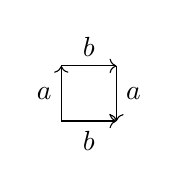
\begin{tikzpicture}[baseline=(current bounding box.center),scale=0.7]
\draw[->] (0,0)--node[left] {$a$}(0,1);
\draw[->] (0,1)--node[above] {$b$}(1,1);
\draw[->] (1,1)--node[right] {$a$}(1,0);
\draw[->] (0,0)--node[below] {$b$}(1,0);
\end{tikzpicture}
\]
and so by dualizing
\[
H^\bullet(G,\mathbb{Z})\cong
\begin{cases}
\mathbb{Z} & \bullet=0,1,\\
\mathbb{Z}/2 & \bullet=2,\\
0 & \text{otherwise}.
\end{cases}
\]
\end{example}

\subsection{Functoriality of group cohomology}
\label{subsec:functoriality}
% Source: handwritten PDF, page 26, originally subsection 1.6.
We conclude this chapter by studying functoriality.
Fix a discrete group $G$ and a nonnegative integer $n$.
We first realize $H^n(G;M)$ as a covariant functor
\[
H^n(G,-):{}_G\mathrm{Mod}\to {}_{\mathbb{Z}}\mathrm{Mod}
\]
and describe its contravariance in the group variable.
% Approved replacement of the imprecise functor formula, already flagged in blue in the source.
For a homomorphism $\varphi:H\to G$, this takes the form of maps
\[
\varphi^*:H^n(G;M)\to H^n(H;\operatorname{res}_{\varphi}M),
\]
where $\operatorname{res}_{\varphi}$ is the restriction functor described below.
We begin with a $G$-module homomorphism $f:M\to N$.

To construct the induced map $f_*:H^n(G;M)\to H^n(G;N)$, we work with cochain complexes.
Choose a projective resolution $P_\bullet\to\mathbb{Z}\to 0$ over $\mathbb{Z}G$ and consider the map of cochain complexes
\[
f_*=f\circ-:\underline{\operatorname{Hom}}_G(P_\bullet,M[0])\to\underline{\operatorname{Hom}}_G(P_\bullet,N[0])
\]
and set
% Approved correction: use cohomology H^n, not H_n.
\[
f_*:=H^n(f_*):H^n(G;M)\to H^n(G;N)
\]
to be our derived map.
These constructions are functorial, giving $H^n(G,-):{}_G\mathrm{Mod}\to {}_{\mathbb{Z}}\mathrm{Mod}$.
% Source: handwritten PDF, page 27.
We next consider functoriality in the group variable.
Consider a group homomorphism $\varphi:H\to G$.
We will construct the induced map $\varphi^*$ on cohomology.
The homomorphism $\varphi$ first gives a functor between module categories
\[
\begin{aligned}
\operatorname{res}_{\varphi}:{}_G\mathrm{Mod}&\to {}_H\mathrm{Mod}\\
(M,a)&\mapsto\operatorname{res}_{\varphi}(M,a)=:\operatorname{res}_{\varphi}M
\end{aligned}
\]
which keeps the underlying abelian group $M$ and gives it the action
\[
\begin{aligned}
\operatorname{res}_{\varphi}(a):H\times\operatorname{res}_{\varphi}(M)&\to\operatorname{res}_{\varphi}(M)\\
(h,m)&\mapsto a(\varphi(h),m).
\end{aligned}
\]
This functor keeps the underlying maps of abelian groups.
Now to get a map
\[
\varphi^*:H^n(G,M)\to H^n(H,\operatorname{res}_{\varphi}M)
\]
on cohomology, we compare a projective resolution $P_\bullet\to\mathbb{Z}\to 0$ over $\mathbb{Z}G$ with a projective resolution $Q_\bullet\to\mathbb{Z}\to 0$ over $\mathbb{Z}H$.
Restriction first gives a map
\[
\underline{\operatorname{Hom}}_G(P_\bullet,M[0])\to\underline{\operatorname{Hom}}_H(\operatorname{res}_{\varphi}P_\bullet,\operatorname{res}_{\varphi}M[0])
\]
by functoriality.
The augmented complex $\operatorname{res}_{\varphi}P_\bullet\to\mathbb{Z}\to 0$ is exact, but its terms need not be projective over $\mathbb{Z}H$.
To solve this problem, we take a projective resolution $Q_\bullet\to\mathbb{Z}\to 0$ of $H$-modules.
Then
% Approved correction: compare both resolutions over Z[0], not res_phi M[0].
\[
% https://q.uiver.app/#q=WzAsNCxbMCwwLCJRX1xcYnVsbGV0Il0sWzEsMCwiXFxtYXRoYmJ7Wn1bMF0iXSxbMCwxLCJcXG9wZXJhdG9ybmFtZXtyZXN9X3tcXHZhcnBoaX1QX1xcYnVsbGV0Il0sWzEsMSwiXFxtYXRoYmJ7Wn1bMF0iXSxbMCwxXSxbMCwyLCIiLDAseyJzdHlsZSI6eyJib2R5Ijp7Im5hbWUiOiJkYXNoZWQifX19XSxbMSwzLCIiLDAseyJsZXZlbCI6Miwic3R5bGUiOnsiaGVhZCI6eyJuYW1lIjoibm9uZSJ9fX1dLFsyLDNdXQ==
\begin{tikzcd}
	{Q_\bullet} & {\mathbb{Z}[0]} \\
	{\operatorname{res}_{\varphi}P_\bullet} & {\mathbb{Z}[0]}
	\arrow[from=1-1, to=1-2]
	\arrow[dashed, from=1-1, to=2-1]
	\arrow[equals, from=1-2, to=2-2]
	\arrow[from=2-1, to=2-2]
\end{tikzcd}
\]
and precomposition gives the map
\[
\begin{aligned}
\underline{\operatorname{Hom}}_G(P_\bullet,M[0])
&\to\underline{\operatorname{Hom}}_H(\operatorname{res}_{\varphi}P_\bullet,\operatorname{res}_{\varphi}M[0])\\
&\to\underline{\operatorname{Hom}}_H(Q_\bullet,\operatorname{res}_{\varphi}M[0]).
\end{aligned}
\]
The comparison theorem for projective resolutions~\cite[Chapter~I]{Bro82} makes the map $Q_\bullet\to\operatorname{res}_{\varphi}P_\bullet$ unique up to chain homotopy, since $Q_\bullet$ is projective in each degree and the target is an exact augmented resolution.
Hence the induced map on cohomology is independent of this lift.
Comparing any two projective resolutions gives chain homotopy equivalences, so the map is also independent of the chosen resolutions.
For $K\xrightarrow{\psi}H\xrightarrow{\varphi}G$, the composite of comparison maps is a comparison map for $\varphi\psi$; uniqueness up to chain homotopy gives $(\varphi\psi)^*=\psi^*\varphi^*$, with the corresponding restrictions of coefficients.
The identity homomorphism induces the identity, and postcomposition with a homomorphism of coefficient modules commutes with these maps.
This proves the asserted functoriality.
% Audit addition approved by the author: independence of choices, identities, composition, and compatibility with coefficients.
% Source: handwritten PDF, page 28, end of the chapter.
\begin{remark}
There is also a topological interpretation.
Let $H$ and $G$ be discrete groups, let $\varphi:H\to G$ be a group homomorphism, and let $M$ be an abelian group with trivial $G$- and $H$-actions.
The classifying space construction $B:\mathrm{Grp}\to\mathrm{CW}_*$ determines a map $B\varphi:BH\to BG$ of pointed CW-complexes.
With these trivial coefficients, we get a map
\[
H^\bullet(B\varphi)=\varphi^*:H^\bullet(BG,M)\to H^\bullet(BH,M)
\]
and so, via the comparison of \autoref{prop:group-twisted-cohomology},
\[
\varphi^*:H^\bullet(G;M)\to H^\bullet(H;M).
\]
% Pink annotation in the source.
Here $\operatorname{res}_{\varphi}M=M$.
\end{remark}
\section{Cohomology of group theoretic constructions}
\label{sec:group-constructions}
% Source: handwritten PDF, page 29, originally Chapter 2.
This chapter develops techniques for computing the cohomology of direct products, amalgamated products, and subgroups.
These computations will be useful in the study of dimensions of groups.
We use functoriality and the interpretation of group cohomology through classifying spaces.

\subsection{Direct products}
\label{subsec:direct-products}
We begin with direct products.
By \autoref{prop:group-twisted-cohomology}, we can start with the corresponding topological result.
For products, this is the following theorem.
For the K\"unneth formula and its cohomological variants, see \cite[Section~3.B]{Hat02} and \cite[Chapter~V]{Bro82}.
\begin{theorem}[K\"unneth]
\label{thm:kunneth-spaces}
Let $X_1,X_2$ be CW-complexes, and assume that the homology groups $H_n(X_1;\mathbb{Z})$ are finitely generated for every $n\geq 0$.
% Approved correction: the finiteness hypothesis concerns homology; the middle term has degree n.
Then, for every $n\geq 0$, there exists a split exact sequence
\[
\begin{aligned}
0\to\bigoplus_{i+j=n}H^i(X_1;\mathbb{Z})\otimes_{\mathbb{Z}}H^j(X_2;\mathbb{Z})
&\to H^n(X_1\times X_2;\mathbb{Z})\\
&\to\bigoplus_{i+j=n+1}\operatorname{Tor}^{\mathbb{Z}}_1\bigl(H^i(X_1;\mathbb{Z}),H^j(X_2;\mathbb{Z})\bigr)\to 0.
\end{aligned}
\]
\end{theorem}
For example, let us apply the coefficient variant of \autoref{thm:kunneth-spaces} explained in \autoref{rem:kunneth-pid}, with coefficients in $\mathbb{Q}$ (but any other field would produce the same result).
Under the corresponding finiteness hypothesis, we claim that there exists an isomorphism
\[
H^n(X_1\times X_2;\mathbb{Q})\cong\bigoplus_{i+j=n}H^i(X_1;\mathbb{Q})\otimes_{\mathbb{Q}}H^j(X_2;\mathbb{Q}).
\]
This follows from the vanishing
\[
\operatorname{Tor}^{\mathbb{Q}}_1\bigl(H^i(X_1;\mathbb{Q}),H^j(X_2;\mathbb{Q})\bigr)=0.
\]
Indeed, every $\mathbb{Q}$-module is free, so these $\operatorname{Tor}$ groups vanish.
Note that the assumptions are clearly satisfied if $X_1$ is constructed by attaching a finite number of cells in each dimension.
% Source: handwritten PDF, page 30.
For discrete groups $G_1,G_2$, we seek a formula for $H^\bullet(G_1\times G_2;\mathbb{Z})$.
The idea is to use the isomorphisms
\[
H^\bullet(G_i;\mathbb{Z})\cong H^\bullet_{\mathrm{tw}}(BG_i;\mathbb{Z})\cong H^\bullet(BG_i;\mathbb{Z})
\]
that relate the group cohomology of $G_i$ with the singular cohomology of the classifying space $BG_i$.
To apply \autoref{thm:kunneth-spaces}, we need an isomorphism
\[
H^\bullet(BG_1\times BG_2;\mathbb{Z})\cong H^\bullet(B(G_1\times G_2);\mathbb{Z}),
\]
and so we need to prove the following lemma.
% Pink annotation: B, being a right adjoint, preserves products.
In products of CW-complexes we use the weak CW topology; see \cite[Section~3.B]{Hat02}.
\begin{lemma}
\label{lem:classifying-space-products}
Let $G_1,G_2$ be discrete groups.
Then $B(G_1\times G_2)\simeq BG_1\times BG_2$.
\end{lemma}
\begin{proof}
We need to show that $BG_1\times BG_2$ is a model for $B(G_1\times G_2)$, that is, it has fundamental group $G_1\times G_2$, and its universal cover is contractible.
However,
\[
\pi_1(BG_1\times BG_2)\cong\pi_1(BG_1)\times\pi_1(BG_2)\cong G_1\times G_2,
\]
since $\pi_1$ preserves products, and since the universal cover of a product is the product of the universal covers, we have
\[
\widetilde{BG_1\times BG_2}\cong\widetilde{BG_1}\times\widetilde{BG_2}\simeq *\times *\simeq *.
\]
\end{proof}
Hence we can apply \autoref{thm:kunneth-spaces} and use the isomorphism in the middle term to get the following theorem.
\begin{theorem}
\label{thm:kunneth-groups}
Let $G_1,G_2$ be discrete groups and suppose that $H_n(G_1;\mathbb{Z})$ is finitely generated for every $n\geq 0$.
Give $\mathbb{Z}$ the trivial action.
Then, for every $n\geq 0$, there exists a split exact sequence
\[
\begin{aligned}
0\to\bigoplus_{i+j=n}H^i(G_1;\mathbb{Z})\otimes_{\mathbb{Z}}H^j(G_2;\mathbb{Z})
&\to H^n(G_1\times G_2;\mathbb{Z})\\
&\to\bigoplus_{i+j=n+1}\operatorname{Tor}^{\mathbb{Z}}_1\bigl(H^i(G_1;\mathbb{Z}),H^j(G_2;\mathbb{Z})\bigr)\to 0.
\end{aligned}
\]
\end{theorem}
\begin{remark}
\label{rem:kunneth-pid}
The K\"unneth formula also holds with coefficients in any principal ideal domain $R$.
Indeed, if $H_n(X_1;R)$ is finitely generated for every $n\geq 0$, then there is a split short exact sequence
\[
\begin{aligned}
0\to\bigoplus_{i+j=n}H^i(X_1;R)\otimes_R H^j(X_2;R)
&\to H^n(X_1\times X_2;R)\\
&\to\bigoplus_{i+j=n+1}\operatorname{Tor}^R_1\bigl(H^i(X_1;R),H^j(X_2;R)\bigr)\to 0.
\end{aligned}
\]
% Source: handwritten PDF, pages 30--31.
% Approved correction: the handwritten denial of this comparison for general R is false for trivial actions.
This statement can also be lifted to group cohomology when $R$ has trivial group action, since by \autoref{prop:group-twisted-cohomology} we have
\[
H^\bullet(G;R)\cong H^\bullet_{\mathrm{tw}}(BG;R)\cong H^\bullet(BG;R).
\]
In particular, we can apply the formula with $\mathbb{Q}$-coefficients.
\end{remark}

\begin{example}
\label{ex:free-abelian-cohomology}
Let $k\geq 1$ and give $\mathbb{Z}$ the trivial $\mathbb{Z}^k$-action.
As an application of \autoref{thm:kunneth-groups}, we compute the cohomology of $\mathbb{Z}^k$ with integer coefficients.
We claim that
\[
H^n(\mathbb{Z}^k;\mathbb{Z})\cong\mathbb{Z}^{\binom{k}{n}},
\]
where $\binom{k}{n}=0$ for $n>k$, and we prove this by induction.
The case $k=1$ is known, so assume the claim for $k-1$ and prove it for $k$.
Since $\mathbb{Z}^k\cong\mathbb{Z}^{k-1}\times\mathbb{Z}$, \autoref{thm:kunneth-groups} says that
% Approved correction: replace the stray X_1,X_2 by the groups in this calculation.
\[
\begin{aligned}
H^n(\mathbb{Z}^{k-1}\times\mathbb{Z};\mathbb{Z})
\cong{}&\bigoplus_{i+j=n}H^i(\mathbb{Z}^{k-1};\mathbb{Z})\otimes_{\mathbb{Z}}H^j(\mathbb{Z};\mathbb{Z})\\
&\oplus\bigoplus_{i+j=n+1}\operatorname{Tor}^{\mathbb{Z}}_1\bigl(H^i(\mathbb{Z}^{k-1};\mathbb{Z}),H^j(\mathbb{Z};\mathbb{Z})\bigr).
\end{aligned}
\]
However, by flatness, the $\operatorname{Tor}$ terms vanish, and the induction hypothesis implies that
\[
\begin{aligned}
H^n(\mathbb{Z}^k;\mathbb{Z})
&\cong\bigl(H^n(\mathbb{Z}^{k-1};\mathbb{Z})\otimes\mathbb{Z}\bigr)\oplus\bigl(H^{n-1}(\mathbb{Z}^{k-1};\mathbb{Z})\otimes\mathbb{Z}\bigr)\\
&\cong\mathbb{Z}^{\binom{k-1}{n}}\oplus\mathbb{Z}^{\binom{k-1}{n-1}}\cong\mathbb{Z}^{\binom{k}{n}}.
\end{aligned}
\]
Here cohomology in negative degrees is zero.
\end{example}
% Source: handwritten PDF, page 32.
\begin{example}
Let $k\geq 1$ and give $\mathbb{Q}$ the trivial $(\mathbb{Z}/2)^k$-action.
Let us compute $H^\bullet((\mathbb{Z}/2)^k;\mathbb{Q})$.
We proceed by induction on $k$.
For $k=1$, we know
\[
H^n(\mathbb{Z}/2;\mathbb{Q})\cong
\begin{cases}
\mathbb{Q} & n=0,\\
0 & n>0.
\end{cases}
\]
Assume the formula for $k$ and consider $k+1$.
% Approved correction: consistent induction indices.
By \autoref{thm:kunneth-groups} and \autoref{rem:kunneth-pid}
\[
H^n((\mathbb{Z}/2)^k\times(\mathbb{Z}/2);\mathbb{Q})\cong\bigoplus_{i+j=n}H^i((\mathbb{Z}/2)^k;\mathbb{Q})\otimes_{\mathbb{Q}}H^j(\mathbb{Z}/2;\mathbb{Q}),
\]
our claim is immediate.
\end{example}
\begin{example}
Let $\ell,k\geq 2$ and give $\mathbb{Z}$ the trivial action.
We now compute $H^\bullet(\mathbb{Z}/\ell\times\mathbb{Z}/k;\mathbb{Z})$.
We apply \autoref{thm:kunneth-groups}: its hypothesis holds since $H_n(\mathbb{Z}/\ell;\mathbb{Z})$ is finitely generated for every $n$.
So we get that
\[
\begin{aligned}
H^n(\mathbb{Z}/\ell\times\mathbb{Z}/k;\mathbb{Z})
\cong{}&\bigoplus_{i+j=n}H^i(\mathbb{Z}/\ell;\mathbb{Z})\otimes H^j(\mathbb{Z}/k;\mathbb{Z})\\
&\oplus\bigoplus_{i+j=n+1}\operatorname{Tor}^{\mathbb{Z}}_1\bigl(H^i(\mathbb{Z}/\ell;\mathbb{Z}),H^j(\mathbb{Z}/k;\mathbb{Z})\bigr).
\end{aligned}
\]
Now recall from \autoref{cor:finite-cyclic-cohomology} that
\[
H^n(\mathbb{Z}/\ell;\mathbb{Z})\cong
\begin{cases}
\mathbb{Z} & n=0,\\
0 & n\text{ odd},\\
\mathbb{Z}/\ell & n\geq 2\text{ even}.
\end{cases}
\]
Substitution gives the desired groups.
% The explicit simplification is not carried out in the handwritten notes.
\end{example}

\subsection{Amalgamated products}
\label{subsec:amalgamated-products}
We next consider amalgamated products.
As before, we begin with the corresponding topological result.
\begin{theorem}[Mayer--Vietoris]
\label{thm:mayer-vietoris-spaces}
Consider a pushout of CW-complexes
\[
% https://q.uiver.app/#q=WzAsNCxbMCwwLCJYXzAiXSxbMSwwLCJYXzEiXSxbMCwxLCJYXzIiXSxbMSwxLCJYIl0sWzAsMSwiZiJdLFswLDIsImoiLDIseyJzdHlsZSI6eyJ0YWlsIjp7Im5hbWUiOiJob29rIiwic2lkZSI6InRvcCJ9fX1dLFsxLDNdLFsyLDNdXQ==
\begin{tikzcd}
	{X_0} & {X_1} \\
	{X_2} & X
	\arrow["f", from=1-1, to=1-2]
	\arrow["j"', hook, from=1-1, to=2-1]
	\arrow[from=1-2, to=2-2]
	\arrow[from=2-1, to=2-2]
\end{tikzcd}
\]
where $j$ is the inclusion of a subcomplex and $f$ is cellular.
Then there exists a long exact sequence
\[
\cdots\to H^n(X;\mathbb{Z})\to H^n(X_1;\mathbb{Z})\oplus H^n(X_2;\mathbb{Z})\to H^n(X_0;\mathbb{Z})\xrightarrow{\partial}H^{n+1}(X;\mathbb{Z})\to\cdots
\]
in cohomology.
% Approved correction: cohomology, not homology.
\end{theorem}
% Source: handwritten PDF, page 33.
We explain the role of the hypotheses in this theorem.
A pushout in $\mathrm{Top}$, or in $\mathrm{CW}$, need not give a Mayer--Vietoris sequence.
A homotopy pushout does give such a sequence.
Let us explain what we mean.
Suppose we are given two maps $X\xleftarrow{f}W\xrightarrow{g}Y$ in $\mathrm{Top}_*$.
We define the \emph{double mapping cylinder} of $f$ and $g$ as the quotient
\[
M(f,g)=\bigl(X\vee(W\wedge I_+)\vee Y\bigr)/{\sim},
\]
where we identify
\[
f(w)\sim(w,0),\qquad g(w)\sim(w,1).
\]
Here $I=[0,1]$ and $I_+$ is obtained by adjoining a disjoint basepoint.
Note that we have two maps $i_X:X\to M(f,g)$ and $i_Y:Y\to M(f,g)$ and a homotopy commutative square
\[
% https://q.uiver.app/#q=WzAsNCxbMCwwLCJXIl0sWzEsMCwiWSJdLFswLDEsIlgiXSxbMSwxLCJNKGYsZykiXSxbMCwxLCJnIl0sWzAsMiwiZiIsMl0sWzEsMywiaV9ZIl0sWzIsMywiaV9YIiwyXV0=
\begin{tikzcd}
	W & Y \\
	X & {M(f,g)}
	\arrow["g", from=1-1, to=1-2]
	\arrow["f"', from=1-1, to=2-1]
	\arrow["{i_Y}", from=1-2, to=2-2]
	\arrow["{i_X}"', from=2-1, to=2-2]
\end{tikzcd}
\]
where the homotopy is $\psi(w,t)=[w,t]$ for all $(w,t)\in W\times I$.
This square is called the \emph{standard homotopy pushout} of $f$ and $g$.
With it we can define what a homotopy pushout is.
Suppose we are given a homotopy commutative square
\[
% https://q.uiver.app/#q=WzAsNCxbMCwwLCJXIl0sWzEsMCwiWSJdLFswLDEsIlgiXSxbMSwxLCJaIl0sWzAsMSwiZyJdLFswLDIsImYiLDJdLFsxLDMsImsiXSxbMiwzLCJoIiwyXV0=
\begin{tikzcd}
	W & Y \\
	X & Z
	\arrow["g", from=1-1, to=1-2]
	\arrow["f"', from=1-1, to=2-1]
	\arrow["k", from=1-2, to=2-2]
	\arrow["h"', from=2-1, to=2-2]
\end{tikzcd}
\]
with a homotopy $F:hf\simeq kg$.
From these data we can construct a comparison map
\[
\theta_F:M(f,g)\to Z,\qquad
\theta_F(x)=h(x),\quad\theta_F([w,t])=F(w,t),\quad\theta_F(y)=k(y),
\]
with which we compare the given square to the standard homotopy pushout.
With this we can give the following definition.
\begin{definition}
\label{def:homotopy-pushout}
A homotopy commutative square of pointed spaces
\[
% https://q.uiver.app/#q=WzAsNCxbMCwwLCJXIl0sWzEsMCwiWSJdLFswLDEsIlgiXSxbMSwxLCJaIl0sWzAsMSwiZyJdLFswLDIsImYiLDJdLFsxLDMsImsiXSxbMiwzLCJoIiwyXV0=
\begin{tikzcd}
	W & Y \\
	X & Z
	\arrow["g", from=1-1, to=1-2]
	\arrow["f"', from=1-1, to=2-1]
	\arrow["k", from=1-2, to=2-2]
	\arrow["h"', from=2-1, to=2-2]
\end{tikzcd}
\]
is said to be a \emph{homotopy pushout} if there exists a homotopy $F:hf\simeq kg$ for which $\theta_F:M(f,g)\to Z$ is a homotopy equivalence.
\end{definition}
% Source: handwritten PDF, page 34.
Hence it is not sufficient for $Z$ to be homotopy equivalent to $M(f,g)$: the homotopy equivalence must be given by $\theta_F$ for some $F:hf\simeq kg$.
\begin{remark}
The homotopy pushout has the universal property ``up to homotopy'': given maps $u:X\to V$ and $v:Y\to V$ with $uf\simeq vg$, there exists $m:Z\to V$ making $mh\simeq u$ and $mk\simeq v$.
% Approved correction: the source interchanges h and k in these composites.
\[
% https://q.uiver.app/#q=WzAsNSxbMCwwLCJXIl0sWzEsMCwiWSJdLFswLDEsIlgiXSxbMSwxLCJaIl0sWzIsMiwiViJdLFswLDEsImciXSxbMCwyLCJmIiwyXSxbMSwzLCJrIl0sWzEsNCwidiIsMCx7ImN1cnZlIjotMX1dLFsyLDMsImgiXSxbMiw0LCJ1IiwyLHsiY3VydmUiOjF9XSxbMyw0LCJtIiwwLHsic3R5bGUiOnsiYm9keSI6eyJuYW1lIjoiZGFzaGVkIn19fV1d
\begin{tikzcd}
	W & Y & \\
	X & Z \\
	&& V
	\arrow["g", from=1-1, to=1-2]
	\arrow["f"', from=1-1, to=2-1]
	\arrow["k", from=1-2, to=2-2]
	\arrow["v", curve={height=-6pt}, from=1-2, to=3-3]
	\arrow["h", from=2-1, to=2-2]
	\arrow["u"', curve={height=6pt}, from=2-1, to=3-3]
	\arrow["m", dashed, from=2-2, to=3-3]
\end{tikzcd}
\]
In the homotopy category this gives a weak pushout: the induced map need not be unique.
\end{remark}
Now what we need is the following proposition.
\begin{proposition}
\label{prop:cofibration-pushout}
Assume that the following commutative square of pointed CW-complexes is a pushout:
\[
% https://q.uiver.app/#q=WzAsNCxbMCwwLCJXIl0sWzEsMCwiWSJdLFswLDEsIlgiXSxbMSwxLCJaLiJdLFswLDEsImciXSxbMCwyLCJmIiwyXSxbMSwzXSxbMiwzXV0=
\begin{tikzcd}
	W & Y \\
	X & {Z.}
	\arrow["g", from=1-1, to=1-2]
	\arrow["f"', from=1-1, to=2-1]
	\arrow[from=1-2, to=2-2]
	\arrow[from=2-1, to=2-2]
\end{tikzcd}
\]
If $f$ or $g$ is a cofibration, then the square is a homotopy pushout.
\end{proposition}
We now return to cohomology.
\begin{example}
Let $X_1,X_2$ be pointed connected CW-complexes, whose basepoints are vertices, and let $X_0=*$.
Our pushout is given by the one-point union $X=X_1\vee X_2$, and so the cohomology of $X$ can be computed by looking at the exact sequence of \autoref{thm:mayer-vietoris-spaces}.
In particular, for $n\geq 1$,
\[
H^n(X_1\vee X_2;\mathbb{Z})\cong H^n(X_1;\mathbb{Z})\oplus H^n(X_2;\mathbb{Z}),
\]
and for $n=0$ we have the exact sequence
\[
0\to H^0(X;\mathbb{Z})\to H^0(X_1;\mathbb{Z})\oplus H^0(X_2;\mathbb{Z})\to H^0(X_0;\mathbb{Z})\to 0,
\]
making
\[
H^0(X_1;\mathbb{Z})\oplus H^0(X_2;\mathbb{Z})\cong\mathbb{Z}\oplus H^0(X;\mathbb{Z}),
\]
since $\mathbb{Z}$ is projective.
\end{example}
% Source: handwritten PDF, page 35.
To obtain a group cohomology analogue, we ask when the classifying space construction takes a pushout of groups to a homotopy pushout of spaces.
That is, if
\[
% https://q.uiver.app/#q=WzAsNCxbMCwwLCJHXzAiXSxbMSwwLCJHXzEiXSxbMCwxLCJHXzIiXSxbMSwxLCJHXFxjb25nIEdfMSpfe0dfMH1HXzIiXSxbMCwxXSxbMCwyXSxbMSwzXSxbMiwzXV0=
\begin{tikzcd}
	{G_0} & {G_1} \\
	{G_2} & {G\cong G_1*_{G_0}G_2}
	\arrow[from=1-1, to=1-2]
	\arrow[from=1-1, to=2-1]
	\arrow[from=1-2, to=2-2]
	\arrow[from=2-1, to=2-2]
\end{tikzcd}
\]
is a pushout of groups, then we want
\[
% https://q.uiver.app/#q=WzAsNCxbMCwwLCJCR18wIl0sWzEsMCwiQkdfMSJdLFswLDEsIkJHXzIiXSxbMSwxLCJCRyJdLFswLDFdLFswLDJdLFsxLDNdLFsyLDNdXQ==
\begin{tikzcd}
	{BG_0} & {BG_1} \\
	{BG_2} & BG
	\arrow[from=1-1, to=1-2]
	\arrow[from=1-1, to=2-1]
	\arrow[from=1-2, to=2-2]
	\arrow[from=2-1, to=2-2]
\end{tikzcd}
\]
to be a homotopy pushout of spaces.
This need not hold in general.
For example, look at
\[
% https://q.uiver.app/#q=WzAsNCxbMCwwLCJcXG1hdGhiYntafSJdLFsxLDAsIjAiXSxbMCwxLCIwIl0sWzEsMSwiMCJdLFswLDFdLFswLDJdLFsxLDNdLFsyLDNdXQ==
\begin{tikzcd}
	{\mathbb{Z}} & 0 \\
	0 & 0
	\arrow[from=1-1, to=1-2]
	\arrow[from=1-1, to=2-1]
	\arrow[from=1-2, to=2-2]
	\arrow[from=2-1, to=2-2]
\end{tikzcd}
\qquad\rightsquigarrow\qquad
% https://q.uiver.app/#q=WzAsNCxbMCwwLCJCXFxtYXRoYmJ7Wn1cXHNpbWVxIFNeMSJdLFsxLDAsIioiXSxbMCwxLCIqIl0sWzEsMSwiKi4iXSxbMCwxXSxbMCwyXSxbMSwzXSxbMiwzXV0=
\begin{tikzcd}
	{B\mathbb{Z}\simeq S^1} & {*} \\
	{*} & {*.}
	\arrow[from=1-1, to=1-2]
	\arrow[from=1-1, to=2-1]
	\arrow[from=1-2, to=2-2]
	\arrow[from=2-1, to=2-2]
\end{tikzcd}
\]
The second square is not a homotopy pushout, since its homotopy pushout is $\Sigma S^1\simeq S^2$.
However, we can prove the following lemma.
\begin{lemma}
\label{lem:classifying-space-amalgam}
Let
\[
% https://q.uiver.app/#q=WzAsNCxbMCwwLCJHXzAiXSxbMSwwLCJHXzEiXSxbMCwxLCJHXzIiXSxbMSwxLCJHIl0sWzAsMSwiIiwwLHsic3R5bGUiOnsidGFpbCI6eyJuYW1lIjoiaG9vayIsInNpZGUiOiJ0b3AifX19XSxbMCwyLCIiLDAseyJzdHlsZSI6eyJ0YWlsIjp7Im5hbWUiOiJob29rIiwic2lkZSI6InRvcCJ9fX1dLFsxLDNdLFsyLDNdXQ==
\begin{tikzcd}
	{G_0} & {G_1} \\
	{G_2} & G
	\arrow[hook, from=1-1, to=1-2]
	\arrow[hook, from=1-1, to=2-1]
	\arrow[from=1-2, to=2-2]
	\arrow[from=2-1, to=2-2]
\end{tikzcd}
\]
be a pushout square of discrete groups where the two maps out of $G_0$ are monomorphisms.
Then there exists a homotopy pushout of CW-complexes
\[
% https://q.uiver.app/#q=WzAsNCxbMCwwLCJCR18wIl0sWzEsMCwiQkdfMSJdLFswLDEsIkJHXzIiXSxbMSwxLCJCRy4iXSxbMCwxXSxbMCwyXSxbMSwzXSxbMiwzXV0=
\begin{tikzcd}
	{BG_0} & {BG_1} \\
	{BG_2} & {BG.}
	\arrow[from=1-1, to=1-2]
	\arrow[from=1-1, to=2-1]
	\arrow[from=1-2, to=2-2]
	\arrow[from=2-1, to=2-2]
\end{tikzcd}
\]
\end{lemma}
\begin{proof}
Let $X_i=BG_i$ and let $X$ be the homotopy pushout of $BG_1\leftarrow BG_0\to BG_2$.
We want to show that $X$ is homotopy equivalent to $BG$, for $G=G_1*_{G_0}G_2$.
We verify that $X$ is a model for $BG$.
The Seifert--van Kampen theorem gives $\pi_1(X)\cong G$, so it remains to show that $\widetilde X$ is contractible.
% Approved correction: pi_1(X)=G, not pi_1(G).
To show that $\widetilde{X}$ is contractible, we use \autoref{cor:acyclic-simply-connected}: a CW-complex $Y$ is contractible if and only if it is simply connected and acyclic.
The universal cover $\widetilde X$ is simply connected, so it suffices to prove acyclicity.
% Source: handwritten PDF, page 36.
% Approved repair: use pullbacks of the universal cover, not the inconsistent pushout diagram in the source.
Denote by $p:\widetilde{X}\to X$ the covering map, and use mapping cylinders to regard the $X_i$ as subcomplexes with $X=X_1\cup_{X_0}X_2$.
Then
\[
\widetilde{X}=p^{-1}(X_1)\cup_{p^{-1}(X_0)}p^{-1}(X_2).
\]
Note that the spaces $p^{-1}(X_i)$ need not be connected.
Let $A^i_\alpha\subseteq p^{-1}(X_i)$ be a path component, and choose a basepoint in it.
The pullback square
\[
% https://q.uiver.app/#q=WzAsNCxbMCwwLCJwXnstMX0oWF9pKSJdLFsxLDAsIlxcd2lkZXRpbGRle1h9Il0sWzAsMSwiWF9pIl0sWzEsMSwiWCJdLFswLDFdLFswLDIsInAiLDJdLFsxLDMsInAiXSxbMiwzXV0=
\begin{tikzcd}
	{p^{-1}(X_i)} & {\widetilde{X}} \\
	{X_i} & X
	\arrow[from=1-1, to=1-2]
	\arrow["p"', from=1-1, to=2-1]
	\arrow["p", from=1-2, to=2-2]
	\arrow[from=2-1, to=2-2]
\end{tikzcd}
\]
shows that $A^i_\alpha\to X_i$ is a connected covering.
The induced map $\pi_1(A^i_\alpha)\to\pi_1(X_i)=G_i$ is injective, and its composite with the injection $G_i\hookrightarrow G$ is zero, since it factors through $\pi_1(\widetilde{X})=0$.
Hence $\pi_1(A^i_\alpha)=0$, making $A^i_\alpha$ the universal cover of $X_i$.
Thus $A^i_\alpha$ is contractible.
Mayer--Vietoris now gives $H_n(\widetilde{X};\mathbb{Z})=0$ for $n\geq 2$.
Also $H_1(\widetilde{X};\mathbb{Z})=0$ since $\widetilde{X}$ is simply connected.
Therefore $\widetilde{X}$ is acyclic, as required.
\end{proof}
Hence \autoref{lem:classifying-space-amalgam}, combined with \autoref{thm:mayer-vietoris-spaces}, allows us to prove the following theorem.
\begin{theorem}[Mayer--Vietoris]
\label{thm:mayer-vietoris-groups}
Let $G_0\hookrightarrow G_1$ and $G_0\hookrightarrow G_2$ be monomorphisms of discrete groups, and put $G=G_1*_{G_0}G_2$.
With trivial integer coefficients, there exists a long exact sequence
\[
\cdots\to H^n(G;\mathbb{Z})\to H^n(G_1;\mathbb{Z})\oplus H^n(G_2;\mathbb{Z})\to H^n(G_0;\mathbb{Z})\xrightarrow{\partial}H^{n+1}(G;\mathbb{Z})\to\cdots.
\]
\end{theorem}
% Source: handwritten PDF, page 37.
% Approved correction: the source incorrectly rules out general coefficients altogether.
Let us point out that the argument just given uses trivial coefficients, through the comparison $H^\bullet(G;\mathbb{Z})\cong H^\bullet(BG;\mathbb{Z})$.
The more general version uses local coefficients.
Anyway, injectivity is necessary in \autoref{thm:mayer-vietoris-groups}.
Indeed, the square
\[
% https://q.uiver.app/#q=WzAsNCxbMCwwLCIyXFxtYXRoYmJ7Wn0iXSxbMSwwLCJcXG1hdGhiYntafSJdLFswLDEsIjAiXSxbMSwxLCJcXG1hdGhiYntafS8yXFxtYXRoYmJ7Wn0iXSxbMCwxLCIiLDAseyJzdHlsZSI6eyJ0YWlsIjp7Im5hbWUiOiJob29rIiwic2lkZSI6InRvcCJ9fX1dLFswLDJdLFsxLDNdLFsyLDNdXQ==
\begin{tikzcd}
	{2\mathbb{Z}} & {\mathbb{Z}} \\
	0 & {\mathbb{Z}/2\mathbb{Z}}
	\arrow[hook, from=1-1, to=1-2]
	\arrow[from=1-1, to=2-1]
	\arrow[from=1-2, to=2-2]
	\arrow[from=2-1, to=2-2]
\end{tikzcd}
\]
is a pushout of groups, but $H^\bullet(\mathbb{Z}/2;\mathbb{Z})$ is nontrivial in arbitrarily high degrees.
As an application, let us compute the cohomology of the free product.
For discrete groups $G_1,G_2$, the free product is a pushout along inclusions of the trivial group, giving
\[
BG_1\vee BG_2\simeq B(G_1*G_2).
\]
The Mayer--Vietoris sequence therefore gives
\[
0\to H^n(G_1*G_2;\mathbb{Z})\to H^n(G_1;\mathbb{Z})\oplus H^n(G_2;\mathbb{Z})\to 0
\]
for $n\geq 1$, and
\[
0\to H^0(G_1*G_2;\mathbb{Z})\to H^0(G_1;\mathbb{Z})\oplus H^0(G_2;\mathbb{Z})\to\mathbb{Z}\to 0,
\]
making
% Approved correction: free product, not wedge of groups; write degree zero explicitly.
\[
H^n(G_1*G_2;\mathbb{Z})\cong
\begin{cases}
\mathbb{Z}&n=0,\\
H^n(G_1;\mathbb{Z})\oplus H^n(G_2;\mathbb{Z})&n\geq 1.
\end{cases}
\]
\begin{example}
\label{ex:infinite-dihedral-cohomology}
We can compute the cohomology of the infinite dihedral group
\[
D_\infty=\langle t,s\mid s^2=1,\ sts=t^{-1}\rangle\cong\mathbb{Z}\rtimes\mathbb{Z}/2\mathbb{Z},
\]
where the action is by inversion and the coefficient action on $\mathbb{Z}$ is trivial.
This group is the symmetry group of the degenerate ``$n$-gon'', for $n\to+\infty$.
How do we compute its cohomology?
We note that
\[
D_\infty\cong\mathbb{Z}/2\mathbb{Z}*\mathbb{Z}/2\mathbb{Z}=\langle s_1,s_2\mid s_1^2=s_2^2=1\rangle,
\qquad t\mapsto s_1s_2,\quad s\mapsto s_1,
\]
and so the pushout
% Source: handwritten PDF, page 38.
\[
% https://q.uiver.app/#q=WzAsNCxbMCwwLCIwIl0sWzEsMCwiXFxtYXRoYmJ7Wn0vMlxcbWF0aGJie1p9Il0sWzAsMSwiXFxtYXRoYmJ7Wn0vMlxcbWF0aGJie1p9Il0sWzEsMSwiRF9cXGluZnR5Il0sWzAsMV0sWzAsMl0sWzEsM10sWzIsM11d
\begin{tikzcd}
	0 & {\mathbb{Z}/2\mathbb{Z}} \\
	{\mathbb{Z}/2\mathbb{Z}} & {D_\infty}
	\arrow[from=1-1, to=1-2]
	\arrow[from=1-1, to=2-1]
	\arrow[from=1-2, to=2-2]
	\arrow[from=2-1, to=2-2]
\end{tikzcd}
\]
gives us the long exact sequence of \autoref{thm:mayer-vietoris-groups}.
Therefore
\[
\begin{aligned}
\widetilde{H}^n(D_\infty;\mathbb{Z})
&\cong\widetilde{H}^n(\mathbb{Z}/2\mathbb{Z};\mathbb{Z})\oplus\widetilde{H}^n(\mathbb{Z}/2\mathbb{Z};\mathbb{Z})\\
&\cong
\begin{cases}
0&n=0\text{ or }n\text{ odd},\\
(\mathbb{Z}/2\mathbb{Z})^2&n\geq 2\text{ even}.
\end{cases}
\end{aligned}
\]
Moreover, with trivial rational coefficients,
\[
\widetilde{H}^\bullet(D_\infty;\mathbb{Q})\cong\widetilde{H}^\bullet(\mathbb{Z}/2\mathbb{Z};\mathbb{Q})\oplus\widetilde{H}^\bullet(\mathbb{Z}/2\mathbb{Z};\mathbb{Q})=0.
\]
% Editorial note (2026-10-29): the author does not recall the intended comparison, so the sentence is retained only in the source without supplying an interpretation.
% Original sentence: It is surprising since $D_\infty$ is not far from being the rationals.
\end{example}
\subsection{Right-angled Coxeter and Artin groups}
\label{subsec:coxeter-artin}
% Source: handwritten PDF, page 38, originally subsection 2.3.
Before turning to subgroups, we apply these methods to right-angled Coxeter and Artin groups.
These groups lead to proposed counterexamples to \autoref{conj:eilenberg-ganea}.
Their definitions use finite simplicial graphs.
A \emph{finite simplicial graph}, or \emph{simple graph}, is a finite graph $\Gamma=(V,E)$ that has no loops and no multiple edges.
% Approved correction: include the exclusion of multiple edges, already indicated by the source drawings.
For example,
\[
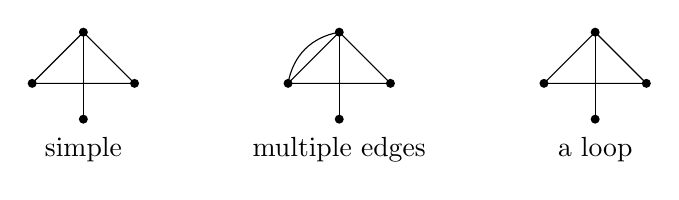
\begin{tikzpicture}[scale=.65]
\draw (0,1)--(-1,0)--(1,0)--cycle;
\draw (0,1)--(0,-.7);
\foreach \x/\y in {0/1,-1/0,1/0,0/-.7}{\fill (\x,\y) circle (2.5pt);}
\node at (0,-1.3) {simple};
\begin{scope}[xshift=5cm]
\draw (0,1)--(-1,0)--(1,0)--cycle;
\draw (0,1) to[bend right=35] (-1,0);
\draw (0,1)--(0,-.7);
\foreach \x/\y in {0/1,-1/0,1/0,0/-.7}{\fill (\x,\y) circle (2.5pt);}
\node at (0,-1.3) {multiple edges};
\end{scope}
\begin{scope}[xshift=10cm]
\draw (0,1)--(-1,0)--(1,0)--cycle;
\draw (0,1)--(0,-.7);
\draw (1,0) to[out=20,in=110,looseness=6] (1,0);
\foreach \x/\y in {0/1,-1/0,1/0,0/-.7}{\fill (\x,\y) circle (2.5pt);}
\node at (0,-1.3) {a loop};
\end{scope}
\end{tikzpicture}
\]
To a finite simplicial graph $\Gamma=(V,E)$ we can associate a group.
\begin{definition}
\label{def:right-angled-coxeter}
Let $\Gamma=(V,E)$ be a finite simplicial graph.
The \emph{right-angled Coxeter group} associated to $\Gamma$ is the group $W_\Gamma$ presented as
\[
W_\Gamma=\langle s\in V\mid s^2=1,\ [s_i,s_j]=1\text{ if }\{s_i,s_j\}\in E\rangle.
\]
\end{definition}
% Source: handwritten PDF, page 39.
We consider some examples.
\begin{example}
\label{ex:coxeter-basic}
Let $\Gamma$ be a finite simplicial graph.
\begin{enumerate}
\item If $\Gamma$ has one vertex, then $W_\Gamma=\langle s\mid s^2=1\rangle\cong\mathbb{Z}/2$ is finite cyclic of order two.
\item If $\Gamma$ consists of two isolated vertices, then $W_\Gamma=\langle s,t\mid s^2=t^2=1\rangle\cong\mathbb{Z}/2*\mathbb{Z}/2$ is a free product.
\item If $\Gamma$ consists of one edge and its two endpoints, then $W_\Gamma\cong\mathbb{Z}/2\times\mathbb{Z}/2$, as the presentation shows.
\item For graphs with at least three vertices, further cases arise.
First of all, the discrete graph on three vertices and the triangle produce $\mathop{*}_{i=1}^3\mathbb{Z}/2$ and $\prod_{i=1}^3\mathbb{Z}/2$, respectively.
The graph with three vertices and one edge produces $(\mathbb{Z}/2\times\mathbb{Z}/2)*\mathbb{Z}/2$, and the path with three vertices produces
\[
\begin{aligned}
W_\Gamma&=\langle s,t,v\mid s^2=t^2=v^2=1,\ [s,t]=[s,v]=1\rangle\\
&\cong(\mathbb{Z}/2)^2*_{\mathbb{Z}/2}(\mathbb{Z}/2)^2\cong\mathbb{Z}/2\times D_\infty.
\end{aligned}
\]
\end{enumerate}
\end{example}
These examples suggest the following general formulas:
\begin{enumerate}
\item if the graph $\Gamma$ is discrete, that is, $E=\varnothing$, then $W_\Gamma\cong\mathop{*}_{v\in V}\mathbb{Z}/2$;
\item if the graph $\Gamma$ is complete, that is, every two distinct vertices are connected by an edge, then $W_\Gamma\cong\prod_{v\in V}\mathbb{Z}/2$.
\end{enumerate}
We also have the following lemma.
\begin{lemma}
\label{lem:coxeter-full-subgraph}
Let $\Gamma$ be a finite simplicial graph and let $\Lambda\subseteq\Gamma$ be a full subgraph, that is, every edge of $\Gamma$ between vertices of $\Lambda$ also belongs to $\Lambda$.
Then $W_\Lambda\to W_\Gamma$ is a split injection.
\end{lemma}
\begin{proof}
Indeed, the map $W_\Lambda\to W_\Gamma$ admits a left inverse $W_\Gamma\to W_\Lambda$ defined by fixing the generators in $\Lambda$ and sending every generator outside $\Lambda$ to $1$.
% Approved correction: kill generators outside Lambda, not all elements outside W_Lambda.
\end{proof}
The amalgamated-product example generalizes as follows.
% Source: handwritten PDF, page 40.
\begin{lemma}
\label{lem:coxeter-amalgam}
Let $\Gamma$ be a finite simplicial graph and suppose $\Gamma=\Gamma_1\cup_{\Gamma_0}\Gamma_2$, where $\Gamma_1,\Gamma_2$ are full subgraphs and $\Gamma_0=\Gamma_1\cap\Gamma_2$.
Then
\[
W_\Gamma\cong W_{\Gamma_1}*_{W_{\Gamma_0}}W_{\Gamma_2}.
\]
\end{lemma}
The term ``right-angled'' has a geometric interpretation.
We can view the generators as reflections across hyperplanes, with commutation relations corresponding to perpendicular hyperplanes.
For example, consider the square graph and its associated group $W_\Gamma=D_\infty\times D_\infty$.
The vertices of $\Gamma$ are now reflections that act on $\mathbb{R}^2$:
\[
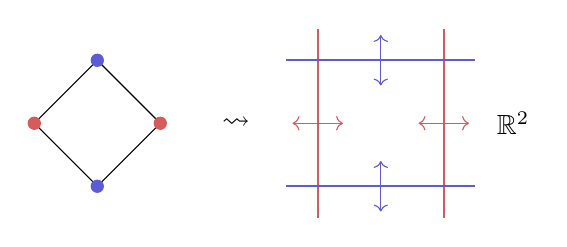
\begin{tikzpicture}[scale=.8]
\draw (0,1)--(1,0)--(0,-1)--(-1,0)--cycle;
\fill[AcyclicBlue] (0,1) circle (3pt) (0,-1) circle (3pt);
\fill[AcyclicPink] (1,0) circle (3pt) (-1,0) circle (3pt);
\node at (2.2,0) {$\rightsquigarrow$};
\draw[AcyclicPink,thick] (3.5,-1.5)--(3.5,1.5) (5.5,-1.5)--(5.5,1.5);
\draw[AcyclicBlue,thick] (3,-1)--(6,-1) (3,1)--(6,1);
\node at (6.6,0) {$\mathbb{R}^2$};
\draw[<->,AcyclicPink] (3.1,0)--(3.9,0);
\draw[<->,AcyclicPink] (5.1,0)--(5.9,0);
\draw[<->,AcyclicBlue] (4.5,.6)--(4.5,1.4);
\draw[<->,AcyclicBlue] (4.5,-.6)--(4.5,-1.4);
\end{tikzpicture}
\]
The reflections corresponding to adjacent vertices commute.
We next prove a result about the commutator subgroup.
\begin{lemma}
\label{lem:coxeter-commutator}
For a finite simplicial graph $\Gamma$, the group $[W_\Gamma,W_\Gamma]$ is torsion-free and of finite index in $W_\Gamma$.
\end{lemma}
\begin{proof}
We first show that every finite subgroup $F\subseteq W_\Gamma$ is conjugate into $W_\Lambda$ for some complete subgraph $\Lambda\subseteq\Gamma$.
% Approved correction: conjugate into a special subgroup, not equal to it.
We use the following fact: a finite subgroup of $G_1*_{G_0}G_2$, with injective amalgamating maps, is conjugate into $G_1$ or $G_2$.
We proceed by induction on the number of vertices of $\Gamma$.
If $\Gamma$ is complete, then $W_\Gamma\cong\prod_{v\in V}\mathbb{Z}/2$ and the claim is trivial.
If $\Gamma$ is not complete, then $\Gamma=\Gamma_1\cup_{\Gamma_0}\Gamma_2$, where the $\Gamma_i$ are full subgraphs with fewer vertices than $\Gamma$.
Now by the general fact there exists $g\in W_\Gamma$ such that $gFg^{-1}\subseteq W_{\Gamma_1}$, for example.
By induction, there exists $h\in W_{\Gamma_1}$ such that $(hg)F(hg)^{-1}\subseteq W_{\Lambda_1}$, with $\Lambda_1\subseteq\Gamma_1\subseteq\Gamma$ complete.
% Source: handwritten PDF, page 41.
Now consider the exact sequence
\[
1\to[W_\Gamma,W_\Gamma]\to W_\Gamma\xrightarrow{\pi}\prod_{v\in V}\mathbb{Z}/2\to 1
\]
given by the abelianization map $\pi$.
The quotient is finite, so $[W_\Gamma,W_\Gamma]$ has finite index.
Let $F\subseteq W_\Gamma$ be a nontrivial finite subgroup.
We show that $\pi(F)\neq 1$, so that $F\nsubseteq\ker(\pi)=[W_\Gamma,W_\Gamma]$, which then has no torsion.
By the preceding argument, there exists $g\in W_\Gamma$ with $gFg^{-1}\subseteq W_\Lambda$ for some complete $\Lambda\subseteq\Gamma$.
This happens if and only if $F\subseteq g^{-1}W_\Lambda g$, but the map
\[
\pi|_{g^{-1}W_\Lambda g}:g^{-1}W_\Lambda g\to\prod_{v\in V}\mathbb{Z}/2
\]
is injective since $\Lambda$ is complete.
Hence $\pi(F)\neq 1$.
\end{proof}
We can now compute rational cohomology using the methods developed above.
Indeed, we can prove the following theorem.
\begin{theorem}
\label{thm:coxeter-rational-cohomology}
Let $\Gamma$ be a finite simplicial graph, and give $\mathbb{Q}$ the trivial $W_\Gamma$-action.
Then
\[
H^n(W_\Gamma;\mathbb{Q})\cong
\begin{cases}
\mathbb{Q}&n=0,\\
0&n\geq 1.
\end{cases}
\]
\end{theorem}
\begin{proof}
We proceed by induction on the number of vertices of $\Gamma$.
For the empty graph $W_\Gamma=1$, and for $|V|=1$ we have $W_\Gamma\cong\mathbb{Z}/2$, so the statement is clearly true.
% Approved addition: the empty graph is needed when a vertex is isolated.
So let us assume the statement for every graph $\Lambda$ with $|V^\Lambda|<|V^\Gamma|$, and let us prove it for $\Gamma$.
We distinguish the complete and noncomplete graphs.
By \autoref{def:right-angled-coxeter}, if $\Gamma$ is complete, then $W_\Gamma\cong\prod_{v\in V}\mathbb{Z}/2$, and so \autoref{thm:kunneth-groups} and \autoref{rem:kunneth-pid} allow us to conclude.
Therefore, we can assume that $\Gamma$ is not complete.
% Source: handwritten PDF, page 42.
Then we can find $v\in V$ which is not connected to all other vertices, that is, there exists $w\neq v$ with $\{v,w\}\notin E$.
The idea now is to decompose $\Gamma=\Gamma_1\cup_{\Gamma_0}\Gamma_2$ into full subgraphs:
\begin{itemize}
\item $\Gamma_1$ is spanned by $v$ and all vertices connected to it;
\item $\Gamma_0$ is spanned by all vertices connected to $v$, but not $v$;
\item $\Gamma_2$ is spanned by $V\setminus\{v\}$.
\end{itemize}
\[
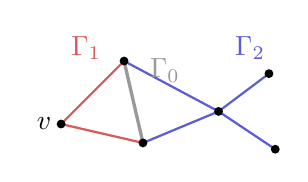
\begin{tikzpicture}[scale=.8]
\draw[AcyclicPink,thick] (0,0)--(1,1)--(1.3,-.3)--cycle;
\draw[AcyclicGrey,very thick] (1,1)--(1.3,-.3);
\draw[AcyclicBlue,thick] (1,1)--(2.5,.2)--(1.3,-.3) (2.5,.2)--(3.3,.8) (2.5,.2)--(3.4,-.4);
\foreach \x/\y in {0/0,1/1,1.3/-.3,2.5/.2,3.3/.8,3.4/-.4}{\fill (\x,\y) circle (2pt);}
\node[left] at (0,0) {$v$};
\node[AcyclicPink] at (.4,1.2) {$\Gamma_1$};
\node[AcyclicGrey] at (1.65,.85) {$\Gamma_0$};
\node[AcyclicBlue] at (3,1.2) {$\Gamma_2$};
\end{tikzpicture}
\]
By \autoref{lem:coxeter-amalgam},
\[
W_\Gamma\cong W_{\Gamma_1}*_{W_{\Gamma_0}}W_{\Gamma_2},
\]
and $W_{\Gamma_0}\to W_{\Gamma_1}$ and $W_{\Gamma_0}\to W_{\Gamma_2}$ are monomorphisms.
So by Mayer--Vietoris we get a long exact sequence
\[
\cdots\to H^{n-1}(W_{\Gamma_0};\mathbb{Q})\to H^n(W_\Gamma;\mathbb{Q})\to H^n(W_{\Gamma_1};\mathbb{Q})\oplus H^n(W_{\Gamma_2};\mathbb{Q})\to\cdots.
\]
But now we can use induction, since $\Gamma_0,\Gamma_1,\Gamma_2$ all have fewer vertices than $\Gamma$.
Indeed, $v\notin\Gamma_0,\Gamma_2$, while $w\notin\Gamma_1$.
We conclude that $H^n(W_\Gamma;\mathbb{Q})=0$ for $n\geq 2$.
% Approved repair: the argument in degree one also needs the map on degree-zero cohomology.
For $n=1$, the map $H^0(W_{\Gamma_1};\mathbb{Q})\oplus H^0(W_{\Gamma_2};\mathbb{Q})\to H^0(W_{\Gamma_0};\mathbb{Q})$ is the surjection $(a,b)\mapsto a-b$, so exactness also gives $H^1(W_\Gamma;\mathbb{Q})=0$.
\end{proof}
Together with right-angled Coxeter groups, there are also right-angled Artin groups.
\begin{definition}
\label{def:right-angled-artin}
Let $\Gamma=(V,E)$ be a finite simplicial graph.
The \emph{right-angled Artin group} associated to $\Gamma$ is
\[
A_\Gamma=\langle s\in V\mid [s_i,s_j]=1\text{ if }\{s_i,s_j\}\in E\rangle.
\]
\end{definition}
As before, let us have a look at the examples.
\begin{example}
Let $\Gamma$ be a finite simplicial graph.
\begin{enumerate}
\item If $\Gamma$ has one vertex, then $A_\Gamma\cong\mathbb{Z}$.
Similarly, if $E=\varnothing$, then $A_\Gamma\cong\mathop{*}_{v\in V}\mathbb{Z}$.
% Approved correction: free product, not direct product, for a discrete graph.
\item If $\Gamma$ consists of one edge and its endpoints, then $A_\Gamma\cong\mathbb{Z}\times\mathbb{Z}$.
Similarly, if $\Gamma$ is complete, then $A_\Gamma\cong\prod_{v\in V}\mathbb{Z}$.
\end{enumerate}
\end{example}
These examples parallel the Coxeter-group examples, with $\mathbb{Z}$ replacing $\mathbb{Z}/2$.
% Source: handwritten PDF, page 43.
In this picture we have replaced reflections, given by $\mathbb{Z}/2$, by translations, given by $\mathbb{Z}$.
As before, we can show that if $\Gamma=\Gamma_1\cup_{\Gamma_0}\Gamma_2$ is a union of full subgraphs with intersection $\Gamma_0$, then
\[
A_\Gamma\cong A_{\Gamma_1}*_{A_{\Gamma_0}}A_{\Gamma_2}.
\]

We now compute the cohomology of these groups.
\begin{theorem}
\label{thm:artin-cohomology}
Let $\Gamma$ be a finite simplicial graph and let $n\geq 0$.
Give $\mathbb{Z}$ the trivial $A_\Gamma$-action.
Then
\[
H^n(A_\Gamma;\mathbb{Z})\cong\bigoplus_{\substack{\Lambda\subseteq\Gamma\text{ complete}\\|V^\Lambda|=n}}\mathbb{Z},
\]
where the empty subgraph is included when $n=0$.
\end{theorem}
\begin{proof}
We again proceed by induction on the number of vertices of $\Gamma$.
For the empty graph the statement is immediate.
If $|V|=1$, then
\[
H^n(A_\Gamma;\mathbb{Z})\cong H^n(\mathbb{Z};\mathbb{Z})\cong
\begin{cases}
\mathbb{Z}&n=0,1,\\
0&n\geq 2,
\end{cases}
\]
as computed in \autoref{subsec:cyclic-groups}.
So let us assume the claim for every graph $\Lambda$ with $|V^\Lambda|<|V^\Gamma|$, and let us prove it for $\Gamma$.
We distinguish the complete and noncomplete graphs.
If $\Gamma$ is complete, then $A_\Gamma\cong\prod_{v\in V}\mathbb{Z}$, and we can use \autoref{thm:kunneth-groups} once more to conclude.
So let us assume that $\Gamma$ is not complete, so that we can find a vertex $v\in V$ which is not connected to all other vertices.
In particular, we can decompose $\Gamma=\Gamma_1\cup_{\Gamma_0}\Gamma_2$ using the full subgraphs
\begin{itemize}
\item $\Gamma_1$ is spanned by $v$ and all vertices connected to it;
\item $\Gamma_0$ is spanned by all vertices connected to $v$, but not $v$;
\item $\Gamma_2$ is spanned by $V\setminus\{v\}$.
\end{itemize}
The induction hypothesis applies.
Now, as before,
\[
A_\Gamma\cong A_{\Gamma_1}*_{A_{\Gamma_0}}A_{\Gamma_2},
\]
where all the maps out of $A_{\Gamma_0}$ are monomorphisms.
By \autoref{thm:mayer-vietoris-groups} we can use the long exact sequence
% Source: handwritten PDF, page 44.
\[
\cdots\to H^{n-1}(A_{\Gamma_0};\mathbb{Z})\to H^n(A_\Gamma;\mathbb{Z})\to H^n(A_{\Gamma_1};\mathbb{Z})\oplus H^n(A_{\Gamma_2};\mathbb{Z})\to H^n(A_{\Gamma_0};\mathbb{Z})\to\cdots.
\]
Now if we define
\[
r_n(\Gamma)=\#\{\text{complete subgraphs of }\Gamma\text{ with }n\text{ vertices}\},
\]
we can count these subgraphs.
Since $\Gamma_0\subseteq\Gamma_1$ is full, $A_{\Gamma_0}\to A_{\Gamma_1}$ is a split injection, by the same retraction as in \autoref{lem:coxeter-full-subgraph}.
By applying the cohomology functor, we see that $H^n(A_{\Gamma_1};\mathbb{Z})\to H^n(A_{\Gamma_0};\mathbb{Z})$ is an epimorphism in every degree, giving us the short exact sequence
\[
0\to H^n(A_\Gamma;\mathbb{Z})\to H^n(A_{\Gamma_1};\mathbb{Z})\oplus H^n(A_{\Gamma_2};\mathbb{Z})\to H^n(A_{\Gamma_0};\mathbb{Z})\to 0.
\]
In particular, we see that $H^n(A_\Gamma;\mathbb{Z})$ is free, say $\mathbb{Z}^x$.
The sequence allows us to conclude that
\[
x=r_n(\Gamma_1)+r_n(\Gamma_2)-r_n(\Gamma_0)=r_n(\Gamma).
\]
\end{proof}
\subsection{Subgroups and Shapiro's lemma}
\label{subsec:shapiro}
% Source: handwritten PDF, page 44, originally subsection 2.4.
We now study the relation between the cohomology of a group and that of its subgroups.
Let $H\leq G$ be a subgroup of a discrete group, and let $i:H\hookrightarrow G$ be the inclusion homomorphism.
We first examine the induced functors between their module categories.
We begin by studying the restriction functor
\[
\operatorname{res}^G_H=\operatorname{res}_i:{}_G\mathrm{Mod}\to{}_H\mathrm{Mod}
\]
that sends $(M,a:G\times M\to M)$ to $(M,a\circ(i\times 1_M):H\times M\to M)$, simply restricting the action of $G$ to $H$.
We begin with some examples.
\begin{example}
Let $H\leq G$ be a subgroup of a discrete group, and let $M,N$ be left $\mathbb{Z}G$-modules.
\begin{enumerate}
\item We claim that $\operatorname{res}^G_H(\mathbb{Z})=\mathbb{Z}$ when $\mathbb{Z}$ has trivial action.
Restricting a trivial action gives a trivial action.
% Source: handwritten PDF, page 45.
\item We claim that
\[
\operatorname{res}^G_H(\mathbb{Z}G)\cong\bigoplus_{H\backslash G}\mathbb{Z}H.
\]
Indeed, by restricting the action of $G$ on $\mathbb{Z}G$ we get a free $H$-module with a basis given by representatives of $H\backslash G$.
% Approved correction: right cosets H\G index the left ZH-module decomposition.
\item We claim that $\operatorname{res}^G_H(M\oplus N)\cong\operatorname{res}^G_H(M)\oplus\operatorname{res}^G_H(N)$.
\end{enumerate}
\end{example}
These computations give the following homological properties.
\begin{lemma}
\label{lem:restriction-projectives}
Let $H\leq G$ be a subgroup of a discrete group.
The functor $\operatorname{res}^G_H:{}_G\mathrm{Mod}\to{}_H\mathrm{Mod}$ is exact and preserves projectives.
\end{lemma}
\begin{proof}
The functor $\operatorname{res}^G_H$ is exact, since exactness can be checked on the underlying abelian groups.
It preserves projectives, since projective modules are direct summands of free modules and restriction preserves both freeness and direct summands.
\end{proof}
Now, together with the restriction functor, we should consider the \emph{induction functor}
\[
\begin{aligned}
\operatorname{ind}^G_H:{}_H\mathrm{Mod}&\to{}_G\mathrm{Mod}\\
N&\mapsto\operatorname{ind}^G_H(N)=\mathbb{Z}G\otimes_{\mathbb{Z}H}N.
\end{aligned}
\]
To be more precise, the action of $G$ is given by
\[
g\cdot(g'\otimes n)=gg'\otimes n,
\]
that is, on the left, whereas the tensor product uses the right $\mathbb{Z}H$-action on $\mathbb{Z}G$.
Induction is related to restriction by the following adjunction.
\begin{lemma}
\label{lem:induction-adjunction}
Let $H\leq G$ be a subgroup of a discrete group.
There exists an adjunction
\[
\operatorname{ind}^G_H:{}_H\mathrm{Mod}\rightleftarrows{}_G\mathrm{Mod}:\operatorname{res}^G_H.
\]
\end{lemma}
\begin{proof}
We construct the bijection
\[
\operatorname{Hom}_G(\operatorname{ind}^G_H(N),M)\cong\operatorname{Hom}_H(N,\operatorname{res}^G_H(M))
\]
for every left $\mathbb{Z}H$-module $N$ and left $\mathbb{Z}G$-module $M$.
The two directions are
\[
f\mapsto F_f,\quad F_f(g\otimes n)=g\cdot f(n),
\qquad T\mapsto f_T,\quad f_T(n)=T(e_G\otimes n).
\]
If we start with $f:N\to\operatorname{res}^G_H(M)$ and then construct $F_f$ and $f_{F_f}$, we can compute
\[
f_{F_f}(n)=F_f(e_G\otimes n)=e_G\cdot f(n)=f(n)
\]
for every $n\in N$, proving that one composite is the identity.
% Source: handwritten PDF, page 46.
For the other, start with $T$ and construct $F_{f_T}$.
Then for every $n\in N$ and $g\in G$ we have
\[
F_{f_T}(g\otimes n)=g\cdot f_T(n)=g\cdot T(e_G\otimes n)=T(g\otimes n).
\]
\end{proof}
We consider two examples.
\begin{example}
Let $H\leq G$ be a subgroup of a discrete group.
\begin{enumerate}
\item By a straightforward computation, with trivial $H$-action on $\mathbb{Z}$,
\[
\operatorname{ind}^G_H(\mathbb{Z})=\mathbb{Z}G\otimes_{\mathbb{Z}H}\mathbb{Z}\cong\mathbb{Z}[G/H],
\]
since $\mathbb{Z}G\cong\bigoplus_{G/H}\mathbb{Z}H$ as a right $\mathbb{Z}H$-module.
% Approved clarification: this decomposition uses the right module structure.
\item We have
\[
\operatorname{ind}^G_H(\mathbb{Z}H)=\mathbb{Z}G\otimes_{\mathbb{Z}H}\mathbb{Z}H\cong\mathbb{Z}G.
\]
\end{enumerate}
\end{example}
Thus induction is left adjoint to restriction.
Restriction also has a right adjoint.
Indeed, we can construct the \emph{coinduction functor}
\[
\begin{aligned}
\operatorname{coind}^G_H:{}_H\mathrm{Mod}&\to{}_G\mathrm{Mod}\\
N&\mapsto\operatorname{coind}^G_H(N)=\operatorname{Hom}_H(\mathbb{Z}G,N)
\end{aligned}
\]
by using the fact that $\mathbb{Z}G$ is also a left $\mathbb{Z}H$-module.
As always, the action is on the left and is given by
\[
(g\cdot f)(g')=f(g'g)
\]
for every $g\in G$, $g'\in\mathbb{Z}G$ and $f\in\operatorname{coind}^G_H(N)$.
The adjunction is as follows.
\begin{lemma}
\label{lem:coinduction-adjunction}
Let $H\leq G$ be a subgroup of a discrete group.
There is an adjunction
\[
\operatorname{res}^G_H:{}_G\mathrm{Mod}\rightleftarrows{}_H\mathrm{Mod}:\operatorname{coind}^G_H.
\]
\end{lemma}
\begin{proof}
We construct the bijection
\[
\operatorname{Hom}_H(\operatorname{res}^G_H(M),N)\cong\operatorname{Hom}_G(M,\operatorname{coind}^G_H(N))
\]
for every left $\mathbb{Z}G$-module $M$ and left $\mathbb{Z}H$-module $N$.
% Approved correction: the first Hom is over H.
The two directions are
\[
f\mapsto F_f,\quad F_f(m)=f(m)(e_G),
\qquad T\mapsto f_T,\quad f_T(m)(g)=T(gm).
\]
Indeed, if we start with $f$ and construct $f_{F_f}$, we can compute for every $m\in M$ and $g\in G$:
% Source: handwritten PDF, page 47.
% Approved correction: apply the G-action to the function before evaluation.
\[
f_{F_f}(m)(g)=F_f(gm)=f(gm)(e_G)=(g\cdot f(m))(e_G)=f(m)(g),
\]
as claimed.
For the converse, start with $T$ and construct $F_{f_T}$.
Then for every $m\in M$ we have
\[
F_{f_T}(m)=f_T(m)(e_G)=T(e_Gm)=T(m).
\]
\end{proof}
We have therefore constructed adjunctions
\[
\operatorname{ind}^G_H\dashv\operatorname{res}^G_H\dashv\operatorname{coind}^G_H,
\]
and for subgroups of finite index the two adjoints agree.
\begin{lemma}
\label{lem:finite-index-ind-coind}
Let $H\leq G$ be a subgroup of finite index in a discrete group, and let $N$ be a left $\mathbb{Z}H$-module.
Then
\[
\operatorname{coind}^G_H(N)\cong\operatorname{ind}^G_H(N).
\]
\end{lemma}
\begin{proof}
Exercise; see \cite[Chapter~III]{Bro82}.
\end{proof}
We can now prove the main result of this section.
See \cite[Chapter~III]{Bro82} for Shapiro's lemma.
\begin{lemma}[Shapiro]
\label{lem:shapiro}
Let $H\leq G$ be a subgroup of a discrete group, and let $N$ be a left $\mathbb{Z}H$-module.
Then, for every $n\geq 0$,
\[
H^n(H;N)\cong H^n(G;\operatorname{coind}^G_H(N)).
\]
\end{lemma}
\begin{proof}
We compute cohomology with coefficients in the coinduced module.
Choose a projective resolution $P_\bullet\to\mathbb{Z}\to 0$ over $\mathbb{Z}G$ and compute
\[
\begin{aligned}
H^n(G;\operatorname{coind}^G_H(N))
&=H^n\bigl(\operatorname{Hom}_G(P_\bullet,\operatorname{coind}^G_H(N))\bigr)\\
&\cong H^n\bigl(\operatorname{Hom}_H(\operatorname{res}^G_H(P_\bullet),N)\bigr).
\end{aligned}
\]
% Source: handwritten PDF, page 48.
% Approved correction: restriction is res_H^G throughout.
By \autoref{lem:restriction-projectives}, the restricted complex $\operatorname{res}^G_H(P_\bullet)\to\mathbb{Z}\to 0$ is a projective resolution over $\mathbb{Z}H$.
So we can compute
\[
H^n(G;\operatorname{coind}^G_H(N))\cong H^n(H;N).
\]
\end{proof}
\autoref{lem:shapiro} will be useful when we study dimensions of groups.
We first record some consequences for group cohomology.
\begin{corollary}
\label{cor:shapiro-consequences}
Let $G$ be a discrete group.
\begin{enumerate}
\item If $H^n(G;M)=0$ for every left $\mathbb{Z}G$-module $M$ and every $n>0$, then $G=1$.
\item If $G$ contains a nontrivial element of finite order, then for every $k\geq 0$ there exist $n\geq k$ and a left $\mathbb{Z}G$-module $M$ such that $H^n(G;M)\neq 0$.
\item If $H\leq G$ is of finite index, then, for $n\geq 0$,
\[
H^n(H;\mathbb{Z})\cong H^n(G;\mathbb{Z}[G/H]),\qquad H^n(H;\mathbb{Z}H)\cong H^n(G;\mathbb{Z}G),
\]
where $\mathbb{Z}$ has trivial action and the group rings have their left multiplication actions.
In particular, if $G$ is finite, then $H^n(G;\mathbb{Z}G)=0$ for $n>0$.
\end{enumerate}
\end{corollary}
\begin{proof}
\begin{enumerate}
\item If $G\neq 1$, we can consider the subgroup $\langle g\rangle\leq G$ generated by a nontrivial element $g\in G\setminus\{e_G\}$.
By \autoref{lem:shapiro}, for every module $N$ over $\langle g\rangle$ we have
\[
H^n(\langle g\rangle;N)\cong H^n(G;\operatorname{coind}^G_{\langle g\rangle}(N))=0
\]
for $n>0$.
Our calculations for cyclic groups imply $\langle g\rangle=\{e_G\}$, and so $G=\{e_G\}$.
\item Let $H\leq G$ be cyclic of finite order $\ell\geq 2$.
Then
\[
H^n(G;\operatorname{coind}^G_H(\mathbb{Z}))\cong H^n(H;\mathbb{Z})\neq 0
\]
for every positive even $n$.
% Approved correction: even, not odd, degrees.
So we can choose $n\geq k$ as large as we want, taking $M=\operatorname{coind}^G_H(\mathbb{Z})$.
\item Suppose now $H\leq G$ is of finite index, so that $\operatorname{coind}^G_H(N)\cong\operatorname{ind}^G_H(N)$ for every left $\mathbb{Z}H$-module $N$.
% Source: handwritten PDF, page 49.
In this case, \autoref{lem:shapiro} tells us
\[
H^n(H;N)\cong H^n(G;\operatorname{ind}^G_H(N)).
\]
If we choose $N=\mathbb{Z}$ and $N=\mathbb{Z}H$, we get the first part of the claim.
To conclude, if $G$ is finite and $n>0$, we have
\[
H^n(G;\mathbb{Z}G)\cong H^n(1;\mathbb{Z})=0.
\]
\end{enumerate}
\end{proof}
We now show a dimension-shifting result.
\begin{corollary}
\label{cor:dimension-shifting}
Let $G$ be a discrete group and let $M$ be a left $\mathbb{Z}G$-module.
Then there exists a left $\mathbb{Z}G$-module $M'$ such that
\[
H^n(G;M)\cong H^{n-1}(G;M')
\]
for every $n\geq 2$.
\end{corollary}
\begin{proof}
Let us note that short exact sequences of $G$-modules
\[
0\to M\to M''\to M'\to 0
\]
produce long exact sequences in cohomology
\[
\cdots\to H^{n-1}(G;M')\to H^n(G;M)\to H^n(G;M'')\to\cdots.
\]
Hence to show the claim it is sufficient to construct an injective map $M\hookrightarrow M''$ such that $H^n(G;M'')=0$ for $n\geq 1$.
We will then define $M'=\operatorname{coker}(M\to M'')$.
To arrange this vanishing, we look for $M''=\operatorname{coind}^G_H(N)$ for some $H\leq G$ and left $\mathbb{Z}H$-module $N$.
If $H=1$, then $H^n(1;N)=0$ for every $n\geq 1$, and so $H^n(G;M'')=0$.
Take
\[
\begin{aligned}
M&\hookrightarrow\operatorname{coind}^G_1(\operatorname{res}^G_1M)=M''\cong\operatorname{Hom}_{\mathbb{Z}}(\mathbb{Z}G,\operatorname{res}^G_1M)\\
m&\mapsto(g\mapsto g\cdot m)
\end{aligned}
\]
which gives the required embedding.
\end{proof}
These algebraic constructions also have a topological interpretation.

Let $H\leq G$ be a subgroup.
Topologically, we have
% Source: handwritten PDF, page 50.
% Approved correction: the quotient models BH, not its universal cover.
\[
% https://q.uiver.app/#q=WzAsMyxbMCwwLCJFRyJdLFsxLDAsIkVHL0hcXHNpbWVxIEJIIl0sWzAsMSwiQkciXSxbMCwxXSxbMCwyXSxbMSwyXV0=
\begin{tikzcd}
	EG & {EG/H\simeq BH} \\
	BG
	\arrow[from=1-1, to=1-2]
	\arrow[from=1-1, to=2-1]
	\arrow[from=1-2, to=2-1]
\end{tikzcd}
\]
where $EG=\widetilde{BG}$.

\subsection{Finite index subgroups}
\label{subsec:finite-index-subgroups}
% Source: handwritten PDF, page 51, originally subsection 2.5.
We continue our study of subgroups, now assuming that the index is finite.
Our goal is to compute the rational cohomology of finite groups.
So let us consider an inclusion $i:H\hookrightarrow G$ of discrete groups and a left $\mathbb{Z}G$-module $M$.
As we have seen, by functoriality of group cohomology we have a map
\[
i^*:H^n(G;M)\to H^n(H;\operatorname{res}^G_HM).
\]
We now want to define a map that goes in the other direction.
Suppose $[G:H]<\infty$.
We define the transfer map
\[
\operatorname{tr}_*:H^n(H;\operatorname{res}^G_HM)\to H^n(G;M)
\]
by using the following construction.
Suppose we have a projective resolution $P_\bullet\to\mathbb{Z}\to 0$ of $\mathbb{Z}$ by $G$-modules, and let us define
\[
\operatorname{tr}_*:\operatorname{Hom}_H(\operatorname{res}^G_HP_\bullet,\operatorname{res}^G_HM)\to\operatorname{Hom}_G(P_\bullet,M)
\]
by the sum
\[
\operatorname{tr}_*(f)(p)=\sum_{gH\in G/H}g\cdot f(g^{-1}p)
\]
degreewise, choosing one representative of each coset.
\begin{lemma}
Let $H\leq G$ have finite index, let $M$ be a left $\mathbb{Z}G$-module, and let $P_\bullet\to\mathbb{Z}$ be a projective resolution over $\mathbb{Z}G$.
The formula defines a map of cochain complexes $\operatorname{tr}_*$.
\end{lemma}
\begin{proof}
We first check independence of the coset representatives.
If $g'=gh$ for $h\in H$, then
\[
gh\cdot f(h^{-1}g^{-1}p)=g\cdot f(g^{-1}p),
\]
since $f$ is $H$-equivariant.
% Source: handwritten PDF, page 52.
% Approved addition: verify the target and the cochain-map property.
Left multiplication permutes the cosets, so reindexing the sum proves $G$-equivariance, and the $G$-equivariance of the differentials of $P_\bullet$ shows that the sum commutes with the cochain differential.
\end{proof}
Therefore we have the following definition.
\begin{definition}
\label{def:transfer}
Let $H\leq G$ be a subgroup of finite index in a discrete group, and let $M$ be a left $\mathbb{Z}G$-module.
The induced map
\[
\operatorname{tr}_*:H^n(H;\operatorname{res}^G_HM)\to H^n(G;M)
\]
is called the \emph{transfer map}.
\end{definition}
The transfer map satisfies the following identity.
\begin{lemma}
\label{lem:transfer-index}
Let $H\leq G$ be of finite index in a discrete group, let $i:H\hookrightarrow G$ be the inclusion, and let $M$ be a left $\mathbb{Z}G$-module.
For every $n\geq 0$, the composite $\operatorname{tr}_*\circ i^*$ on $H^n(G;M)$ is multiplication by $[G:H]$.
\end{lemma}
\begin{proof}
We check this at the level of cochain complexes, that is,
\[
\operatorname{Hom}_G(P_\bullet,M)\xrightarrow{i^*}\operatorname{Hom}_H(\operatorname{res}^G_HP_\bullet,\operatorname{res}^G_HM)\xrightarrow{\operatorname{tr}_*}\operatorname{Hom}_G(P_\bullet,M).
\]
For $f\in\operatorname{Hom}_G(P_n,M)$ and $p\in P_n$ we have
\[
(\operatorname{tr}_*\circ i^*)(f)(p)=\sum_{gH\in G/H}g\cdot(i^*f)(g^{-1}p)=\sum_{gH\in G/H}gg^{-1}\cdot f(p)=[G:H]f(p).
\]
\end{proof}
We can now compute the rational cohomology of finite groups.
\begin{corollary}
\label{cor:finite-group-rational-cohomology}
Let $G$ be a finite group, and give $\mathbb{Q}$ the trivial $G$-action.
Then $H^n(G;\mathbb{Q})=0$ for all $n\geq 1$.
\end{corollary}
\begin{proof}
We choose $H=\{e_G\}\leq G$.
Then $[G:H]=|G|$ is finite, and so we can apply \autoref{lem:transfer-index} to get that $\operatorname{tr}_*\circ i^*$ is multiplication by $|G|$:
\[
H^n(G;\mathbb{Q})\xrightarrow{i^*}H^n(H;\mathbb{Q})\xrightarrow{\operatorname{tr}_*}H^n(G;\mathbb{Q}).
\]
These are $\mathbb{Q}$-vector spaces, so multiplication by $|G|$ is injective.
Since $H^n(H;\mathbb{Q})=0$ for $n\geq 1$, the claim follows.
\end{proof}
Over the integers this is not true, since multiplication by $|G|$ need not be injective on cohomology.
If $|G|$ is invertible in the coefficient ring, then we can apply the same argument.
% Source: handwritten PDF, page 53, end of Chapter 2.
\begin{remark}
Let $H\leq G$ be a subgroup of finite index in a discrete group.
In the covering model above, $BH\to BG$ is a finite covering, and the transfer also has a topological construction.
% The handwritten notes do not develop this final topological remark further.
\end{remark}
\section{Dimensions of groups}
\label{sec:dimensions}
% Source: handwritten PDF, page 54, originally Chapter 3.
We return to the two notions of dimension introduced at the start of the course.
We first study geometric dimension and then cohomological dimension.
We compare them using \autoref{thm:eilenberg-ganea-bound}.

\subsection{Geometric dimension}
\label{subsec:geometric-dimension}
The first notion of dimension of a group uses the notion of dimension of a CW-complex.
\begin{definition}
\label{def:geometric-dimension-revisited}
Let $G$ be a discrete group.
The \emph{geometric dimension} of $G$ is
\[
\operatorname{gd}(G)=\inf\{n\geq 0\mid\text{there exists an }n\text{-dimensional CW-model for }BG\}.
\]
\end{definition}
Clearly, $\operatorname{gd}(G)\in\mathbb{N}\cup\{0,\infty\}$, and it is infinite when every model for $BG$ is infinite-dimensional.
We begin with some examples.
\begin{example}
Let us compute $\operatorname{gd}(\{1\})$.
We know that $B\{1\}\simeq *$, which is zero-dimensional, proving that $\operatorname{gd}(\{1\})=0$.
The converse is also true, since if $BG\simeq *$, then $G$ must be trivial.
\end{example}
\begin{example}
\label{ex:geometric-dimension-free}
Let $n\geq 1$ and let $F_n=\mathop{*}_{i=1}^n\mathbb{Z}$ be the free group on $n$ generators.
Let us compute its geometric dimension.
By \autoref{lem:classifying-space-amalgam}, we have $BF_n\simeq\bigvee_{i=1}^nS^1$, thanks to $B\mathbb{Z}\simeq S^1$.
% Approved correction: use the free-product result, not a general claim that B preserves coproducts.
Thus $\operatorname{gd}(F_n)\leq 1$; since $F_n\neq 1$, equality holds.
Actually, this is an if-and-only-if condition: every connected CW-complex of dimension one is homotopy equivalent to a wedge of circles, and hence is a classifying space for some free group.
% Approved correction: homotopy equivalent to a wedge, rather than literally a wedge.
\end{example}
\begin{example}
\label{ex:geometric-dimension-abelian-surface}
Let $k\geq 1$.
Let us compute $\operatorname{gd}(\mathbb{Z}^k)$.
% Source: handwritten PDF, page 55.
By \autoref{lem:classifying-space-products}, we immediately get $B\mathbb{Z}^k\simeq(S^1)^k$, so that $\operatorname{gd}(\mathbb{Z}^k)\leq k$.
But since $H^k((S^1)^k;\mathbb{Z})\cong\mathbb{Z}$, every CW-complex homotopy equivalent to $B\mathbb{Z}^k$ must have a cell of dimension $k$, proving $\operatorname{gd}(\mathbb{Z}^k)=k$.
The same argument gives $\operatorname{gd}(\pi_1(\Sigma_g))=2$ for a closed orientable surface $\Sigma_g$ of genus $g\geq 1$.
\end{example}
As in \autoref{ex:geometric-dimension-abelian-surface}, the comparison
\[
H^\bullet(BG;\mathbb{Z})\cong H^\bullet(G;\mathbb{Z})
\]
allows us to bound, and even compute, the geometric dimension of $G$.
If we know that $\operatorname{gd}(G)\leq k$, nonzero cohomology in degree $k$ establishes equality.
This comparison also determines the geometric dimension of $\mathbb{Z}/k$ for $k\geq 2$.
By \autoref{cor:finite-cyclic-cohomology}, $H^n(\mathbb{Z}/k;\mathbb{Z})$ does not vanish in arbitrarily high positive even degrees: no finite-dimensional CW-complex has this property, implying $\operatorname{gd}(\mathbb{Z}/k)=\infty$.
% Approved corrections: even degrees and finite-dimensional CW-complexes.
% Blue annotation: if a group has torsion, its geometric dimension is infinite; this is proved below.
For right-angled Artin groups, the computation requires a more detailed construction.
\begin{lemma}
\label{lem:artin-geometric-dimension}
Let $\Gamma$ be a finite simplicial graph.
Let $\omega(\Gamma)$ be its \emph{clique number}, the maximum number of vertices in a complete subgraph, with $\omega(\varnothing)=0$.
Then
\[
\operatorname{gd}(A_\Gamma)=\omega(\Gamma).
\]
\end{lemma}
\begin{proof}
Let $A_\Gamma=\langle s\in V\mid[s_i,s_j]=1\text{ if }\{s_i,s_j\}\in E\rangle$ be the right-angled Artin group associated to $\Gamma$.
We compute $\operatorname{gd}(A_\Gamma)$ by constructing a model for $BA_\Gamma$, called the Salvetti complex.
The \emph{Salvetti complex} associated to $\Gamma$ is the CW-complex
% Source: handwritten PDF, page 56.
\[
S_\Gamma=\bigcup_{\substack{\Lambda\subseteq\Gamma\\\Lambda\text{ complete}}}(S^1)^{V^\Lambda}\subseteq(S^1)^V,
\]
where each torus is the coordinate subtorus with all coordinates outside $V^\Lambda$ equal to the basepoint.
For each complete subgraph $\Lambda\subseteq\Gamma$, take the torus $(S^1)^{V^\Lambda}$ and glue these tori along their common coordinate subtori.
% Approved correction: glue along common subtori, not merely common vertices.
Thus each complete subgraph contributes a coordinate torus.
% Blue annotation: for an edge with vertices v_1,v_2 and an isolated vertex v_3,
% S_Gamma = S^1(v_3) wedge (S^1(v_1) times S^1(v_2)).
We prove $S_\Gamma\simeq BA_\Gamma$ by induction on the number of vertices.
For the empty graph both spaces are points.
Indeed, if $|V|=1$, then $A_\Gamma\cong\mathbb{Z}$ and $S_\Gamma\cong S^1\simeq B\mathbb{Z}$, proving the one-vertex case.
So assume the hypothesis for all graphs which have fewer vertices than $\Gamma$.
If now $\Gamma$ is complete, then $S_\Gamma\cong\prod_{v\in V}S^1$ and $A_\Gamma\cong\prod_{v\in V}\mathbb{Z}$, so $BA_\Gamma\simeq\prod_{v\in V}S^1$, since $B$ preserves products, proving the claim.
So we are left with the case where $\Gamma$ is not complete.
Choose a vertex $v\in V$ that is not adjacent to every other vertex.
In particular, we can decompose $\Gamma=\Gamma_1\cup_{\Gamma_0}\Gamma_2$, where
\begin{itemize}
\item $\Gamma_1$ is the full subgraph spanned by $v$ and all vertices connected to it;
\item $\Gamma_0$ is the full subgraph spanned by all vertices connected to $v$, but not $v$;
\item $\Gamma_2$ is the full subgraph spanned by $V\setminus\{v\}$.
\end{itemize}
% Approved correction: restore the consistent Gamma_0 and Gamma_1 labels.
In particular, they are full subgraphs with fewer vertices than $\Gamma$, so that the induction hypothesis applies.
We have
\[
A_\Gamma\cong A_{\Gamma_1}*_{A_{\Gamma_0}}A_{\Gamma_2},
\]
and by construction of the Salvetti complex,
\[
S_\Gamma\cong S_{\Gamma_1}\cup_{S_{\Gamma_0}}S_{\Gamma_2}.
\]
To be more precise, the map realizing this identification exists since any complete subgraph $\Lambda\subseteq\Gamma$ lies in $\Gamma_1$ or $\Gamma_2$.
% Source: handwritten PDF, page 57.
Now, since $S_{\Gamma_i}\simeq BA_{\Gamma_i}$ by induction, the previous pushout
\[
% https://q.uiver.app/#q=WzAsNCxbMCwwLCJTX3tcXEdhbW1hXzB9Il0sWzEsMCwiU197XFxHYW1tYV8yfSJdLFswLDEsIlNfe1xcR2FtbWFfMX0iXSxbMSwxLCJTX1xcR2FtbWEiXSxbMCwxLCIiLDAseyJzdHlsZSI6eyJ0YWlsIjp7Im5hbWUiOiJob29rIiwic2lkZSI6InRvcCJ9fX1dLFswLDIsIiIsMCx7InN0eWxlIjp7InRhaWwiOnsibmFtZSI6Imhvb2siLCJzaWRlIjoidG9wIn19fV0sWzEsM10sWzIsM11d
\begin{tikzcd}
	{S_{\Gamma_0}} & {S_{\Gamma_2}} \\
	{S_{\Gamma_1}} & {S_\Gamma}
	\arrow[hook, from=1-1, to=1-2]
	\arrow[hook, from=1-1, to=2-1]
	\arrow[from=1-2, to=2-2]
	\arrow[from=2-1, to=2-2]
\end{tikzcd}
\]
is cellular, since $S_{\Gamma_0}\to S_{\Gamma_2}$ is an inclusion of subcomplexes, and reads, up to homotopy, as
\[
% https://q.uiver.app/#q=WzAsNCxbMCwwLCJCQV97XFxHYW1tYV8wfSJdLFsxLDAsIkJBX3tcXEdhbW1hXzJ9Il0sWzAsMSwiQkFfe1xcR2FtbWFfMX0iXSxbMSwxLCJTX1xcR2FtbWEuIl0sWzAsMV0sWzAsMl0sWzEsM10sWzIsM11d
\begin{tikzcd}
	{BA_{\Gamma_0}} & {BA_{\Gamma_2}} \\
	{BA_{\Gamma_1}} & {S_\Gamma.}
	\arrow[from=1-1, to=1-2]
	\arrow[from=1-1, to=2-1]
	\arrow[from=1-2, to=2-2]
	\arrow[from=2-1, to=2-2]
\end{tikzcd}
\]
% Approved correction: classifying spaces belong in this topological diagram.
By \autoref{lem:classifying-space-amalgam}, this implies $S_\Gamma\simeq BA_\Gamma$.
We can now compute the geometric dimension of $A_\Gamma$.
The CW-dimension of $S_\Gamma$ is
\[
\dim S_\Gamma=\sup\{|V^\Lambda|\mid\Lambda\subseteq\Gamma\text{ complete}\},
\]
the maximal number of vertices contained in a complete subgraph.
Indeed, the dimension of $S_\Gamma$ is given by the largest coordinate torus we can find in it.
This number is the clique number $\omega(\Gamma)$.
Therefore $\operatorname{gd}(A_\Gamma)\leq\omega(\Gamma)$.
However, by \autoref{thm:artin-cohomology},
\[
H^n(A_\Gamma;\mathbb{Z})\cong\bigoplus_{\substack{\Lambda\subseteq\Gamma\text{ complete}\\|V^\Lambda|=n}}\mathbb{Z},
\]
so $H^{\omega(\Gamma)}(A_\Gamma;\mathbb{Z})\neq 0$, showing $\operatorname{gd}(A_\Gamma)=\omega(\Gamma)$.
\end{proof}
The constructions in \autoref{sec:group-constructions} also give general bounds on geometric dimension.
\begin{proposition}
\label{prop:geometric-dimension-bounds}
Let $G,G_0,G_1,G_2$ be discrete groups.
\begin{enumerate}
\item If $H\leq G$ is a subgroup, then $\operatorname{gd}(H)\leq\operatorname{gd}(G)$.
In particular, if $G$ has a nontrivial element of finite order, then $\operatorname{gd}(G)=\infty$.
\item We have $\operatorname{gd}(G_1\times G_2)\leq\operatorname{gd}(G_1)+\operatorname{gd}(G_2)$.
\item If $G_0\hookrightarrow G_1$ and $G_0\hookrightarrow G_2$ are monomorphisms, then
\[
\operatorname{gd}(G_1*_{G_0}G_2)\leq\max\{\operatorname{gd}(G_1),\operatorname{gd}(G_2),\operatorname{gd}(G_0)+1\},
\]
and $\operatorname{gd}(G_1*G_2)=\max\{\operatorname{gd}(G_1),\operatorname{gd}(G_2)\}$.
\end{enumerate}
\end{proposition}
The proof uses the corresponding constructions of classifying spaces.
% Source: handwritten PDF, page 58.
\begin{proof}
\begin{enumerate}
\item If $H\leq G$, then the covering associated to $H$ gives a model $BH\to BG$, and its lifted CW-structure has the same dimension as $BG$.
% Approved correction: this covering is not necessarily finite.
Hence $\operatorname{gd}(H)\leq\operatorname{gd}(G)$.
The torsion assertion follows by taking a nontrivial finite cyclic subgroup.
\item By \autoref{lem:classifying-space-products}, a model for $B(G_1\times G_2)$ is given by $BG_1\times BG_2$, whose product CW-structure has dimension $\dim BG_1+\dim BG_2$.
Therefore
\[
\operatorname{gd}(G_1\times G_2)\leq\dim BG_1+\dim BG_2,
\]
and taking the infimum on both sides concludes the argument.
\item By \autoref{lem:classifying-space-amalgam}, the pushout of groups induces a homotopy pushout of classifying spaces:
\[
% https://q.uiver.app/#q=WzAsNCxbMCwwLCJHXzAiXSxbMSwwLCJHXzEiXSxbMCwxLCJHXzIiXSxbMSwxLCJHXzEqX3tHXzB9R18yIl0sWzAsMSwiIiwwLHsic3R5bGUiOnsidGFpbCI6eyJuYW1lIjoiaG9vayIsInNpZGUiOiJ0b3AifX19XSxbMCwyLCIiLDAseyJzdHlsZSI6eyJ0YWlsIjp7Im5hbWUiOiJob29rIiwic2lkZSI6InRvcCJ9fX1dLFsxLDNdLFsyLDNdXQ==
\begin{tikzcd}
	{G_0} & {G_1} \\
	{G_2} & {G_1*_{G_0}G_2}
	\arrow[hook, from=1-1, to=1-2]
	\arrow[hook, from=1-1, to=2-1]
	\arrow[from=1-2, to=2-2]
	\arrow[from=2-1, to=2-2]
\end{tikzcd}
\qquad\rightsquigarrow\qquad
% https://q.uiver.app/#q=WzAsNCxbMCwwLCJCR18wIl0sWzEsMCwiQkdfMSJdLFswLDEsIkJHXzIiXSxbMSwxLCJCKEdfMSpfe0dfMH1HXzIpLiJdLFswLDFdLFswLDJdLFsxLDNdLFsyLDNdXQ==
\begin{tikzcd}
	{BG_0} & {BG_1} \\
	{BG_2} & {B(G_1*_{G_0}G_2).}
	\arrow[from=1-1, to=1-2]
	\arrow[from=1-1, to=2-1]
	\arrow[from=1-2, to=2-2]
	\arrow[from=2-1, to=2-2]
\end{tikzcd}
\]
In particular, since we need to introduce the mapping cylinder, the dimension is bounded by the maximum of $\operatorname{gd}(G_1)$, $\operatorname{gd}(G_2)$ and $\operatorname{gd}(G_0)+1$.
For $G_0=1$, we get $B(G_1*G_2)\simeq BG_1\vee BG_2$.
Since the dimension of a wedge sum is the maximum of the dimensions of the summands, this gives the upper bound.
The inclusions $G_i\hookrightarrow G_1*G_2$ and part (1) give the reverse inequality.
% Approved addition: the subgroup lower bound is needed for equality.
\end{enumerate}
\end{proof}
Let us note that there are groups $G=G_1*_{G_0}G_2$ with
\[
\operatorname{gd}(G)=\operatorname{gd}(G_0)+1>\operatorname{gd}(G_i).
\]
\subsection{Cohomological dimension}
\label{subsec:cohomological-dimension}
% Source: handwritten PDF, page 58, originally subsection 3.2.
We now introduce the algebraic notion of dimension.
We work first over a ring $R$, which need not be commutative.
\begin{definition}
\label{def:projective-dimension}
Let $R$ be a unital ring and let $M$ be an $R$-module, with a fixed choice of left or right modules throughout.
We define the \emph{projective dimension} of $M$ over $R$ by
\[
\operatorname{pd}_R(M)=\inf\{n\geq 0\mid\text{there exists a projective resolution }0\to P_n\to\cdots\to P_0\to M\to 0\}.
\]
\end{definition}
Thus $\operatorname{pd}_R(M)$ is the least length of a projective resolution of $M$, when a finite resolution exists.
% Source: handwritten PDF, page 59.
The following lemma characterizes projective dimension in terms of $\operatorname{Ext}$.
\begin{lemma}
\label{lem:projective-dimension-ext}
Let $R$ be a unital ring, let $M$ be an $R$-module, and let $n\geq 0$.
The following conditions are equivalent:
\begin{enumerate}
\item $\operatorname{pd}_R(M)\leq n$;
\item $\operatorname{Ext}^i_R(M,N)=0$ for every $R$-module $N$ and every $i\geq n+1$;
\item $\operatorname{Ext}^{n+1}_R(M,N)=0$ for every $R$-module $N$;
\item if
\[
0\to K\to P_{n-1}\to\cdots\to P_0\to M\to 0
\]
is exact with all $P_i$ projective, then $K$ is projective, where for $n=0$ this means that $M$ itself is projective.
\end{enumerate}
\end{lemma}
\begin{proof}
The implications $(1)\Rightarrow(2)\Rightarrow(3)$ are trivial, as is $(4)\Rightarrow(1)$.
We only need to prove $(3)\Rightarrow(4)$.
To do that, we complete the given sequence to a projective resolution by choosing a free surjection $P_n\to K$ and continuing to the left.
% Approved repair of the shifted indices and the cocycle/coboundary argument on page 59.
Write $K'=\ker(P_n\to K)$ and choose a projective surjection $P_{n+1}\to K'$.
The composite $P_{n+1}\to K'\hookrightarrow P_n$ is the differential.
The projection $q:P_{n+1}\to K'$ is a cocycle in $\operatorname{Hom}_R(P_\bullet,K')$ of degree $n+1$.
By the assumption $\operatorname{Ext}^{n+1}_R(M,K')=0$, there exists $r:P_n\to K'$ with $r\circ d_{n+1}=q$.
Since $q$ is surjective, the restriction of $r$ to $K'$ is the identity.
Thus $P_n\cong K'\oplus K$, so $K$ is projective.
The same argument applies for $n=0$, with $K=M$.
\end{proof}
Projective modules can be difficult to describe explicitly, especially over group rings.
It is therefore useful to compare projective resolutions with free resolutions.
% Source: handwritten PDF, page 60.
To compare the two notions, we first need the Eilenberg trick.
\begin{lemma}[Eilenberg]
\label{lem:eilenberg-trick}
Let $R$ be a unital ring and let $P$ be a projective $R$-module.
Then there exists a free $R$-module $F$ such that $P\oplus F\cong F$.
\end{lemma}
\begin{proof}
Since $P$ is projective, there exists an $R$-module $Q$ such that $P\oplus Q$ is free.
Take $F=\bigoplus_{j\geq 0}(P\oplus Q)$.
This module is free, and rearranging the countable direct sums of copies of $P$ and $Q$ gives
\[
P\oplus F\cong F.
\]
\end{proof}
So we can prove the following comparison.
\begin{corollary}
\label{cor:free-resolution-length}
Let $R$ be a unital ring and let $M$ be an $R$-module with $\operatorname{pd}_R(M)\geq 1$, allowing the value $\infty$.
Then
\[
\operatorname{pd}_R(M)=\inf\{n\geq 0\mid M\text{ admits a free resolution of length }n\}.
\]
If $M$ is projective, the shortest free-resolution length is zero when $M$ is free and one otherwise.
% Approved correction: the handwritten equality omits the projective-but-nonfree exception.
\end{corollary}
\begin{proof}
Call the infimum on the right $f$.
Since every free module is projective, we have $\operatorname{pd}_R(M)\leq f$.
To prove the converse when $n=\operatorname{pd}_R(M)\geq 1$ is finite, take a projective resolution
\[
0\to P_n\to\cdots\to P_0\to M\to 0.
\]
The idea is to add free summands to make its terms free without changing its homology.
For example, replacing $P_0$ by $P_0\oplus F_0$ changes the kernel of its surjection onto $M$ from $K_0$ to $K_0\oplus F_0$, so the next term must also acquire the summand $F_0$.
% Source: handwritten PDF, pages 60--61.
% Approved repair: use a common free module and contractible summands so the resolution still terminates.
By \autoref{lem:eilenberg-trick}, we can choose one free module $F$ such that $P_i\oplus F\cong F$ for all $0\leq i\leq n$, and $F\oplus F\cong F$.
Indeed, choose $Q_i$ with $P_i\oplus Q_i$ free and take countably many copies of the direct sum of these free modules.
Add the contractible complex $F\xrightarrow{1}F$ in each pair of degrees $(i,i-1)$, for $1\leq i\leq n$.
The resulting resolution has length $n$ and all its terms are free.
If $\operatorname{pd}_R(M)=\infty$, the first inequality already gives $f=\infty$.
Finally, if $M$ is projective, choose $F$ with $M\oplus F\cong F$.
The split exact sequence
\[
0\to F\to M\oplus F\to M\to 0
\]
is a free resolution of length one, and a resolution of length zero exists exactly when $M$ is free.
\end{proof}
We now apply this comparison to group cohomology.
\begin{definition}
\label{def:cohomological-dimension-revisited}
For a discrete group $G$, we define its \emph{cohomological dimension} to be
\[
\operatorname{cd}(G)=\operatorname{pd}_{\mathbb{Z}G}(\mathbb{Z}),
\]
where $\mathbb{Z}$ is a left $\mathbb{Z}G$-module with trivial action.
\end{definition}
As before, the cohomological dimension of $G$ is
\[
\begin{aligned}
\operatorname{cd}(G)
&=\inf\{n\geq 0\mid 0\to P_n\to\cdots\to P_0\to\mathbb{Z}\to 0\text{ is a projective resolution}\}\\
&=\inf\{n\geq 0\mid H^i(G;M)=0\text{ for all left }\mathbb{Z}G\text{-modules }M\text{ and }i\geq n+1\}\\
&=\sup\{n\geq 0\mid H^n(G;M)\neq 0\text{ for some left }\mathbb{Z}G\text{-module }M\}.
\end{aligned}
\]
Thus cohomological dimension measures how high nonzero cohomology can occur as the coefficient module varies.
In particular, this allows us to show the following theorem.
\begin{theorem}
\label{thm:cd-le-gd}
Let $G$ be a discrete group.
Then $\operatorname{cd}(G)\leq\operatorname{gd}(G)$.
\end{theorem}
\begin{proof}
If $\operatorname{gd}(G)=\infty$, there is nothing to prove.
So let us assume that $n=\operatorname{gd}(G)<\infty$.
This means that there exists an $n$-dimensional model $X$ for $BG$.
Then the augmented cellular complex $(C^{\mathrm{CW}}_\bullet(\widetilde{X};\mathbb{Z}),\varepsilon)$ is a free, hence projective, resolution of $\mathbb{Z}$ by $G$-modules.
Since $\dim X=n$, we have $C^{\mathrm{CW}}_k(\widetilde{X};\mathbb{Z})=0$ for all $k>n$, implying $\operatorname{cd}(G)\leq n=\operatorname{gd}(G)$.
% Approved correction: k>n, not k>=n.
\end{proof}
% Source: handwritten PDF, page 62.
We revisit the preceding examples.
\begin{example}
Let $G$ be a discrete group.
It is clear from \autoref{cor:shapiro-consequences} and \autoref{lem:projective-dimension-ext} that $G=1$ if and only if $\operatorname{cd}(G)=0$.
Hence
\[
G=1\quad\Longleftrightarrow\quad\operatorname{cd}(G)=0\quad\Longleftrightarrow\quad\operatorname{gd}(G)=0.
\]
\end{example}
\begin{example}
Let $k\geq 1$ and let $F_k$ be the free group on $k$ generators.
Since $F_k\neq 1$, \autoref{thm:cd-le-gd} and \autoref{ex:geometric-dimension-free} give $\operatorname{cd}(F_k)=\operatorname{gd}(F_k)=1$.
\end{example}
\begin{example}
Let $k\geq 1$.
By \autoref{thm:cd-le-gd} we know that $\operatorname{cd}(\mathbb{Z}^k)\leq\operatorname{gd}(\mathbb{Z}^k)=k$.
However, \autoref{ex:free-abelian-cohomology} gives $H^k(\mathbb{Z}^k;\mathbb{Z})\cong H^k(B\mathbb{Z}^k;\mathbb{Z})\neq 0$, implying $\operatorname{cd}(\mathbb{Z}^k)=k$.
\end{example}
\begin{example}
Let $\Sigma_g$ be a closed orientable surface of genus $g\geq 1$.
We have $\operatorname{cd}(\pi_1(\Sigma_g))\leq\operatorname{gd}(\pi_1(\Sigma_g))=2$, and since
\[
H^2(\pi_1(\Sigma_g);\mathbb{Z})\cong H^2(\Sigma_g;\mathbb{Z})\cong\mathbb{Z},
\]
we obtain equality.
\end{example}
\begin{example}
Let $\Gamma$ be a finite simplicial graph.
The two dimensions also agree for right-angled Artin groups:
\[
\operatorname{cd}(A_\Gamma)=\operatorname{gd}(A_\Gamma)=\omega(\Gamma).
\]
Indeed, \autoref{thm:cd-le-gd} and \autoref{lem:artin-geometric-dimension} give $\operatorname{cd}(A_\Gamma)\leq\operatorname{gd}(A_\Gamma)=\omega(\Gamma)$, while \autoref{thm:artin-cohomology} gives
\[
H^{\omega(\Gamma)}(A_\Gamma;\mathbb{Z})\cong H^{\omega(\Gamma)}(S_\Gamma;\mathbb{Z})\neq 0.
\]
\end{example}
\begin{example}
For $k\geq 2$, we also have $\operatorname{cd}(\mathbb{Z}/k)=\infty$, since $H^n(\mathbb{Z}/k;\mathbb{Z})$ does not vanish in arbitrarily large degrees.
\end{example}
The results of \autoref{sec:group-constructions} give analogous bounds on cohomological dimension.
\begin{proposition}
\label{prop:cohomological-dimension-bounds}
Let $G,G_0,G_1,G_2$ be discrete groups.
\begin{enumerate}
\item If $H\leq G$ is a subgroup, then $\operatorname{cd}(H)\leq\operatorname{cd}(G)$.
In particular, if $G$ has a nontrivial element of finite order, then $\operatorname{cd}(G)=\infty$.
\item We have $\operatorname{cd}(G_1\times G_2)\leq\operatorname{cd}(G_1)+\operatorname{cd}(G_2)$.
\item If $G_0\hookrightarrow G_1$ and $G_0\hookrightarrow G_2$ are monomorphisms, then
\[
\operatorname{cd}(G_1*_{G_0}G_2)\leq\max\{\operatorname{cd}(G_1),\operatorname{cd}(G_2),\operatorname{cd}(G_0)+1\},
\]
and $\operatorname{cd}(G_1*G_2)=\max\{\operatorname{cd}(G_1),\operatorname{cd}(G_2)\}$.
\end{enumerate}
\end{proposition}
% Source: handwritten PDF, page 63.
\begin{proof}
\begin{enumerate}
\item The claim follows from \autoref{lem:shapiro}: given a left $\mathbb{Z}H$-module $M$, we have
\[
H^n(H;M)\cong H^n(G;\operatorname{coind}^G_H(M)).
\]
Indeed, if $\operatorname{cd}(H)=n$ is realized by $M$, then $n\leq\operatorname{cd}(G)$ by using the characterization as a supremum.
If $\operatorname{cd}(H)=\infty$, then for arbitrarily large $n$ we can choose a module $M_n$ with $H^n(H;M_n)\neq 0$ and apply the same argument, proving $\operatorname{cd}(G)=\infty$.
% Approved correction: the module may vary with n.
% Pink annotation: alternatively, restriction preserves projective resolutions; restricting a resolution computing cd(G) proves cd(H)<=cd(G) directly.
The torsion assertion follows by taking a finite cyclic subgroup.
\item Let $P_\bullet\to\mathbb{Z}\to 0$ and $Q_\bullet\to\mathbb{Z}\to 0$ be projective resolutions by $G_1$-modules and $G_2$-modules, respectively.
% Approved clarification: these resolutions are projective.
If either cohomological dimension is infinite, the statement is trivial.
So assume $\operatorname{cd}(G_1)=\operatorname{length}(P_\bullet)=n$ and $\operatorname{cd}(G_2)=\operatorname{length}(Q_\bullet)=m$ are finite.
Consider now
\[
\operatorname{Tot}^{\oplus}(P_\bullet\otimes_{\mathbb{Z}}Q_\bullet)\to\mathbb{Z}\otimes_{\mathbb{Z}}\mathbb{Z}\cong\mathbb{Z},
\]
the total complex by sums of the double chain complex $P_\bullet\otimes_{\mathbb{Z}}Q_\bullet$, whose term in degree $a$ is $\bigoplus_{b+c=a}P_b\otimes_{\mathbb{Z}}Q_c$.
This is a projective resolution of $\mathbb{Z}$ by $G_1\times G_2$-modules.
Indeed, $P_b$ and $Q_c$ are direct summands of free modules over $\mathbb{Z}G_1$ and $\mathbb{Z}G_2$, respectively, so $P_b\otimes_{\mathbb{Z}}Q_c$ is a direct summand of a free $\mathbb{Z}[G_1\times G_2]$-module.
After forgetting the group actions, both resolutions consist of free abelian groups and their augmented exact sequences split, since each successive kernel is free abelian.
Thus each is chain homotopy equivalent over $\mathbb{Z}$ to $\mathbb{Z}[0]$, and their tensor product has homology $\mathbb{Z}$ in degree zero and zero in positive degrees.
% Audit addition approved by the author: justify both projectivity and exactness of the tensor-product resolution.
Since its last possibly nonzero term is $P_n\otimes_{\mathbb{Z}}Q_m$ in degree $n+m$, we conclude that
\[
\operatorname{cd}(G_1\times G_2)\leq n+m=\operatorname{cd}(G_1)+\operatorname{cd}(G_2).
\]
\item Assume all the cohomological dimensions $\operatorname{cd}(G_i)$ are finite; otherwise the asserted upper bound is clear.
We can apply the algebraic Mayer--Vietoris sequence with an arbitrary left $\mathbb{Z}G$-module $M$, where $G=G_1*_{G_0}G_2$, to get
% Source: handwritten PDF, page 64.
\[
\begin{aligned}
\cdots\to H^{i-1}(G_0;\operatorname{res}^G_{G_0}M)&\to H^i(G;M)\\
&\to H^i(G_1;\operatorname{res}^G_{G_1}M)\oplus H^i(G_2;\operatorname{res}^G_{G_2}M)\to\cdots.
\end{aligned}
\]
Put $k=\max\{\operatorname{cd}(G_1),\operatorname{cd}(G_2),\operatorname{cd}(G_0)+1\}$.
For $i>k$, both terms $H^i(G_j;\operatorname{res}^G_{G_j}M)$, for $j=1,2$, vanish.
Also $H^{i-1}(G_0;\operatorname{res}^G_{G_0}M)=0$, since $i-1>\operatorname{cd}(G_0)$.
% Approved correction: the left-hand term is in degree i-1.
Therefore $H^i(G;M)=0$ for every $M$ and every $i>k$, meaning $\operatorname{cd}(G)\leq k$.
For the free product, the same sequence gives the upper bound in positive dimensions, and part (1) gives the lower bound; if both groups have dimension zero they are both trivial.
\end{enumerate}
\end{proof}
\subsection{Eilenberg--Ganea theorem}
\label{subsec:eilenberg-ganea}
% Source: handwritten PDF, pages 64--65.
By \autoref{thm:cd-le-gd}, cohomological dimension is bounded above by geometric dimension, and in all our examples the two dimensions are equal.
We now want to prove the converse inequality by constructing a model for $BG$ of the appropriate dimension.
Recall that $\pi_n(X)=[S^n,X]_*$ is the set of based homotopy classes of based maps, with concatenation as the operation.
The construction uses the following theorem.
See \cite[Theorem~4.32]{Hat02}, with the degree-one case given by abelianization.
\begin{theorem}[Hurewicz]
\label{thm:hurewicz}
Let $X$ be a topological space and let $n\geq 1$.
If $X$ is $(n-1)$-connected, the map
\[
h_n:\pi_n(X)\to H_n(X;\mathbb{Z}),\qquad [f]\mapsto H_n(f)([S^n]),
\]
where $[S^n]$ generates $H_n(S^n;\mathbb{Z})\cong\mathbb{Z}$, is the abelianization map for $n=1$ and an isomorphism for $n\geq 2$.
In particular, it induces $\pi_1(X)^{\mathrm{ab}}\cong H_1(X;\mathbb{Z})$ when $n=1$.
% Approved correction: the degree-one map itself is not generally an isomorphism.
\end{theorem}
The other theorem we will need is the following.
See \cite[Theorem~4.5]{Hat02}.
\begin{theorem}[Whitehead]
\label{thm:whitehead}
Let $f:X\to Y$ be a map of CW-complexes.
If $f$ is a weak homotopy equivalence, then $f$ is a homotopy equivalence.
\end{theorem}
In particular, a weakly contractible CW-complex is contractible.
As a corollary, we get the following.
\begin{corollary}
\label{cor:acyclic-simply-connected}
Let $X$ be a simply connected CW-complex.
If $X$ is acyclic, that is, $\widetilde H_*(X;\mathbb{Z})=0$, then $X$ is contractible.
\end{corollary}
\begin{proof}
Since $X$ is simply connected, $\pi_1(X)=0$.
Inductively, if $X$ is $(n-1)$-connected for some $n\geq 2$, then \autoref{thm:hurewicz} gives $\pi_n(X)\cong H_n(X;\mathbb{Z})=0$.
% Approved correction: Hurewicz is applied inductively.
Thus $X$ is a weakly contractible CW-complex, and \autoref{thm:whitehead} implies that $X$ is contractible.
\end{proof}
We can now prove the main theorem of the course.
\begin{theorem}[Eilenberg--Ganea]
\label{thm:eilenberg-ganea-bound}
Let $G$ be a discrete group.
Then
\[
\operatorname{gd}(G)\leq\max\{\operatorname{cd}(G),3\}.
\]
In particular, if $\operatorname{cd}(G)\geq 3$, then $\operatorname{gd}(G)=\operatorname{cd}(G)$.
\end{theorem}
% Source: handwritten PDF, page 66.
\begin{proof}
Let $n=\max\{\operatorname{cd}(G),3\}$.
We will construct an $n$-dimensional model $Y$ for $BG$ by inductively constructing its skeleta.
Since we also need to control the universal cover, we write $X^{(k)}=\widetilde{Y^{(k)}}$ for $k\geq 2$.
We need to construct a filtration
\[
% https://q.uiver.app/#q=WzAsOCxbMCwwLCJYXnsoMil9Il0sWzEsMCwiWF57KDMpfSJdLFsyLDAsIlxcY2RvdHMiXSxbMywwLCJYXnsobil9XFxzaW1lcSAqIl0sWzAsMSwiWV57KDIpfSJdLFsxLDEsIlleeygzKX0iXSxbMiwxLCJcXGNkb3RzIl0sWzMsMSwiWV57KG4pfVxcc2ltZXEgQkciXSxbMCwxLCIiLDAseyJzdHlsZSI6eyJ0YWlsIjp7Im5hbWUiOiJob29rIiwic2lkZSI6InRvcCJ9fX1dLFswLDRdLFsxLDIsIiIsMCx7InN0eWxlIjp7InRhaWwiOnsibmFtZSI6Imhvb2siLCJzaWRlIjoidG9wIn19fV0sWzIsMywiIiwwLHsic3R5bGUiOnsidGFpbCI6eyJuYW1lIjoiaG9vayIsInNpZGUiOiJ0b3AifX19XSxbMyw3XSxbNCw1LCIiLDAseyJzdHlsZSI6eyJ0YWlsIjp7Im5hbWUiOiJob29rIiwic2lkZSI6InRvcCJ9fX1dLFs1LDYsIiIsMCx7InN0eWxlIjp7InRhaWwiOnsibmFtZSI6Imhvb2siLCJzaWRlIjoidG9wIn19fV0sWzYsNywiIiwwLHsic3R5bGUiOnsidGFpbCI6eyJuYW1lIjoiaG9vayIsInNpZGUiOiJ0b3AifX19XV0=
\begin{tikzcd}
	{X^{(2)}} & {X^{(3)}} & \cdots & {X^{(n)}\simeq *} \\
	{Y^{(2)}} & {Y^{(3)}} & \cdots & {Y^{(n)}\simeq BG}
	\arrow[hook, from=1-1, to=1-2]
	\arrow[from=1-1, to=2-1]
	\arrow[hook, from=1-2, to=1-3]
	\arrow[hook, from=1-3, to=1-4]
	\arrow[from=1-4, to=2-4]
	\arrow[hook, from=2-1, to=2-2]
	\arrow[hook, from=2-2, to=2-3]
	\arrow[hook, from=2-3, to=2-4]
\end{tikzcd}
\]
when $n$ is finite, where the bottom space has fundamental group $G$ and the top space is contractible.
Actually, by \autoref{cor:acyclic-simply-connected}, it is enough to construct $X$ as a simply connected, acyclic CW-complex.
% Source annotations: the universal cover is simply connected; the construction gives a CW-complex.
We take $Y^{(0)}$ to be a point and begin by constructing the $1$- and $2$-skeleta.
Choose a presentation $G=\langle S\mid R\rangle$ and set $Y^{(1)}=\bigvee_S S^1$.
Then construct
\[
% https://q.uiver.app/#q=WzAsNCxbMCwwLCJcXGNvcHJvZF9SIFNeMSJdLFsxLDAsIlxcYmlndmVlX1MgU14xPVleeygxKX0iXSxbMCwxLCJcXGNvcHJvZF9SIEReMiJdLFsxLDEsIlleeygyKX0iXSxbMCwxXSxbMCwyXSxbMCwzLCJcXG1hdGhybXsocG8pfSIsMSx7InN0eWxlIjp7ImJvZHkiOnsibmFtZSI6Im5vbmUifSwiaGVhZCI6eyJuYW1lIjoibm9uZSJ9fX1dLFsxLDNdLFsyLDNdXQ==
\begin{tikzcd}
	{\coprod_R S^1} & {\bigvee_S S^1=Y^{(1)}} \\
	{\coprod_R D^2} & {Y^{(2)}}
	\arrow[from=1-1, to=1-2]
	\arrow[from=1-1, to=2-1]
	\arrow["{\mathrm{(po)}}"{description}, draw=none, from=1-1, to=2-2]
	\arrow[from=1-2, to=2-2]
	\arrow[from=2-1, to=2-2]
\end{tikzcd}
\]
by attaching discs along the loops representing the relators.
Van Kampen's theorem gives $\pi_1(Y^{(2)})\cong G$.
According to our notation, let $X^{(2)}=\widetilde{Y^{(2)}}$ be its universal cover.
Since it is simply connected, $H_1(X^{(2)};\mathbb{Z})=0$.
% Source annotation: H_2(X^{(2)};Z) need not vanish.

% Source: handwritten PDF, page 67.
We now proceed inductively.
The base case $Y^{(2)},X^{(2)}$ satisfies $\widetilde H_i(X^{(2)};\mathbb{Z})=0$ for $i\leq 1$.
Assume that, for some $k\geq 3$, we have constructed $Y^{(k-1)}$ such that its universal cover satisfies
\[
\widetilde H_i(X^{(k-1)};\mathbb{Z})=0\qquad\text{for }i\leq k-2.
\]
% Approved correction: k consistently denotes the cell-attachment stage.
By the inductive form of \autoref{thm:hurewicz}, the map
\[
\pi_{k-1}(X^{(k-1)})\to H_{k-1}(X^{(k-1)};\mathbb{Z})
\]
is an isomorphism.
Since the fundamental group depends only on the $2$-skeleton, we have $\pi_1(Y^{(k-1)})\cong G$, so $G$ acts on $X^{(k-1)}$ by deck transformations.
In particular, it acts on homology, making $H_{k-1}(X^{(k-1)};\mathbb{Z})$ a $G$-module.
Choose generators $\{z_\alpha\}_{\alpha\in A}$ of this $G$-module, that is, a surjection
\[
\bigoplus_{\alpha\in A}\mathbb{Z}G\to H_{k-1}(X^{(k-1)};\mathbb{Z}),\qquad 1_\alpha\mapsto z_\alpha.
\]
By \autoref{thm:hurewicz}, we can choose based maps $f_\alpha:S^{k-1}\to X^{(k-1)}$ such that $H_{k-1}(f_\alpha)([S^{k-1}])=z_\alpha$.
We can now proceed with the construction of $Y^{(k)}$ using the pushout
% Source: handwritten PDF, page 68.
\[
% https://q.uiver.app/#q=WzAsNSxbMCwwLCJcXGNvcHJvZF97XFxhbHBoYVxcaW4gQX1TXntrLTF9Il0sWzEsMCwiWF57KGstMSl9Il0sWzIsMCwiWV57KGstMSl9Il0sWzAsMSwiXFxjb3Byb2Rfe1xcYWxwaGFcXGluIEF9RF5rIl0sWzIsMSwiWV57KGspfS4iXSxbMCwxLCJcXGNvcHJvZCBmX1xcYWxwaGEiXSxbMCwzXSxbMSwyXSxbMiw0XSxbMyw0XV0=
\begin{tikzcd}[column sep=small]
	{\coprod_{\alpha\in A}S^{k-1}} & {X^{(k-1)}} & {Y^{(k-1)}} \\
	{\coprod_{\alpha\in A}D^k} && {Y^{(k)}.}
	\arrow["{\coprod f_\alpha}", from=1-1, to=1-2]
	\arrow[from=1-1, to=2-1]
	\arrow[from=1-2, to=1-3]
	\arrow[from=1-3, to=2-3]
	\arrow[from=2-1, to=2-3]
\end{tikzcd}
\]
In particular, the universal cover $X^{(k)}$ of $Y^{(k)}$ is obtained from $X^{(k-1)}$ by the equivariant pushout
\[
% https://q.uiver.app/#q=WzAsNCxbMCwwLCJcXGNvcHJvZF97XFxhbHBoYVxcaW4gQX1HXFx0aW1lcyBTXntrLTF9Il0sWzEsMCwiWF57KGstMSl9Il0sWzAsMSwiXFxjb3Byb2Rfe1xcYWxwaGFcXGluIEF9R1xcdGltZXMgRF5rIl0sWzEsMSwiWF57KGspfS4iXSxbMCwxLCIoZyx4KVxcbWFwc3RvIGdmX1xcYWxwaGEoeCkiXSxbMCwyXSxbMSwzXSxbMiwzXV0=
\begin{tikzcd}
	{\coprod_{\alpha\in A}G\times S^{k-1}} & {X^{(k-1)}} \\
	{\coprod_{\alpha\in A}G\times D^k} & {X^{(k)}.}
	\arrow["{(g,x)\mapsto gf_\alpha(x)}", from=1-1, to=1-2]
	\arrow[from=1-1, to=2-1]
	\arrow[from=1-2, to=2-2]
	\arrow[from=2-1, to=2-2]
\end{tikzcd}
\]
We have to check that $X^{(k)}$ has the right homology, using the long exact sequence of the pair $(X^{(k)},X^{(k-1)})$.
By construction,
\[
H_i(X^{(k)},X^{(k-1)};\mathbb{Z})\cong
\bigoplus_{\alpha\in A}H_i(G\times D^k,G\times S^{k-1};\mathbb{Z})\cong
\begin{cases}
\bigoplus_{\alpha\in A}\mathbb{Z}G,&i=k,\\
0,&i\neq k.
\end{cases}
\]
% Approved correction: include all attached cells and retain the relative degree k.
It follows that $H_i(X^{(k-1)};\mathbb{Z})\to H_i(X^{(k)};\mathbb{Z})$ is an isomorphism for $i\leq k-2$.
The remaining part of the exact sequence is
\[
\begin{aligned}
0\to H_k(X^{(k)};\mathbb{Z})&\to\bigoplus_{\alpha\in A}\mathbb{Z}G
\xrightarrow{\partial}H_{k-1}(X^{(k-1)};\mathbb{Z})\\
&\to H_{k-1}(X^{(k)};\mathbb{Z})\to 0.
\end{aligned}
\]
We need to show that $H_{k-1}(X^{(k)};\mathbb{Z})=0$, or equivalently that $\partial$ is surjective.
% Approved correction: X^{(k)}, not X^{(k-1)}, occurs in this vanishing assertion.
Under the above identification, $\partial$ is precisely the map sending $1_\alpha$ to $z_\alpha$, which is surjective by construction.
This completes the induction step.
If $\partial$ were an isomorphism, we would also have $H_k(X^{(k)};\mathbb{Z})=0$.
By \autoref{cor:acyclic-simply-connected}, $X^{(k)}$ would then be contractible and $Y^{(k)}$ would be a model for $BG$.
% Pink annotation: in general the homology module need not be free, so the chosen surjection need not be an isomorphism.

% Source: handwritten PDF, page 69.
If $n=\infty$, we carry out this construction for all $k$ and set $Y=\operatorname{colim}_kY^{(k)}=\bigcup_kY^{(k)}$.
By construction, $Y\simeq BG$.
If instead $n<\infty$, consider $X^{(n-1)}$ and its augmented cellular chain complex
\[
C_{n-1}(X^{(n-1)})\to C_{n-2}(X^{(n-1)})\to\cdots\to C_0(X^{(n-1)})\to\mathbb{Z}\to 0.
\]
This is a partial free, and hence projective, resolution of $\mathbb{Z}$ by $G$-modules, exact below degree $n-1$.
Since $\operatorname{cd}(G)\leq n$, \autoref{lem:projective-dimension-ext} shows that
\[
H_{n-1}(X^{(n-1)};\mathbb{Z})=\ker\bigl(C_{n-1}(X^{(n-1)})\to C_{n-2}(X^{(n-1)})\bigr)
\]
is projective.
By \autoref{lem:eilenberg-trick}, there is a free $G$-module $F$ such that $H_{n-1}(X^{(n-1)};\mathbb{Z})\oplus F\cong F$ is free.
Choose a basis $B$ of $F$ over $\mathbb{Z}G$ and replace $Y^{(n-1)}$ by
\[
Y^{(n-1)}\vee\bigvee_{b\in B}S^{n-1}.
\]
This adds $F$ to the top homology of its universal cover, so we may assume that $H_{n-1}(X^{(n-1)};\mathbb{Z})$ is free.
Choose a basis of this free module and repeat the cell-attachment construction for $k=n$, attaching one $n$-cell downstairs for each basis element.
The map $\partial$ is now an isomorphism, so the resulting universal cover is acyclic and simply connected, hence contractible.
Thus $Y^{(n)}$ is a model for $BG$ of dimension at most $n$.
% Approved repairs: cd(G)<=n; spheres are indexed by a basis, and the final n-cell attachments complete the argument.
\end{proof}
We illustrate the construction in the proof with several examples.
\begin{example}
Take $G=\mathbb{Z}^2=\langle a,b\mid[a,b]=1\rangle$.
The construction begins with the pushout
\[
% https://q.uiver.app/#q=WzAsNCxbMCwwLCJTXjEiXSxbMSwwLCJTXjFcXHZlZSBTXjEiXSxbMCwxLCJEXjIiXSxbMSwxLCJZXnsoMil9PVReMi4iXSxbMCwxLCJbYSxiXSJdLFswLDJdLFswLDMsIlxcbWF0aHJteyhwbyl9IiwxLHsic3R5bGUiOnsiYm9keSI6eyJuYW1lIjoibm9uZSJ9LCJoZWFkIjp7Im5hbWUiOiJub25lIn19fV0sWzEsM10sWzIsM11d
\begin{tikzcd}
	{S^1} & {S^1\vee S^1} \\
	{D^2} & {Y^{(2)}=T^2.}
	\arrow["{[a,b]}", from=1-1, to=1-2]
	\arrow[from=1-1, to=2-1]
	\arrow["{\mathrm{(po)}}"{description}, draw=none, from=1-1, to=2-2]
	\arrow[from=1-2, to=2-2]
	\arrow[from=2-1, to=2-2]
\end{tikzcd}
\]
% Approved correction: there is one attaching disc, corresponding to the commutator relation.
Its universal cover is $X^{(2)}=\mathbb{R}^2$, which is already contractible.
\autoref{thm:eilenberg-ganea-bound} only gives an upper bound of $3$ here, but the construction is already enough to conclude that $\operatorname{gd}(\mathbb{Z}^2)=2$.
\end{example}
\begin{example}
Take $G=\mathbb{Z}^3=\langle a,b,c\mid[a,b]=[b,c]=[a,c]=1\rangle$.
As before, we construct
% Source: handwritten PDF, page 70.
\[
% https://q.uiver.app/#q=WzAsNCxbMCwwLCJcXGNvcHJvZF97MX1eezN9U14xIl0sWzEsMCwiU14xXFx2ZWUgU14xXFx2ZWUgU14xIl0sWzAsMSwiXFxjb3Byb2RfezF9XnszfUReMiJdLFsxLDEsIlleeygyKX09KFReMyleeygyKX0uIl0sWzAsMSwiW2EsYl0sXFwsW2IsY10sXFwsW2EsY10iXSxbMCwyXSxbMSwzXSxbMiwzXV0=
\begin{tikzcd}
	{\coprod_{1}^{3}S^1} & {S^1\vee S^1\vee S^1} \\
	{\coprod_{1}^{3}D^2} & {Y^{(2)}=(T^3)^{(2)}.}
	\arrow["{[a,b],\,[b,c],\,[a,c]}", from=1-1, to=1-2]
	\arrow[from=1-1, to=2-1]
	\arrow[from=1-2, to=2-2]
	\arrow[from=2-1, to=2-2]
\end{tikzcd}
\]
Its universal cover is the $2$-skeleton of the usual cubical structure on $\mathbb{R}^3$, an infinite lattice of cubes whose faces are included but whose interiors are not.
This space is simply connected, but $H_2(X^{(2)};\mathbb{Z})\neq 0$.
Attaching a $3$-cell to $Y^{(2)}$ along the boundary of a cube fills all the cubes upstairs, giving $X^{(3)}\cong\mathbb{R}^3\simeq *$.
\end{example}
\begin{example}
Let $G=\mathbb{Z}/2=\langle a\mid a^2=1\rangle$.
The method of the proof constructs $S^\infty\to\mathbb{RP}^\infty$.
\end{example}
We summarize the comparison between the two dimensions.
For a discrete group $G$, we always have $\operatorname{cd}(G)\leq\operatorname{gd}(G)$, and equality holds if $\operatorname{cd}(G)\geq 3$.
% Approved correction: the hypothesis is on cohomological dimension.
The cases still to discuss are $\operatorname{cd}(G)=1$ and $\operatorname{cd}(G)=2$.
For the first case, we recall \autoref{thm:stallings-swan}.
\begin{theorem}[Stallings--Swan]
Let $G$ be a discrete group with $\operatorname{cd}(G)=1$.
Then $G$ is a free group.
\end{theorem}
% Approved attribution correction, as in the introduction.
In particular, if $\operatorname{cd}(G)=1$, then $\operatorname{gd}(G)=1$.
The assertion that the remaining case $\operatorname{cd}(G)=2$ and $\operatorname{gd}(G)=3$ never occurs is the Eilenberg--Ganea conjecture, stated in \autoref{conj:eilenberg-ganea}.
% Source: handwritten PDF, page 71.
This problem is closely related to the following conjecture.
\begin{conjecture}[Whitehead, 1941]
\label{conj:whitehead-asphericity}
Let $Y$ be a connected $2$-dimensional CW-complex with contractible universal cover.
Then every connected subcomplex $Z\subseteq Y$ has contractible universal cover.
\end{conjecture}
Indeed, we have the following theorem.
\begin{theorem}[Bestvina--Brady, 1997]
At least one of \autoref{conj:eilenberg-ganea} and \autoref{conj:whitehead-asphericity} is false.
\end{theorem}
This completes our discussion of the relation between geometric and cohomological dimension.
\subsection{Cohomological dimension of finite index subgroups}
\label{subsec:virtual-dimension}
% Source: handwritten PDF, page 71.
We next describe a proposed class of counterexamples to \autoref{conj:eilenberg-ganea}.
To discuss this class, we need to introduce virtual cohomological dimension.
A group is said to have a property \emph{virtually} if some subgroup of finite index has that property.
\begin{definition}
Let $G$ be a discrete group.
We say that $G$ is \emph{virtually torsion-free} if it has a torsion-free subgroup of finite index.
\end{definition}
For example, torsion-free groups are virtually torsion-free, and the same holds for finite groups, since the trivial subgroup has finite index.
Further examples are the right-angled Coxeter groups associated to finite simplicial graphs $\Gamma=(V,E)$.
Indeed, for
\[
W_\Gamma=\langle s\in V\mid s^2=1,\ [s_i,s_j]=1\text{ if }(s_i,s_j)\in E\rangle,
\]
we have a short exact sequence
% Source: handwritten PDF, page 72.
\[
1\to[W_\Gamma,W_\Gamma]\to W_\Gamma\to\prod_V\mathbb{Z}/2\to 1,
\]
whose kernel is torsion-free and has finite index by \autoref{lem:coxeter-commutator}.
For a suitable $\Gamma$, the group $[W_\Gamma,W_\Gamma]$ is a possible counterexample to \autoref{conj:eilenberg-ganea}.
Our goal is to show that its cohomological dimension is $2$.
We now introduce virtual cohomological dimension, which has a combinatorial formula for right-angled Coxeter groups.
\begin{definition}
\label{def:virtual-cohomological-dimension}
Let $G$ be a virtually torsion-free discrete group.
Its \emph{virtual cohomological dimension} is
\[
\operatorname{vcd}(G)=\operatorname{cd}(H),
\]
where $H\leq G$ is a torsion-free subgroup of finite index.
\end{definition}
We must show that this quantity does not depend on the choice of $H$.
This will follow from \autoref{thm:serre-finite-index}, for which we need some introductory results.
\begin{lemma}
\label{lem:cd-free-coefficients}
Let $G$ be a discrete group with $\operatorname{cd}(G)<\infty$.
Then
\[
\operatorname{cd}(G)=\max\{n\mid H^n(G;F)\neq 0\text{ for some free left }\mathbb{Z}G\text{-module }F\}.
\]
\end{lemma}
\begin{proof}
The inequality $\geq$ is clear, since we are dealing with a smaller class of modules.
For the other inequality, let $n=\operatorname{cd}(G)<\infty$ and choose a $G$-module $M$ with $H^n(G;M)\neq 0$.
Take a surjection $F\to M$ with $F$ free and complete it to an exact sequence $0\to K\to F\to M\to 0$.
The long exact sequence gives
\[
H^n(G;F)\to H^n(G;M)\to H^{n+1}(G;K)=0.
\]
Hence $H^n(G;F)\neq 0$.
\end{proof}
% Source: handwritten PDF, page 73.
\begin{remark}
If a discrete group $G$ admits a finite model for $BG$, then $\operatorname{gd}(G)<\infty$ and consequently $\operatorname{cd}(G)<\infty$.
In this case one can show that
\[
\operatorname{cd}(G)=\max\{n\mid H^n(G;\mathbb{Z}G)\neq 0\}.
\]
The finiteness assumption cannot simply be removed.
For $G=\mathbb{Z}/2$, we know that $\operatorname{cd}(G)=\operatorname{gd}(G)=\infty$, whereas \autoref{lem:shapiro} gives
\[
H^n(G;\mathbb{Z}G)\cong H^n(\{1\};\mathbb{Z})=0\qquad(n\geq 1),
\]
so the maximum on the right is $0$.
\end{remark}
Recall from \autoref{prop:cohomological-dimension-bounds} that $\operatorname{cd}(H)\leq\operatorname{cd}(G)$ for every subgroup $H\leq G$.
We now give a converse under additional hypotheses.
\begin{proposition}
\label{prop:finite-index-finite-cd}
Let $G$ be a discrete group with $\operatorname{cd}(G)<\infty$ and let $H\leq G$ have finite index.
Then $\operatorname{cd}(H)=\operatorname{cd}(G)$.
\end{proposition}
If $\operatorname{cd}(G)=\infty$, the claim need not hold: take $\{1\}\leq\mathbb{Z}/2$.
\begin{proof}
We must show that $\operatorname{cd}(H)\geq\operatorname{cd}(G)=n$.
By \autoref{lem:cd-free-coefficients}, there is a free $G$-module $F$ with $H^n(G;F)\neq 0$.
Write $F=\bigoplus_I\mathbb{Z}G$ and set $F'=\bigoplus_I\mathbb{Z}H$.
Then
\[
F\cong\operatorname{ind}^G_H(F')\cong\operatorname{coind}^G_H(F'),
\]
where the last isomorphism follows from $[G:H]<\infty$ by \autoref{lem:finite-index-ind-coind}.
Applying \autoref{lem:shapiro}, we get
\[
0\neq H^n(G;F)\cong H^n(G;\operatorname{coind}^G_H(F'))\cong H^n(H;F'),
\]
and hence $\operatorname{cd}(H)\geq n$.
\end{proof}
We can now prove \autoref{thm:serre-finite-index}.
% Source: handwritten PDF, page 74.
See \cite[Theorem~F.3.4]{Dav08}.
\begin{theorem}[Serre]
\label{thm:serre-finite-index}
Let $G$ be a torsion-free discrete group and let $H\leq G$ be a subgroup of finite index.
Then $\operatorname{cd}(H)=\operatorname{cd}(G)$.
\end{theorem}
\begin{proof}
If $\operatorname{cd}(H)=\infty$, then $\operatorname{cd}(G)=\infty$ and there is nothing to prove.
Assume $\operatorname{cd}(H)<\infty$.
By \autoref{thm:eilenberg-ganea-bound}, $\operatorname{gd}(H)<\infty$.
We will show that $\operatorname{gd}(G)<\infty$, so that $\operatorname{cd}(G)<\infty$ and \autoref{prop:finite-index-finite-cd} applies.
Start with a finite-dimensional model $Y$ for $BH$, and let $H$ act on its universal cover $\widetilde Y$.
Define the coinduced space
\[
X=\operatorname{Map}_H(G,\widetilde Y)=\{f:G\to\widetilde Y\mid f(hg)=hf(g)\text{ for }h\in H,\ g\in G\},
\]
with $G$-action $(g\cdot f)(g')=f(g'g)$.
Write $m=[G:H]$ and choose representatives $g_1,\ldots,g_m$ for $H\backslash G$.
Evaluation gives a bijection
\[
X\to\prod_{i=1}^m\widetilde Y,\qquad f\mapsto(f(g_i))_{i=1}^m.
\]
Give $X$ the corresponding product CW-structure and weak topology.
Changing representatives only changes coordinates by deck transformations, and the $G$-action permutes the product cells.
Clearly $\dim X=m\dim\widetilde Y<\infty$ and $X\simeq *$.
We need to check that the action of $G$ on $X$ is free, so that $X/G$ is a model for $BG$.
Evaluation at the identity,
\[
X\to\widetilde Y,\qquad f\mapsto f(e_G),
\]
is $H$-equivariant, since $(h\cdot f)(e_G)=f(h)=hf(e_G)$.
Since $H$ acts freely on $\widetilde Y$, it acts freely on $X$.
For $x\in X$, let $G_x=\{g\in G\mid gx=x\}$ be its stabilizer.
Then $H\cap G_x=\{1\}$ and
\[
[G_x:H\cap G_x]\leq[G:H]<\infty.
\]
% Source: handwritten PDF, page 75.
Thus $G_x$ is finite, and since $G$ is torsion-free, $G_x=\{1\}$.
The product cells also have trivial setwise stabilizers: their stabilizers intersect the normal core of $H$ trivially, since that core acts on each factor by deck transformations, and hence are finite.
Consequently $X$ is a free $G$-CW-complex and $X/G$ gives the required finite-dimensional model.
% Explanatory comment: the last sentence justifies passing from the cellular action to a free G-CW-structure.
\end{proof}
We can now prove that virtual cohomological dimension is independent of this choice.
If $H,K\leq G$ are torsion-free subgroups of finite index, then $H\cap K$ has finite index in both and is torsion-free.
By \autoref{thm:serre-finite-index},
\[
\operatorname{cd}(H)=\operatorname{cd}(H\cap K)=\operatorname{cd}(K).
\]
Before computing $\operatorname{vcd}(W_\Gamma)$, we consider two examples.
\begin{example}
If $G$ is torsion-free, then $\operatorname{vcd}(G)=\operatorname{cd}(G)$, since we can take $H=G$.
\end{example}
\begin{example}
For a virtually torsion-free group $G$, we have $\operatorname{vcd}(G)=0$ if and only if $G$ is finite.
If $G$ is finite, take $H=\{1\}$.
Conversely, if $\operatorname{vcd}(G)=0$ and $H$ is torsion-free of finite index, then $\operatorname{cd}(H)=0$, so $H=\{1\}$ and $G$ is finite.
\end{example}
Let us compute $\operatorname{vcd}(W_\Gamma)$.
\begin{definition}
Let $L$ be a simplicial complex.
We say that $L$ is \emph{flag} if every finite set of vertices that are pairwise joined by edges spans a simplex.
\end{definition}
For example, $\Delta^2$ is flag, $\partial\Delta^2$ is not flag, and the horn $\Lambda^2_0$ is flag.
% Approved correction: the two-edge horn is flag, contrary to its handwritten caption.
% Source: handwritten PDF, page 76.
\begin{remark}
The barycentric subdivision of any simplicial complex is flag.
For example, subdividing the boundary of a triangle gives a six-cycle, which is flag.
\end{remark}
There is a bijection between finite simplicial graphs and finite flag complexes: a graph $\Gamma$ is sent to the maximal simplicial complex with $1$-skeleton $\Gamma$, and a flag complex $L$ is sent to its $1$-skeleton $L^{(1)}$.
For a finite flag complex $L$, we write $W_L=W_{L^{(1)}}$ and call it the right-angled Coxeter group associated to $L$.
The following theorem allows us to compute its virtual cohomological dimension.
The formula is \cite[Corollary~8.5.5]{Dav08}, specialized to right-angled Coxeter groups.
\begin{theorem}
\label{thm:coxeter-virtual-dimension}
Let $L$ be a finite flag complex.
Then
\[
\operatorname{vcd}(W_L)=\max\{n\geq 0\mid\widetilde H^{n-1}(L\setminus\sigma;\mathbb{Z})\neq 0\text{ for some simplex }\sigma\subseteq L\}.
\]
Here simplices are closed, the empty simplex is included, and $\widetilde H^{-1}(\varnothing;\mathbb{Z})=\mathbb{Z}$.
\end{theorem}
% Approved clarification: allow the empty simplex in the maximum.
We illustrate the formula with two examples.
\begin{example}
If $L$ consists of two isolated vertices, then $W_L=D_\infty$ and $\operatorname{vcd}(D_\infty)=1$.
If $L$ is the cone on a square, then $W_L\cong\mathbb{Z}/2\times D_\infty\times D_\infty$ and $\operatorname{vcd}(W_L)=2$.
\end{example}
For a finite flag complex $L$, put
\[
d(L)=\max\{n\geq 0\mid\widetilde H^{n-1}(L\setminus\sigma;\mathbb{Z})\neq 0\text{ for some simplex }\sigma\subseteq L\},
\]
with the conventions of \autoref{thm:coxeter-virtual-dimension}.
We want to show the following.
\begin{proposition}
\label{prop:flag-dimension-properties}
Let $L$ be a finite flag complex.
\begin{enumerate}
\item The complex $L$ is a simplex, possibly empty, if and only if $d(L)=0$.
\item If $d(L)\leq 1$, then every connected component of $L$ is contractible.
\item If $L$ is acyclic, $2$-dimensional and not simply connected, then $d(L)=2$.
\item The $2$-skeleton of a CW-structure on the Poincar\'e homology sphere with one $3$-cell is acyclic.
\end{enumerate}
\end{proposition}
% Approved clarification: the claims about d(L) concern finite flag complexes.
% Source: handwritten PDF, page 77.
We recall the star and link notation used in the notes.
For a vertex $v$ of a simplicial complex $L$, the \emph{closed star} $\operatorname{st}_L(v)$ consists of the simplices containing $v$ and all their faces.
The \emph{link} $\operatorname{lk}_L(v)$ consists of simplices $\tau$ not containing $v$ such that $\tau\cup\{v\}$ is a simplex of $L$.
If $v^c$ denotes the full subcomplex on the other vertices, then
\[
L=\operatorname{st}_L(v)\cup_{\operatorname{lk}_L(v)}v^c,
\qquad
\operatorname{st}_L(v)=v*\operatorname{lk}_L(v).
\]
% Approved correction: the closed star includes faces, and simplices in the link do not contain v.
\begin{proof}
\begin{enumerate}
\item Suppose that $L$ is a simplex.
Then $W_L$ is a finite product of copies of $\mathbb{Z}/2$, so $d(L)=\operatorname{vcd}(W_L)=0$ by \autoref{thm:coxeter-virtual-dimension}.
Conversely, if $d(L)=0$, then $\operatorname{vcd}(W_L)=0$ and hence $W_L$ is finite.
Any two nonadjacent vertices would generate a subgroup $\mathbb{Z}/2*\mathbb{Z}/2$ by \autoref{lem:coxeter-full-subgraph}, contradicting finiteness.
Thus the graph is complete, and since $L$ is flag, it is a simplex.
% Approved replacement: the source's converse uses invalid set identities involving st(v), lk(v), and simplex complements; the argument above replaces that direction.
% Source: handwritten PDF, page 78.
\item We proceed by induction on the number of vertices.
The assertion is vacuous for the empty complex, and if $d(L)=0$ the conclusion follows from part (1).
If $L$ is disconnected, each component satisfies the same vanishing of positive-degree cohomology after removal of a simplex, so induction applies to its components.
Suppose therefore that $L$ is connected and $d(L)=1$.
There is a simplex $\sigma$ such that $\widetilde H^0(L\setminus\sigma;\mathbb{Z})\neq 0$.
The complement $L\setminus\sigma$ deformation retracts onto the full subcomplex obtained by deleting the vertices of $\sigma$.
Partition the components of that subcomplex into two nonempty collections, and let $L_1,L_2$ be the full subcomplexes obtained by adding the vertices of $\sigma$ to each collection.
Then $L=L_1\cup_\sigma L_2$, and both $L_i$ have fewer vertices than $L$.
For a simplex $\tau\subseteq L_1$, we have
\[
L\setminus\tau=(L_1\setminus\tau)\cup_{\sigma\setminus(\tau\cap\sigma)}(L_2\setminus(\tau\cap L_2)).
\]
The intersection is empty or contractible.
Applying Mayer--Vietoris, or applying it to the corresponding full subcomplexes after deleting vertices, gives
\[
0=H^j(L\setminus\tau;\mathbb{Z})\cong H^j(L_1\setminus\tau;\mathbb{Z})\oplus H^j(L_2\setminus(\tau\cap L_2);\mathbb{Z})
\quad(j\geq 1).
\]
Hence $d(L_1)\leq 1$, and similarly $d(L_2)\leq 1$.
By induction, every component of each $L_i$ is contractible.
Gluing the components meeting the nonempty simplex $\sigma$ along that simplex gives a contractible component, while the other components are unchanged.
This completes the induction.
% Approved addition: the source stops after proving d(L_i)<=1.
\item Since $L$ is acyclic, it is connected.
By part (2), its nontrivial fundamental group implies $d(L)\geq 2$.
For a simplex $\sigma$, let $D$ be the full subcomplex obtained by deleting its vertices, so that $L\setminus\sigma\simeq D$.
The cohomology sequence of $(L,D)$ contains
\[
0=H^2(L;\mathbb{Z})\to H^2(D;\mathbb{Z})\to H^3(L,D;\mathbb{Z})=0,
\]
where the last equality follows from the dimension of the cellular pair.
Thus $H^2(L\setminus\sigma;\mathbb{Z})=0$, and all higher cohomology vanishes as well, proving $d(L)\leq 2$.
\item Recall that the Poincar\'e homology sphere $M$ is a closed $3$-manifold with
\[
H_*(M;\mathbb{Z})\cong H_*(S^3;\mathbb{Z}),
\]
but with nontrivial fundamental group of order $120$.
It can be constructed by identifying opposite faces of a dodecahedron with the appropriate twists.
Choose the CW-structure with one $3$-cell, and let $L$ be a flag triangulation of its $2$-skeleton.
For a point $p$ in the open $3$-cell, $M\setminus\{p\}\simeq L$.
The homology sequence of $(M,M\setminus\{p\})$ gives $H_1(L;\mathbb{Z})=0$ and
\[
H_3(M;\mathbb{Z})\cong\mathbb{Z}\to H_3(M,M\setminus\{p\};\mathbb{Z})\cong\mathbb{Z}\to H_2(L;\mathbb{Z})\to H_2(M;\mathbb{Z})=0.
\]
The first map sends the orientation class to the local orientation class and is an isomorphism, so $H_2(L;\mathbb{Z})=0$.
The remaining reduced homology groups vanish by connectedness and dimension.
\end{enumerate}
\end{proof}
% Source: handwritten PDF, page 79.
Let $L$ be this flag triangulation of the $2$-skeleton of $M$, obtained by removing the interior of its $3$-cell.
% Approved correction: remove the interior of the 3-cell, not the interiors of its faces.
Since $\pi_1(L)\cong\pi_1(M)\neq 1$, \autoref{prop:flag-dimension-properties} and \autoref{thm:coxeter-virtual-dimension} give
\[
\operatorname{vcd}(W_L)=d(L)=2,
\qquad
\operatorname{cd}([W_L,W_L])=\operatorname{vcd}(W_L)=2.
\]
% Editorial addition requested by the author: a proof of the non-embedding claim in the final paragraph of page 79.
The non-embedding claim used in the notes has the following precise form.
This is \cite[Proposition~5]{BLN01}.
\begin{proposition}[Brady--Leary--Nucinkis]
\label{prop:acyclic-nonembedding}
Let $L$ be a finite acyclic $2$-dimensional CW-complex with finite, nontrivial fundamental group.
Then $L$ cannot be a subcomplex of a contractible $2$-dimensional CW-complex.
\end{proposition}
\begin{proof}
We use the Gerstenhaber--Rothaus theorem: a finite system of equations over a finite group, with nonsingular exponent-sum matrix, has a solution in a group containing it~\cite{GR62}.
Suppose $L\subseteq X$ with $X$ contractible and $2$-dimensional.
A nullhomotopy in $X$ of a nontrivial element of $\pi_1(L)$ lies in a finite subcomplex $K\supseteq L$.
Since $X$ has no $3$-cells, $H_2(K;\mathbb{Z})=0$ and
\[
H_1(K;\mathbb{Z})\cong H_2(X,K;\mathbb{Z})
\]
is free abelian.
Attach $2$-cells representing a basis to obtain an acyclic complex $K'$.
After collapsing a forest relative to $L$, the pair $(K',L)$ has equally many $1$- and $2$-cells, and its relative boundary matrix is invertible over $\mathbb{Z}$.
Their attaching words give equations over $\pi_1(L)$ with that exponent-sum matrix.
Gerstenhaber--Rothaus implies that $\pi_1(L)\to\pi_1(K')$ is injective, contradicting the chosen nullhomotopy~\cite[Proposition~5]{BLN01}.
\end{proof}
To conclude, the notes propose that
\[
\operatorname{gd}([W_L,W_L])=3.
\]
This remains a conjectural conclusion here.
% Approved editorial clarification: Proposition 5 proves the non-embedding obstruction, but not this geometric-dimension claim.
% The proposed argument would require L to embed as a subcomplex in every contractible model of E[W_L,W_L].
% An embedding in B[W_L,W_L] is insufficient, since that space is not contractible; an embedding in just one model of E[W_L,W_L] is also insufficient.
% See M. W. Davis, Nonpositive curvature and reflection groups, Conjecture 11.13: https://people.math.osu.edu/mdavis/np1.pdf.

\subsection{Upper bounds for geometric and cohomological dimension via actions}
\label{subsec:dimension-actions}
% Source: handwritten PDF, page 79.
The goal of this section is to compute upper bounds for the geometric and cohomological dimensions of a group $G$.
We study actions on the universal cover $EG$ of the classifying space $BG$.
Its main features can be studied using the language of $G$-CW-complexes.
\begin{definition}
\label{def:g-cw-complex}
Let $G$ be a discrete group.
A \emph{$G$-CW-complex} is a $G$-space $X$ with a $G$-invariant filtration
\[
\varnothing=X^{(-1)}\subseteq X^{(0)}\subseteq X^{(1)}\subseteq\cdots\subseteq\bigcup_{n\geq 0}X^{(n)}=X
\]
such that $X$ has the weak topology and $X^{(n)}$ is constructed by a pushout
\[
% https://q.uiver.app/#q=WzAsNCxbMCwwLCJcXGNvcHJvZF97aVxcaW4gSV9ufUcvSF9pXFx0aW1lcyBTXntuLTF9Il0sWzEsMCwiWF57KG4tMSl9Il0sWzAsMSwiXFxjb3Byb2Rfe2lcXGluIElfbn1HL0hfaVxcdGltZXMgRF5uIl0sWzEsMSwiWF57KG4pfSwiXSxbMCwxXSxbMCwyXSxbMSwzXSxbMiwzXV0=
\begin{tikzcd}
	{\coprod_{i\in I_n}G/H_i\times S^{n-1}} & {X^{(n-1)}} \\
	{\coprod_{i\in I_n}G/H_i\times D^n} & {X^{(n)},}
	\arrow[from=1-1, to=1-2]
	\arrow[from=1-1, to=2-1]
	\arrow[from=1-2, to=2-2]
	\arrow[from=2-1, to=2-2]
\end{tikzcd}
\]
where $H_i\leq G$, all maps are $G$-equivariant, and $G$ acts trivially on the sphere and disc factors.
The complex is \emph{free} if every $H_i$ is trivial.
\end{definition}
% Source: handwritten PDF, page 80.
We begin with examples.
\begin{example}
The action $n\cdot x=x+n$ makes $\mathbb{R}$ a $\mathbb{Z}$-CW-complex.
Set $\mathbb{R}^{(0)}=\mathbb{Z}\times D^0\cong\mathbb{Z}$ and form the pushout
\[
% https://q.uiver.app/#q=WzAsNCxbMCwwLCJcXG1hdGhiYntafVxcdGltZXMgU14wIl0sWzEsMCwiXFxtYXRoYmJ7Un1eeygwKX0iXSxbMCwxLCJcXG1hdGhiYntafVxcdGltZXMgRF4xIl0sWzEsMSwiXFxtYXRoYmJ7Un1eeygxKX09XFxtYXRoYmJ7Un0sIl0sWzAsMSwiXFx2YXJwaGkiXSxbMCwyXSxbMSwzXSxbMiwzXV0=
\begin{tikzcd}
	{\mathbb{Z}\times S^0} & {\mathbb{R}^{(0)}} \\
	{\mathbb{Z}\times D^1} & {\mathbb{R}^{(1)}=\mathbb{R},}
	\arrow["\varphi", from=1-1, to=1-2]
	\arrow[from=1-1, to=2-1]
	\arrow[from=1-2, to=2-2]
	\arrow[from=2-1, to=2-2]
\end{tikzcd}
\qquad
\varphi(n,-1)=n,\quad\varphi(n,1)=n+1.
\]
Thus we attach an interval between $n$ and $n+1$ for every integer $n$, recovering the translation action.
This is the lifted CW-structure along $\mathbb{R}\to S^1$.
\end{example}
\begin{example}
For $n\geq 0$, the antipodal action makes $S^n$ a free $\mathbb{Z}/2$-CW-complex.
Starting with $S^0\cong\mathbb{Z}/2$, we inductively construct $S^n$ from its equatorial $S^{n-1}$ by
\[
% https://q.uiver.app/#q=WzAsNCxbMCwwLCJcXG1hdGhiYntafS8yXFx0aW1lcyBTXntuLTF9Il0sWzEsMCwiU157bi0xfSJdLFswLDEsIlxcbWF0aGJie1p9LzJcXHRpbWVzIERebiJdLFsxLDEsIlNebi4iXSxbMCwxLCIoXFx2YXJlcHNpbG9uLHgpXFxtYXBzdG8oLTEpXlxcdmFyZXBzaWxvbiB4Il0sWzAsMl0sWzEsM10sWzIsM11d
\begin{tikzcd}
	{\mathbb{Z}/2\times S^{n-1}} & {S^{n-1}} \\
	{\mathbb{Z}/2\times D^n} & {S^n.}
	\arrow["{(\varepsilon,x)\mapsto(-1)^\varepsilon x}", from=1-1, to=1-2]
	\arrow[from=1-1, to=2-1]
	\arrow[from=1-2, to=2-2]
	\arrow[from=2-1, to=2-2]
\end{tikzcd}
\]
Here we are lifting the CW-structure along $S^n\to\mathbb{RP}^n$.
\end{example}
These examples illustrate a general fact: the universal cover $\widetilde Y$ of a connected CW-complex $Y$ is a free $\pi_1(Y)$-CW-complex.
If $Y$ is aspherical, then $\widetilde Y$ is contractible after forgetting the action.
% Approved correction: a general universal cover need not be contractible.
This motivates the following definition.
\begin{definition}
\label{def:eg}
Let $G$ be a discrete group.
A \emph{model for $EG$} is a free $G$-CW-complex whose underlying space is contractible.
\end{definition}
The map $EG\to *$ is equivariant, but for $G\neq 1$ it is not an equivariant homotopy equivalence, since there is no equivariant map $*\to EG$.
% Approved correction: distinguish a G-map from a G-homotopy equivalence.
% Source: handwritten PDF, page 81.
If $Y$ is a model for $BG$, then its universal cover is a model for $EG$.
Conversely, if $X$ is a model for $EG$, then $X/G$ is a model for $BG$, since $X\to X/G$ is a universal cover and $\pi_1(X/G)\cong G$.
In particular, $EG$ is unique up to $G$-homotopy equivalence, and
\[
\operatorname{gd}(G)=\inf\{n\in\mathbb{N}\mid\text{there is an }n\text{-dimensional model for }EG\}.
\]
Thus we can study geometric dimension using models for $EG$.
Write $G\text{-}\mathrm{CW}$ for the category of $G$-CW-complexes and equivariant maps.
For a subgroup $H\leq G$, there is an adjunction
\[
\operatorname{ind}^G_H:H\text{-}\mathrm{CW}\rightleftarrows G\text{-}\mathrm{CW}:\operatorname{res}^G_H,
\]
where $\operatorname{res}^G_H$ restricts the action and
\[
\operatorname{ind}^G_H(Z)=G\times_H Z=(G\times Z)/H,
\qquad h\cdot(g,z)=(gh^{-1},hz).
\]
In particular, $[gh,z]=[g,hz]$.
\begin{example}
Let $2\mathbb{Z}$ act on $\mathbb{R}$ by translations.
Then
\[
\operatorname{ind}^{\mathbb{Z}}_{2\mathbb{Z}}(\mathbb{R})=(\mathbb{Z}\times\mathbb{R})/2\mathbb{Z},
\qquad 2n\cdot(m,x)=(m-2n,x+2n).
\]
Using representatives $0,1$ for $\mathbb{Z}/2\mathbb{Z}$ identifies the induced space with two copies of $\mathbb{R}$.
The generator $1\in\mathbb{Z}$ sends $[0,x]$ to $[1,x]$ and $[1,x]$ to $[0,x+2]$.
\end{example}
% Source: handwritten PDF, page 82.
The following construction replaces a $G$-CW-complex by a free one.
See L\"uck~\cite{Luc00}; the related rebuilding construction is discussed in \cite[Section~6.1]{Geo08}.
\begin{theorem}[L\"uck]
\label{thm:free-g-cw-replacement}
Let $G$ be a discrete group and let $X$ be a $G$-CW-complex.
For each cell orbit representative $\sigma$, let $G_\sigma$ be its stabilizer and choose a model for $EG_\sigma$.
There is a free $G$-CW-complex $\widehat X$ with a $G$-invariant filtration $\{\widehat X_n\}_{n\geq 0}$ and a $G$-map $f:\widehat X\to X$ such that:
\begin{enumerate}
\item If $I_n$ is a set of representatives for the $n$-cell orbits of $X$, there are $G$-pushouts
\[
% https://q.uiver.app/#q=WzAsNCxbMCwwLCJcXGNvcHJvZF97XFxzaWdtYVxcaW4gSV9ufShHXFx0aW1lc197R19cXHNpZ21hfUVHX1xcc2lnbWEpXFx0aW1lcyBTXntuLTF9Il0sWzEsMCwiXFx3aWRlaGF0IFhfe24tMX0iXSxbMCwxLCJcXGNvcHJvZF97XFxzaWdtYVxcaW4gSV9ufShHXFx0aW1lc197R19cXHNpZ21hfUVHX1xcc2lnbWEpXFx0aW1lcyBEXm4iXSxbMSwxLCJcXHdpZGVoYXQgWF9uLiJdLFswLDFdLFswLDJdLFsxLDNdLFsyLDNdXQ==
\begin{tikzcd}
	{\coprod_{\sigma\in I_n}(G\times_{G_\sigma}EG_\sigma)\times S^{n-1}} & {\widehat X_{n-1}} \\
	{\coprod_{\sigma\in I_n}(G\times_{G_\sigma}EG_\sigma)\times D^n} & {\widehat X_n.}
	\arrow[from=1-1, to=1-2]
	\arrow[from=1-1, to=2-1]
	\arrow[from=1-2, to=2-2]
	\arrow[from=2-1, to=2-2]
\end{tikzcd}
\]
\item We have $f(\widehat X_n)\subseteq X^{(n)}$.
\item The map $f$ is a homotopy equivalence after forgetting the action.
\end{enumerate}
The filtration of $\widehat X$ need not be its skeletal filtration.
\end{theorem}
% Source attribution: Lueck, The type of the classifying space for a family of subgroups.
\begin{proof}
We sketch the construction.
Suppose $\widehat X_{n-1}$ and $f_{n-1}:\widehat X_{n-1}\to X^{(n-1)}$ have been constructed, with $f_{n-1}$ an ordinary homotopy equivalence.
The attaching maps for $X^{(n)}$, composed with the projections, give a map
\[
\coprod_{\sigma\in I_n}(G\times_{G_\sigma}EG_\sigma)\times S^{n-1}\to X^{(n-1)}.
\]
Since the domain is a free $G$-CW-complex, the equivariant cellular lifting argument gives a lift to $\widehat X_{n-1}$ up to $G$-homotopy.
Use these lifts in the pushout defining $\widehat X_n$.
The homotopy extension property gives a comparison map $f_n:\widehat X_n\to X^{(n)}$ extending $f_{n-1}$.
The projections $G\times_{G_\sigma}EG_\sigma\to G/G_\sigma$ are ordinary homotopy equivalences, so the gluing lemma makes $f_n$ an ordinary homotopy equivalence as well.
Passing to the union completes the construction.
% Approved repair: the projections need not be G-homotopy equivalences, and the lifts are initially defined up to G-homotopy.
\end{proof}
% Source: handwritten PDF, page 83.
Note that $EG\times X$, with its diagonal action, is a free $G$-CW-complex and is $G$-homotopy equivalent to $\widehat X$.
The construction gives the following dimension bounds.
\begin{corollary}
\label{cor:dimension-stabilizers}
Let $G$ be a discrete group and let $X$ be a nonempty $G$-CW-complex.
\begin{enumerate}
\item If $X$ is contractible, then
\[
\operatorname{gd}(G)\leq\sup_\sigma\{\operatorname{gd}(G_\sigma)+\dim\sigma\}.
\]
\item If $X$ is acyclic over $\mathbb{Z}$, then
\[
\operatorname{cd}(G)\leq\sup_\sigma\{\operatorname{cd}(G_\sigma)+\dim\sigma\}.
\]
\end{enumerate}
The suprema run over the cells of $X$.
\end{corollary}
\begin{proof}
For (1), choose each $EG_\sigma$ of dimension $\operatorname{gd}(G_\sigma)$ and apply \autoref{thm:free-g-cw-replacement}.
The resulting $\widehat X\simeq X\simeq *$ is free, hence is a model for $EG$, with the stated dimension bound.
For (2), the augmented cellular chain complex of $X$ is exact and
\[
C_p(X;\mathbb{Z})\cong\bigoplus_{\sigma\in I_p}\mathbb{Z}[G/G_\sigma]
\cong\bigoplus_{\sigma\in I_p}\operatorname{ind}^G_{G_\sigma}\mathbb{Z}.
\]
Inducing projective resolutions shows that
\[
\operatorname{pd}_{\mathbb{Z}G}C_p(X;\mathbb{Z})\leq\sup_{\sigma\in I_p}\operatorname{cd}(G_\sigma).
\]
Dimension shifting along the augmented exact complex therefore gives
\[
\operatorname{pd}_{\mathbb{Z}G}\mathbb{Z}\leq\sup_p\{p+\operatorname{pd}_{\mathbb{Z}G}C_p(X;\mathbb{Z})\}.
\]
If this supremum is infinite the assertion is automatic; otherwise the complex has finite length and the dimension-shifting argument applies successively to its kernels.
% Approved addition: the handwritten proof treats only the geometric bound.
\end{proof}
We apply these bounds to group extensions.
\begin{corollary}
\label{cor:dimension-extensions}
Let $1\to N\to G\to Q\to 1$ be an extension of discrete groups.
Then
\[
\operatorname{gd}(G)\leq\operatorname{gd}(N)+\operatorname{gd}(Q),
\qquad
\operatorname{cd}(G)\leq\operatorname{cd}(N)+\operatorname{cd}(Q).
\]
\end{corollary}
\begin{proof}
For the geometric bound, take a model for $EQ$ of dimension $\operatorname{gd}(Q)$ and view it as a $G$-space through $G\to Q$.
Every stabilizer is $N$, so \autoref{cor:dimension-stabilizers} applies.
For the cohomological bound, the extension spectral sequence~\cite[Chapter~VII]{Bro82} for an arbitrary $G$-module $M$ is
\[
E_2^{p,q}=H^p(Q;H^q(N;M))\ \Longrightarrow\ H^{p+q}(G;M).
\]
Its terms vanish for $p>\operatorname{cd}(Q)$ or $q>\operatorname{cd}(N)$, proving the bound.
% Approved addition: the geometric argument alone does not prove the cohomological bound when cd(Q)=2 and gd(Q) might be 3.
\end{proof}
\begin{example}
Consider the integer Heisenberg group
\[
H_{3,\mathbb{Z}}=\left\{\begin{pmatrix}1&a&b\\0&1&c\\0&0&1\end{pmatrix}\ \middle|\ a,b,c\in\mathbb{Z}\right\}.
\]
We want to compute its geometric dimension.
The elements
\[
x=\begin{pmatrix}1&1&0\\0&1&0\\0&0&1\end{pmatrix},\qquad
y=\begin{pmatrix}1&0&0\\0&1&1\\0&0&1\end{pmatrix},\qquad
z=\begin{pmatrix}1&0&1\\0&1&0\\0&0&1\end{pmatrix}
\]
generate $H_{3,\mathbb{Z}}$, since
\[
\begin{pmatrix}1&a&b\\0&1&c\\0&0&1\end{pmatrix}=y^c z^b x^a.
\]
In particular,
\[
H_{3,\mathbb{Z}}=\langle x,y,z\mid[x,y]=z,\ [x,z]=[y,z]=1\rangle,
\]
and there is a central extension
\[
1\to\mathbb{Z}\cong\langle z\rangle\to H_{3,\mathbb{Z}}\to\mathbb{Z}^2\to 1.
\]
% Approved corrections: the powers are y^c z^b x^a and the quotient is Z^2.
% Source: handwritten PDF, page 84.
By \autoref{cor:dimension-extensions}, $\operatorname{gd}(H_{3,\mathbb{Z}})\leq 3$.
Conversely, we show $\operatorname{cd}(H_{3,\mathbb{Z}})\geq 3$.
The real Heisenberg group $H_{3,\mathbb{R}}$ is a Lie group homeomorphic to $\mathbb{R}^3$, hence contractible.
The subgroup $H_{3,\mathbb{Z}}$ acts freely and properly discontinuously, giving a universal cover
\[
H_{3,\mathbb{R}}\to H=H_{3,\mathbb{R}}/H_{3,\mathbb{Z}}.
\]
Thus $H$ is a $3$-manifold and a model for $BH_{3,\mathbb{Z}}$.
Every Lie group is orientable, and these translations preserve orientation, so $H$ is orientable.
The image of the coordinate cube $[0,1]^3$ is all of $H$, making $H$ compact.
Poincar\'e duality gives $H^3(H;\mathbb{Z})\cong\mathbb{Z}\neq 0$.
Therefore $\operatorname{cd}(H_{3,\mathbb{Z}})=\operatorname{gd}(H_{3,\mathbb{Z}})=3$.
\end{example}
The following reformulation of \autoref{cor:dimension-stabilizers} will be useful later.
\begin{corollary}
\label{cor:dimension-action-criterion}
Let $G$ be a discrete group, let $n\in\mathbb{N}$, and let $X$ be a contractible $G$-CW-complex of dimension at most $n$.
If $\operatorname{gd}(G_\sigma)\leq n-\dim\sigma$ for every cell $\sigma$ of $X$, then $\operatorname{gd}(G)\leq n$.
\end{corollary}
\section{Finiteness properties of groups}
\label{sec:finiteness}
% Source: handwritten PDF, page 85.
References for this chapter are Brown~\cite[Chapter~VIII]{Bro82} and Geoghegan~\cite[Chapters~7--8]{Geo08}.
We will write $\operatorname{Free}(k)=\mathop{*}_{i=1}^k\mathbb{Z}$ for the free group on $k$ generators, to distinguish it from the finiteness properties below.
We now study finiteness properties of groups and CW-complexes.
In \autoref{sec:dimensions}, we studied the dimension of a CW-complex by looking at the highest-dimensional cells that we attach, and then defined the geometric dimension of a group as the least dimension of a model for its classifying space.
We also defined a similar notion in the algebraic setting.
We now count the cells in each dimension.
We will also study the algebraic counterpart of this counting problem.

\subsection{The geometric finiteness properties}
\label{subsec:geometric-finiteness}
Let us start with the geometric case.
These properties depend on the number of cells in each skeleton.
The first definition concerns the finiteness of the $n$-skeleton.
\begin{definition}
\label{def:fn-revisited}
Let $G$ be a discrete group and let $n\in\mathbb{N}$.
We say that $G$ is of \emph{type $F_n$} if there is a model for $BG$ with finite $n$-skeleton, that is, with finitely many cells in dimensions at most $n$.
\end{definition}
This definition captures familiar properties of groups.
\begin{enumerate}
\item Every group is of type $F_0$, since we can choose a model for $BG$ with only one $0$-cell.
\item A group $G$ is of type $F_1$ if and only if it is finitely generated.
% Source: handwritten PDF, page 86.
Indeed, if a model for $BG$ has finite $1$-skeleton, collapsing a maximal tree in that skeleton gives finitely many loops whose images generate $\pi_1(BG)\cong G$.
Conversely, starting with finitely many generators, the construction of $BG$ gives a finite $1$-skeleton.
% Approved repair: use the generators of the chosen finite skeleton, not an arbitrary generating set.
\item Similarly, $G$ is of type $F_2$ if and only if it is finitely presented.
\end{enumerate}
We could go on: type $F_3$ imposes finitely many relations between relations.
The next notion captures all the types $F_n$.
\begin{definition}
\label{def:f-infinity}
A discrete group $G$ is of \emph{type $F_\infty$} if there is a model for $BG$ of finite type, that is, with finitely many cells in each dimension.
\end{definition}
Finite groups are examples of groups of type $F_\infty$.
Indeed, their standard model $\Delta^\infty(G)/G\simeq BG$ has finitely many cells in each dimension.
Finite domination gives another finiteness condition.
\begin{definition}
\label{def:fd}
A discrete group $G$ is of \emph{type $FD$} if it has a finitely dominated model $Y$ for $BG$.
Here \emph{finitely dominated} means that there are a finite CW-complex $K$ and maps $Y\xrightarrow{i}K\xrightarrow{r}Y$ with $ri\simeq\operatorname{id}_Y$.
\end{definition}
% Approved clarification: finite domination is a homotopy retraction.
The following notion is the strongest one we consider.
\begin{definition}
\label{def:f}
A discrete group $G$ is of \emph{type $F$} if there is a model for $BG$ with finitely many cells.
\end{definition}
Thus type $F$ means that one model is both finite-dimensional and of finite type.
% Approved clarification: the same model must have both properties.
Right-angled Artin groups associated to finite graphs are of type $F$, as their Salvetti complexes show.
We now compare these finiteness conditions.
\begin{lemma}
For every discrete group and every $n\geq 1$, there is a chain of implications
\[
F\ \Longrightarrow\ FD\ \Longrightarrow\ F_\infty\ \Longrightarrow\ F_n\ \Longrightarrow\ F_{n-1}\ \Longrightarrow\cdots\Longrightarrow\ F_1\ \Longrightarrow\ F_0.
\]
\end{lemma}
% Source: handwritten PDF, page 87.
The only nontrivial implication is $FD\Rightarrow F_\infty$, which is included in \autoref{prop:geometric-finiteness-comparison}.
We can also reverse some of these implications.
\begin{proposition}
\label{prop:geometric-finiteness-comparison}
Let $G$ be a discrete group.
\begin{enumerate}
\item If $G$ is of type $F_n$ for every $n\in\mathbb{N}$, then $G$ is of type $F_\infty$.
\item The group $G$ is of type $FD$ if and only if it is of type $F_\infty$ and $\operatorname{gd}(G)<\infty$.
\end{enumerate}
\end{proposition}
\begin{proof}
See \cite[Section~7.2]{Geo08}.
\end{proof}
Are there any other implications?
Clearly $F_0$ does not imply $F_1$, and $F_1$ does not imply $F_2$.
\begin{example}
\label{ex:fg-not-fp}
Choose embeddings of the free group of countably infinite rank into two copies of $\operatorname{Free}(2)$ and form
\[
G_1=\operatorname{Free}(2)*_{\operatorname{Free}(\infty)}\operatorname{Free}(2).
\]
This group is finitely generated, hence of type $F_1$.
The defining square is a pushout
\[
% https://q.uiver.app/#q=WzAsNCxbMCwwLCJcXG9wZXJhdG9ybmFtZXtGcmVlfShcXGluZnR5KSJdLFsxLDAsIlxcb3BlcmF0b3JuYW1le0ZyZWV9KDIpIl0sWzAsMSwiXFxvcGVyYXRvcm5hbWV7RnJlZX0oMikiXSxbMSwxLCJHXzEuIl0sWzAsMSwiIiwwLHsic3R5bGUiOnsidGFpbCI6eyJuYW1lIjoiaG9vayIsInNpZGUiOiJ0b3AifX19XSxbMCwyLCIiLDAseyJzdHlsZSI6eyJ0YWlsIjp7Im5hbWUiOiJob29rIiwic2lkZSI6InRvcCJ9fX1dLFsxLDNdLFsyLDNdXQ==
\begin{tikzcd}
	{\operatorname{Free}(\infty)} & {\operatorname{Free}(2)} \\
	{\operatorname{Free}(2)} & {G_1.}
	\arrow[hook, from=1-1, to=1-2]
	\arrow[hook, from=1-1, to=2-1]
	\arrow[from=1-2, to=2-2]
	\arrow[from=2-1, to=2-2]
\end{tikzcd}
\]
By \autoref{thm:mayer-vietoris-groups}, there is an exact sequence
\[
\begin{aligned}
0\to H^0(G_1;\mathbb{Z})&\to H^0(\operatorname{Free}(2);\mathbb{Z})^{\oplus 2}\to H^0(\operatorname{Free}(\infty);\mathbb{Z})\\
&\to H^1(G_1;\mathbb{Z})\to H^1(\operatorname{Free}(2);\mathbb{Z})^{\oplus 2}\\
&\to H^1(\operatorname{Free}(\infty);\mathbb{Z})\to H^2(G_1;\mathbb{Z})\to 0.
\end{aligned}
\]
Since $B\operatorname{Free}(k)\simeq\bigvee_kS^1$, the degree-zero part splits and
\[
H^1(\operatorname{Free}(2);\mathbb{Z})^{\oplus 2}\cong\mathbb{Z}^4,
\qquad
H^1(\operatorname{Free}(\infty);\mathbb{Z})\cong\prod_{\mathbb{N}}\mathbb{Z}.
\]
Thus $H^2(G_1;\mathbb{Z})$ is the quotient of $\prod_{\mathbb{N}}\mathbb{Z}$ by the image of $\mathbb{Z}^4$.
It cannot be finitely generated: otherwise the middle group would be an extension of two finitely generated abelian groups and hence finitely generated, whereas it is uncountable.
If $BG_1$ had finite $2$-skeleton, its cellular cochain groups through degree $2$ would be finitely generated, forcing $H^2(G_1;\mathbb{Z})$ to be finitely generated.
Therefore $G_1$ is not of type $F_2$.
% Approved clarification: cohomology of the infinite wedge gives a product, and the quotient argument is made explicit.
\end{example}
For every $n\geq 2$, we can ask for a group of type $F_n$ that is not of type $F_{n+1}$.
\autoref{ex:bestvina-brady-spheres} gives such groups.
The other converse is posed in the notes as an open problem.
\begin{conjecture}
There exists a discrete group of type $FD$ that is not of type $F$.
\end{conjecture}
% Source: handwritten PDF, page 88.
We conclude this section with some consequences of the definitions.
\begin{lemma}
\label{lem:fn-closure}
Let $n\geq 1$.
\begin{enumerate}
\item If a discrete group $G$ is of type $F_n$ and $H\leq G$ has finite index, then $H$ is of type $F_n$.
\item If discrete groups $G_1,G_2$ are of type $F_n$, then $G_1\times G_2$ is of type $F_n$.
\item If $G_0\hookrightarrow G_1,G_2$ are monomorphisms of discrete groups, the groups $G_1,G_2$ are of type $F_n$, and $G_0$ is of type $F_{n-1}$, then $G_1*_{G_0}G_2$ is of type $F_n$.
\end{enumerate}
\end{lemma}
\begin{proof}
\begin{enumerate}
\item Choose a model for $BG$ with finite $n$-skeleton and consider its universal cover $EG$.
The quotient $EG/H$ is a model for $BH$.
The covering $EG/H\to EG/G$ has finitely many sheets, so the lifted $n$-skeleton is finite.
\item By \autoref{lem:classifying-space-products}, $B(G_1\times G_2)\simeq BG_1\times BG_2$.
The product of models with finite $n$-skeleta again has finite $n$-skeleton.
\item By \autoref{lem:classifying-space-amalgam}, a model for $B(G_1*_{G_0}G_2)$ is given by the homotopy pushout of $BG_1\leftarrow BG_0\to BG_2$.
Use the double mapping cylinder, attaching $BG_0\times[0,1]$ to $BG_1\amalg BG_2$ along its two ends.
Its new cells of dimension at most $n$ come from cells of $BG_0$ of dimension at most $n-1$.
Thus its $n$-skeleton is finite.
\end{enumerate}
\end{proof}
\subsection{Cohomological finiteness properties}
\label{subsec:algebraic-finiteness}
% Source: handwritten PDF, page 89.
We now discuss the algebraic counterpart of the geometric definitions above, in the general setting of a ring $R$, not necessarily commutative.
A resolution
\[
\cdots\to P_n\to\cdots\to P_0\to M\to 0
\]
of a left $R$-module $M$ is of \emph{finite type} if every $P_i$ is finitely generated, and is \emph{finite} if it is of finite type and finite length.
These conditions keep track of the number of generators in each degree, and of the number of degrees.
\begin{definition}
\label{def:module-finiteness}
Let $R$ be a ring, let $M$ be a left $R$-module, and let $n\in\mathbb{N}$.
\begin{enumerate}
\item The module $M$ is of \emph{type $FP_n$} if it admits a projective resolution $P_\bullet\to M\to 0$ in which $P_i$ is finitely generated for $0\leq i\leq n$.
\item It is of \emph{type $FP_\infty$} if it admits a projective resolution of finite type.
\item It is of \emph{type $FP$} if it admits a finite projective resolution.
\item It is of \emph{type $FL$} if it admits a finite free resolution.
\end{enumerate}
\end{definition}
Thus we can think of a module of type $FP_n$ as having a finite $n$-skeleton, and a module of type $FP_\infty$ as having a finite skeleton in every degree.
The condition $FP$ adds finite dimension.
\autoref{thm:geometric-algebraic-finiteness} relates these notions to the geometric ones.
We first discuss the implications between these conditions.
% Source: handwritten PDF, page 90.
\begin{lemma}
For a left module over any ring, and for every $n\geq 1$, there are implications
\[
FL\ \Longrightarrow\ FP\ \Longrightarrow\ FP_\infty\ \Longrightarrow\ FP_n\ \Longrightarrow\cdots\Longrightarrow\ FP_1\ \Longrightarrow\ FP_0.
\]
\end{lemma}
All these implications follow immediately from the definitions.
Some converses hold, as in the geometric case.
Let us start with the implication from $FP_n$ for every $n$ to $FP_\infty$.
\begin{lemma}[Schanuel]
\label{lem:schanuel}
Let $R$ be a ring, let $M$ be a left $R$-module, and let $n\geq 1$.
Consider exact sequences
\[
0\to K_n\to P_{n-1}\to\cdots\to P_0\to M\to 0,
\qquad
0\to K'_n\to P'_{n-1}\to\cdots\to P'_0\to M\to 0,
\]
where all $P_i,P'_i$ are projective.
Then
\[
K_n\oplus P'_{n-1}\oplus P_{n-2}\oplus P'_{n-3}\oplus\cdots
\cong
K'_n\oplus P_{n-1}\oplus P'_{n-2}\oplus P_{n-3}\oplus\cdots,
\]
where each sum alternates down to degree $0$.
In particular, if every $P_i,P'_i$ is finitely generated, then $K_n$ is finitely generated if and only if $K'_n$ is.
\end{lemma}
% Approved correction: restore the kernel terms and the alternating parity in the source formula.
\begin{proof}
We proceed by induction on $n$.
For $n=1$, form the pullback $S=P_0\times_M P'_0$.
It fits into the diagram with exact rows and columns
\[
% https://q.uiver.app/#q=WzAsMTYsWzIsMCwiMCJdLFszLDAsIjAiXSxbMiwxLCJLJ18xIl0sWzMsMSwiSydfMSJdLFswLDIsIjAiXSxbMSwyLCJLXzEiXSxbMiwyLCJTIl0sWzMsMiwiUCdfMCJdLFs0LDIsIjAiXSxbMCwzLCIwIl0sWzEsMywiS18xIl0sWzIsMywiUF8wIl0sWzMsMywiTSJdLFs0LDMsIjAiXSxbMiw0LCIwIl0sWzMsNCwiMCJdLFswLDJdLFsxLDNdLFsyLDMsIiIsMCx7ImxldmVsIjoyLCJzdHlsZSI6eyJoZWFkIjp7Im5hbWUiOiJub25lIn19fV0sWzIsNl0sWzMsN10sWzQsNV0sWzUsNl0sWzUsMTAsIiIsMCx7ImxldmVsIjoyLCJzdHlsZSI6eyJoZWFkIjp7Im5hbWUiOiJub25lIn19fV0sWzYsN10sWzYsMTFdLFs3LDhdLFs3LDEyXSxbOSwxMF0sWzEwLDExXSxbMTEsMTJdLFsxMSwxNF0sWzEyLDEzXSxbMTIsMTVdXQ==
\begin{tikzcd}
	&& 0 & 0 & \\
	&& {K'_1} & {K'_1} \\
	0 & {K_1} & S & {P'_0} & 0 \\
	0 & {K_1} & {P_0} & M & 0 \\
	&& 0 & 0
	\arrow[from=1-3, to=2-3]
	\arrow[from=1-4, to=2-4]
	\arrow[equals, from=2-3, to=2-4]
	\arrow[from=2-3, to=3-3]
	\arrow[from=2-4, to=3-4]
	\arrow[from=3-1, to=3-2]
	\arrow[from=3-2, to=3-3]
	\arrow[equals, from=3-2, to=4-2]
	\arrow[from=3-3, to=3-4]
	\arrow[from=3-3, to=4-3]
	\arrow[from=3-4, to=3-5]
	\arrow[from=3-4, to=4-4]
	\arrow[from=4-1, to=4-2]
	\arrow[from=4-2, to=4-3]
	\arrow[from=4-3, to=4-4]
	\arrow[from=4-3, to=5-3]
	\arrow[from=4-4, to=4-5]
	\arrow[from=4-4, to=5-4]
\end{tikzcd}
\]
Since $P_0$ and $P'_0$ are projective, the two sequences ending in them split.
Hence $K'_1\oplus P_0\cong S\cong K_1\oplus P'_0$.
% Source: handwritten PDF, page 91.
For the inductive step, truncate the resolutions at
\[
K=\operatorname{im}(P_{n-1}\to P_{n-2}),\qquad
K'=\operatorname{im}(P'_{n-1}\to P'_{n-2}).
\]
Put $Q=P'_{n-2}\oplus P_{n-3}\oplus\cdots$ and $Q'=P_{n-2}\oplus P'_{n-3}\oplus\cdots$, alternating down to degree $0$.
Induction gives $K\oplus Q\cong K'\oplus Q'$.
The sequences
\[
0\to K_n\to P_{n-1}\oplus Q\to K\oplus Q\to 0,
\qquad
0\to K'_n\to P'_{n-1}\oplus Q'\to K'\oplus Q'\to 0
\]
are exact, and the case $n=1$ gives the required isomorphism.
\end{proof}
\autoref{lem:schanuel} gives the following characterization.
\begin{proposition}
\label{prop:fpn-characterization}
Let $R$ be a ring, let $M$ be a left $R$-module, and let $n\in\mathbb{N}$.
The following are equivalent.
\begin{enumerate}
\item The module $M$ is of type $FP_n$.
\item The module $M$ is finitely generated and, for every $0\leq k<n$ and every exact sequence
\[
0\to K\to P_k\to P_{k-1}\to\cdots\to P_0\to M\to 0
\]
with all $P_i$ finitely generated and projective, the module $K$ is finitely generated.
\item There is a free resolution $L_\bullet\to M\to 0$ with $L_i$ finitely generated for $0\leq i\leq n$.
\end{enumerate}
\end{proposition}
% Approved correction: consistent truncation index k<n.
\begin{proof}
For $(1)\Rightarrow(2)$, choose a projective resolution $P'_\bullet\to M\to 0$ with $P'_i$ finitely generated for $i\leq n$.
The surjection $P'_0\to M$ shows that $M$ is finitely generated.
For a partial resolution as in (2), let $K'=\ker(P'_k\to P'_{k-1})$, with $P'_{-1}=M$.
% Source: handwritten PDF, page 92.
The module $K'$ is the image of $P'_{k+1}$ and is finitely generated, since $k+1\leq n$.
By \autoref{lem:schanuel}, $K$ is finitely generated as well.
For $(2)\Rightarrow(3)$, choose a finite free module $L_0$ surjecting onto $M$.
When $n\geq 1$, condition (2) makes its kernel finitely generated, so choose a finite free module $L_1$ surjecting onto that kernel.
Iterate this procedure through degree $n$, and continue with arbitrary free modules afterwards.
The implication $(3)\Rightarrow(1)$ is clear.
\end{proof}
This gives a characterization of type $FP_\infty$.
\begin{corollary}
\label{cor:fp-infinity-characterization}
Let $R$ be a ring and let $M$ be a left $R$-module.
The following are equivalent.
\begin{enumerate}
\item The module $M$ is of type $FP_\infty$.
\item The module $M$ is of type $FP_n$ for every $n\in\mathbb{N}$.
\item The module $M$ admits a free resolution of finite type.
\end{enumerate}
\end{corollary}
\begin{proof}
Clearly $(3)\Rightarrow(1)\Rightarrow(2)$.
For $(2)\Rightarrow(3)$, construct a free resolution inductively.
The property $FP_0$ gives a finite free module $L_0$ surjecting onto $M$.
The property $FP_1$ makes its kernel finitely generated, and the higher properties allow us to continue with finitely generated free modules in every degree, by \autoref{prop:fpn-characterization}.
\end{proof}
Finite projective dimension gives a criterion for type $FP$.
\begin{proposition}
\label{prop:fp-finite-dimension}
Let $R$ be a ring and let $M$ be a left $R$-module.
Then $M$ is of type $FP$ if and only if $M$ is of type $FP_\infty$ and $\operatorname{pd}_R(M)<\infty$.
\end{proposition}
% Source: handwritten PDF, page 93.
\begin{proof}
The forward implication is immediate from a finite projective resolution.
Conversely, put $n=\operatorname{pd}_R(M)<\infty$.
If $n=0$, then $M$ is finitely generated and projective, and we are done.
Otherwise choose a partial resolution
\[
0\to K\to P_{n-1}\to\cdots\to P_0\to M\to 0
\]
with each $P_i$ finitely generated and projective.
By \autoref{prop:fpn-characterization}, $K$ is finitely generated, and by \autoref{lem:projective-dimension-ext}, it is projective.
This gives a finite projective resolution.
% Approved repair: the implication labels and truncation indices in the source were reversed.
\end{proof}
We now discuss the obstruction to making a finite projective resolution free.
\begin{definition}
Let $R$ be a ring.
A finitely generated projective left $R$-module $P$ is \emph{stably free} if $P\oplus Q$ is free for some finitely generated free left $R$-module $Q$.
\end{definition}
% Approved clarification: the stabilizing summand Q is itself free, not merely projective.
\begin{lemma}
\label{lem:stable-free-resolution}
Let $R$ be a ring and let $M$ be a left $R$-module of type $FP$.
There is a resolution
\[
0\to P_n\to L_{n-1}\to\cdots\to L_0\to M\to 0
\]
in which all modules are finitely generated, $P_n$ is projective, and each $L_i$ is free.
For any such resolution, $M$ is of type $FL$ if and only if $P_n$ is stably free.
\end{lemma}
\begin{proof}
The existence follows from \autoref{prop:fpn-characterization} and \autoref{lem:projective-dimension-ext}, truncating a free resolution in a degree at least $\operatorname{pd}_R(M)$.
If $P_n\oplus Q$ is free with $Q$ finitely generated and free, then
\[
0\to Q\to P_n\oplus Q\to L_{n-1}\to\cdots\to L_0\to M\to 0
\]
is a finite free resolution.
Conversely, suppose that $M$ has a finite free resolution
\[
0\to L'_m\to L'_{m-1}\to\cdots\to L'_0\to M\to 0.
\]
Pad both resolutions with zero modules to a common length and apply \autoref{lem:schanuel} with zero final kernels.
Since every term except possibly $P_n$ is finitely generated and free, the resulting alternating-sum isomorphism exhibits $P_n$ as stably free.
\end{proof}
% Blue source annotation: Swan's theorem and the tangent bundle TS^2 provide an example of a stably free module that is not free, over the appropriate ring of real-valued functions.
% Source: handwritten PDF, page 94.
Thus the chain $FL\Rightarrow FP\Rightarrow FP_\infty\Rightarrow\cdots\Rightarrow FP_0$ has the converses described by \autoref{lem:stable-free-resolution}, \autoref{prop:fp-finite-dimension}, and \autoref{cor:fp-infinity-characterization}.
Let us return to $R=\mathbb{Z}G$ and $M=\mathbb{Z}$.
\begin{definition}
\label{def:group-algebraic-finiteness}
Let $G$ be a discrete group and let $n\in\mathbb{N}$.
We say that $G$ is of \emph{type $FP_n$}, \emph{type $FP_\infty$}, \emph{type $FP$}, or \emph{type $FL$} if the trivial left $\mathbb{Z}G$-module $\mathbb{Z}$ has the corresponding property.
\end{definition}
Let us see some examples.
\begin{example}
Every discrete group is of type $FP_0$, since the augmentation $\mathbb{Z}G\xrightarrow{\varepsilon}\mathbb{Z}$ begins a resolution.
\end{example}
\begin{example}
A discrete group $G$ is of type $FP_1$ if and only if it is finitely generated.
Indeed, by \autoref{lem:augmentation-ideal-generators}, the augmentation ideal
\[
IG=\ker\varepsilon=\langle g-1\mid g\in G\rangle_{\mathbb{Z}G}
\]
is finitely generated if and only if $G$ is, and \autoref{prop:fpn-characterization} applies.
\end{example}
\begin{example}
Every finite group $G$ is of type $FP_\infty$, since its standard resolution has finitely generated terms.
If $G\neq 1$, it is not of type $FP$, since $\operatorname{cd}(G)=\infty$.
% Approved correction: exclude the trivial group from the last claim.
\end{example}
\begin{example}
The group $\operatorname{Free}(2)*_{\operatorname{Free}(\infty)}\operatorname{Free}(2)$ is of type $FP_1$ but not of type $FP_2$, by the argument of \autoref{ex:fg-not-fp}.
A resolution finitely generated through degree $2$ would make $H^2(G;\mathbb{Z})$ finitely generated, contradicting that example.
\end{example}
\autoref{ex:bestvina-brady-spheres} shows that for every $n\geq 2$ there is a group of type $FP_n$ that is not of type $FP_{n+1}$.
As before, the notes pose the following question.
\begin{conjecture}
There exists a discrete group of type $FP$ that is not of type $FL$.
\end{conjecture}
We next consider passage to subgroups of finite index.
\begin{lemma}
\label{lem:fpn-finite-index}
Let $G$ be a discrete group, let $H\leq G$ have finite index, and let $n\in\mathbb{N}$.
Then $G$ is of type $FP_n$ if and only if $H$ is of type $FP_n$.
\end{lemma}
% Source: handwritten PDF, page 95.
\begin{proof}
Suppose first that $G$ is of type $FP_n$ and choose a projective resolution $P_\bullet\to\mathbb{Z}\to 0$ whose terms through degree $n$ are finitely generated.
Restriction $\operatorname{res}^G_H$ is exact and preserves projectives by \autoref{lem:restriction-projectives}.
Since $[G:H]<\infty$, it also preserves finite generation, as
\[
\operatorname{res}^G_H(\mathbb{Z}G)\cong\bigoplus_{H\backslash G}\mathbb{Z}H
\]
is a finite free $\mathbb{Z}H$-module.
The restricted resolution proves that $H$ is of type $FP_n$.

For the converse, we prove by induction on $n$ a stronger statement: if a left $\mathbb{Z}G$-module $M$ is of type $FP_n$ after restriction to $H$, then it is of type $FP_n$ over $\mathbb{Z}G$.
For $n=0$, a finite generating set over $\mathbb{Z}H$ also generates over $\mathbb{Z}G$.
For $n\geq 1$, choose an exact sequence
\[
0\to K\to F\to M\to 0
\]
with $F$ finitely generated and free over $\mathbb{Z}G$.
After restriction, $F$ is still finitely generated and free.
Applying \autoref{prop:fpn-characterization} to this partial resolution, and then to its successive extensions, shows that $K$ is of type $FP_{n-1}$ over $\mathbb{Z}H$.
By induction, $K$ is of type $FP_{n-1}$ over $\mathbb{Z}G$.
Append $F\to M$ to a projective resolution of $K$ finitely generated through degree $n-1$; the resulting resolution proves that $M$ is of type $FP_n$ over $\mathbb{Z}G$.
Taking $M=\mathbb{Z}$ proves the converse.
% Editorial addition requested by the author: solution of the implication marked as an exercise on page 95.
\end{proof}
% Source: handwritten PDF, page 96.
\begin{corollary}
\label{cor:fp-finite-index}
Let $G$ be a torsion-free discrete group and let $H\leq G$ have finite index.
Then $G$ is of type $FP$ if and only if $H$ is of type $FP$.
\end{corollary}
\begin{proof}
Use \autoref{lem:fpn-finite-index} in every degree, \autoref{cor:fp-infinity-characterization}, and the equality $\operatorname{cd}(H)=\operatorname{cd}(G)$ from \autoref{thm:serre-finite-index}.
Then apply \autoref{prop:fp-finite-dimension} to the trivial modules.
\end{proof}
\subsection{Geometric versus cohomological finiteness properties}
\label{subsec:finiteness-comparison}
% Source: handwritten PDF, page 96.
Let us collect the implications we have shown.
In the geometric setting we have $F\Rightarrow FD\Rightarrow F_\infty\Rightarrow F_n\Rightarrow\cdots\Rightarrow F_0$, and in the algebraic setting we have $FL\Rightarrow FP\Rightarrow FP_\infty\Rightarrow FP_n\Rightarrow\cdots\Rightarrow FP_0$.
The converses are those described in \autoref{prop:geometric-finiteness-comparison}, \autoref{lem:stable-free-resolution}, \autoref{prop:fp-finite-dimension}, and \autoref{cor:fp-infinity-characterization}.
The geometric and algebraic implications fit into the following diagram:
\[
% https://q.uiver.app/#q=WzAsMTYsWzAsMCwiRiJdLFsxLDAsIkZEIl0sWzIsMCwiRl9cXGluZnR5Il0sWzMsMCwiRl9uIl0sWzQsMCwiXFxjZG90cyJdLFs1LDAsIkZfMiJdLFs2LDAsIkZfMSJdLFs3LDAsIkZfMCJdLFswLDEsIkZMIl0sWzEsMSwiRlAiXSxbMiwxLCJGUF9cXGluZnR5Il0sWzMsMSwiRlBfbiJdLFs0LDEsIlxcY2RvdHMiXSxbNSwxLCJGUF8yIl0sWzYsMSwiRlBfMSJdLFs3LDEsIkZQXzAuIl0sWzAsMSwiIiwwLHsibGV2ZWwiOjJ9XSxbMCw4LCIiLDAseyJsZXZlbCI6Mn1dLFsxLDIsIiIsMCx7ImxldmVsIjoyfV0sWzEsOSwiIiwwLHsibGV2ZWwiOjJ9XSxbMiwzLCIiLDAseyJsZXZlbCI6Mn1dLFsyLDEwLCIiLDAseyJsZXZlbCI6Mn1dLFszLDQsIiIsMCx7ImxldmVsIjoyfV0sWzMsMTEsIiIsMCx7ImxldmVsIjoyfV0sWzQsNSwiIiwwLHsibGV2ZWwiOjJ9XSxbNSw2LCIiLDAseyJsZXZlbCI6Mn1dLFs1LDEzLCIiLDAseyJsZXZlbCI6Mn1dLFs2LDcsIiIsMCx7ImxldmVsIjoyfV0sWzYsMTQsIiIsMCx7ImxldmVsIjoyLCJzdHlsZSI6eyJ0YWlsIjp7Im5hbWUiOiJhcnJvd2hlYWQifX19XSxbNywxNSwiIiwwLHsibGV2ZWwiOjIsInN0eWxlIjp7InRhaWwiOnsibmFtZSI6ImFycm93aGVhZCJ9fX1dLFs4LDksIiIsMCx7ImxldmVsIjoyfV0sWzksMTAsIiIsMCx7ImxldmVsIjoyfV0sWzEwLDExLCIiLDAseyJsZXZlbCI6Mn1dLFsxMSwxMiwiIiwwLHsibGV2ZWwiOjJ9XSxbMTIsMTMsIiIsMCx7ImxldmVsIjoyfV0sWzEzLDE0LCIiLDAseyJsZXZlbCI6Mn1dLFsxNCwxNSwiIiwwLHsibGV2ZWwiOjJ9XV0=
\begin{tikzcd}[column sep=small]
	F & FD & {F_\infty} & {F_n} & \cdots & {F_2} & {F_1} & {F_0} \\
	FL & FP & {FP_\infty} & {FP_n} & \cdots & {FP_2} & {FP_1} & {FP_0.}
	\arrow[Rightarrow, from=1-1, to=1-2]
	\arrow[Rightarrow, from=1-1, to=2-1]
	\arrow[Rightarrow, from=1-2, to=1-3]
	\arrow[Rightarrow, from=1-2, to=2-2]
	\arrow[Rightarrow, from=1-3, to=1-4]
	\arrow[Rightarrow, from=1-3, to=2-3]
	\arrow[Rightarrow, from=1-4, to=1-5]
	\arrow[Rightarrow, from=1-4, to=2-4]
	\arrow[Rightarrow, from=1-5, to=1-6]
	\arrow[Rightarrow, from=1-6, to=1-7]
	\arrow[Rightarrow, from=1-6, to=2-6]
	\arrow[Rightarrow, from=1-7, to=1-8]
	\arrow[Rightarrow, 2tail reversed, from=1-7, to=2-7]
	\arrow[Rightarrow, 2tail reversed, from=1-8, to=2-8]
	\arrow[Rightarrow, from=2-1, to=2-2]
	\arrow[Rightarrow, from=2-2, to=2-3]
	\arrow[Rightarrow, from=2-3, to=2-4]
	\arrow[Rightarrow, from=2-4, to=2-5]
	\arrow[Rightarrow, from=2-5, to=2-6]
	\arrow[Rightarrow, from=2-6, to=2-7]
	\arrow[Rightarrow, from=2-7, to=2-8]
\end{tikzcd}
\]
Indeed, for a model of $BG$ with $i$-cells indexed by $I_i$, we have
\[
C_i(BG;\mathbb{Z})\cong\bigoplus_{I_i}\mathbb{Z},
\qquad
C_i(\widetilde{BG};\mathbb{Z})\cong\bigoplus_{I_i}\mathbb{Z}G.
\]
The augmented cellular chain complex of the universal cover is a free resolution, giving $F\Rightarrow FL$, $F_\infty\Rightarrow FP_\infty$, and $F_n\Rightarrow FP_n$.
Moreover, $FD$ implies both $F_\infty$ and finite geometric dimension, hence $FP_\infty$ and finite cohomological dimension, which imply $FP$.
% Source: handwritten PDF, page 97.
The equivalences $F_0\Leftrightarrow FP_0$ and $F_1\Leftrightarrow FP_1$ follow from the examples above: every group has the first two properties, and the latter two both mean finite generation.
Finite presentation gives further implications.
See also \cite[Chapter~VIII]{Bro82} and \cite[Chapters~7--8]{Geo08}.
\begin{theorem}
\label{thm:geometric-algebraic-finiteness}
Let $G$ be a finitely presented discrete group, that is, a group of type $F_2$.
\begin{enumerate}
\item For every $n\in\mathbb{N}$, type $FP_n$ implies type $F_n$.
\item Type $FP_\infty$ implies type $F_\infty$.
\item Type $FP$ implies type $FD$.
\item Type $FL$ implies type $F$.
\end{enumerate}
\end{theorem}
\begin{proof}
\begin{enumerate}
\item For $n\leq 2$, there is nothing to prove.
For $n\geq 3$, revisit the proof of \autoref{thm:eilenberg-ganea-bound} to construct a model $Y$ for $BG$ with finite $n$-skeleton.
Write $X^{(k)}=\widetilde{Y^{(k)}}$ for $k\geq 2$.
Start with a finite presentation $G=\langle S\mid R\rangle$ and its finite presentation complex $Y^{(2)}$.
Then $\pi_1(Y^{(2)})\cong G$ and $H_1(X^{(2)};\mathbb{Z})=0$.
Inductively, suppose $Y^{(k-1)}$ has been constructed with finite $(k-1)$-skeleton and
\[
\widetilde H_i(X^{(k-1)};\mathbb{Z})=0\qquad(i\leq k-2).
\]
The group $G$ acts on the universal cover and on its homology.
For $3\leq k\leq n$, the exact sequence
\[
0\to H_{k-1}(X^{(k-1)};\mathbb{Z})\to C_{k-1}(X^{(k-1)})\to\cdots\to C_0(X^{(k-1)})\to\mathbb{Z}\to 0
\]
has finitely generated free cellular terms.
Since $G$ is of type $FP_n$, \autoref{prop:fpn-characterization} shows that its leftmost module is finitely generated.
Choose finitely many $G$-module generators $z_\alpha$ for it.
% Source: handwritten PDF, page 98.
By \autoref{thm:hurewicz}, represent them by maps $f_\alpha:S^{k-1}\to X^{(k-1)}$ and attach $k$-cells downstairs along their projections.
The same relative-homology calculation as in \autoref{thm:eilenberg-ganea-bound} gives $\widetilde H_i(X^{(k)};\mathbb{Z})=0$ for $i<k$.
Continue through degree $n$ with finitely many cells, and thereafter allow arbitrary sets of generators.
The union $X=\bigcup_kX^{(k)}$ is simply connected and acyclic, hence contractible.
Thus $Y=\bigcup_kY^{(k)}$ is a model for $BG$ with finite $n$-skeleton.
% Approved repairs: consistent attachment indices and reduced homology.
\item If $G$ is of type $FP_\infty$, then it is of type $FP_n$ for every $n$.
Part (1) makes it of type $F_n$ for every $n$, hence of type $F_\infty$ by \autoref{prop:geometric-finiteness-comparison}.
\item If $G$ is of type $FP$, then it is of type $FP_\infty$ and has finite cohomological dimension.
Part (2) gives type $F_\infty$, and \autoref{thm:eilenberg-ganea-bound} gives finite geometric dimension.
Therefore $G$ is of type $FD$ by \autoref{prop:geometric-finiteness-comparison}.
\item Suppose $G$ is of type $FL$ and put $n=\max\{3,\operatorname{cd}(G)\}<\infty$.
Carry out part (1) through degree $n-1$.
The module $P=H_{n-1}(X^{(n-1)};\mathbb{Z})$ is finitely generated and projective, and \autoref{lem:stable-free-resolution} makes it stably free.
Choose a finitely generated free module $Q$ with $P\oplus Q$ free, and wedge onto $Y^{(n-1)}$ one $(n-1)$-sphere for each basis element of $Q$.
The top homology of the universal cover is now the finitely generated free module $P\oplus Q$.
Attach one $n$-cell downstairs for each basis element of this module, using Hurewicz representatives as before.
The relative boundary map is an isomorphism, so the resulting universal cover is acyclic and simply connected, hence contractible.
Only finitely many cells have been added, giving a finite model for $BG$.
% Approved completion: finite stabilization and the final cells replace the abbreviated reference to the Eilenberg trick.
\end{enumerate}
\end{proof}
Does $FP_2$ imply $F_2$?
If it did, all the corresponding geometric and algebraic conditions would agree.
\autoref{ex:bestvina-brady-acyclic} shows that $FP_2$ does not imply $F_2$.

\subsection{Finiteness properties by actions}
\label{subsec:finiteness-actions}
% Source: handwritten PDF, page 99.
To introduce examples showing that $FP_n$ does not imply $FP_{n+1}$, that $F_n$ does not imply $F_{n+1}$, and that $FP_2$ does not imply $F_2$, we need some machinery involving $G$-CW-complexes.
\begin{definition}
Let $G$ be a discrete group and let $X$ be a $G$-CW-complex.
We say that $X$ is \emph{cocompact} if its quotient $G\backslash X$ is compact.
\end{definition}
Clearly, $G$ is of type $F_n$ if and only if it admits a model for $EG$ with cocompact $n$-skeleton.
\begin{lemma}
\label{lem:fn-free-action}
Let $G$ be a discrete group, let $n\geq 1$, and let $X$ be a free $G$-CW-complex.
If $X$ is $(n-1)$-connected and $X^{(n)}$ is cocompact, then $G$ is of type $F_n$.
\end{lemma}
\begin{proof}
Construct a model for $EG$ by attaching free $G$-orbits of cells of dimensions at least $n+1$ to $X$, successively killing its homotopy groups.
The resulting complex is weakly contractible, hence contractible by \autoref{thm:whitehead}.
Its $n$-skeleton is unchanged and is cocompact, so its quotient is a model for $BG$ with finite $n$-skeleton.
\end{proof}
We now relax the freeness assumption and then the cocompactness condition.
\begin{theorem}
\label{thm:fn-stabilizers}
Let $G$ be a discrete group, let $n\geq 1$, and let $X$ be a $(n-1)$-connected $G$-CW-complex with cocompact $n$-skeleton.
If $G_\sigma$ is of type $F_{n-\dim\sigma}$ for every cell $\sigma$ with $\dim\sigma\leq n$, then $G$ is of type $F_n$.
\end{theorem}
% Approved clarification: no negative-index finiteness condition is needed for higher cells.
\begin{proof}
For each cell orbit representative $\sigma$ of dimension at most $n$, choose a model for $EG_\sigma$ with cocompact $(n-\dim\sigma)$-skeleton.
For higher-dimensional cells, choose arbitrary models.
% Source: handwritten PDF, page 100.
Apply \autoref{thm:free-g-cw-replacement} to obtain a free $G$-CW-complex $\widehat X\simeq X$.
We claim that $\widehat X$ has cocompact $n$-skeleton.
The stage
\[
\widehat X_0=\coprod_{\sigma\in I_0}G\times_{G_\sigma}EG_\sigma
\]
has cocompact $n$-skeleton, since $I_0$ is finite and the stabilizers are of type $F_n$.
For $1\leq i\leq n$, the next stage is formed by the pushout
\[
% https://q.uiver.app/#q=WzAsNCxbMCwwLCJcXGNvcHJvZF97XFxzaWdtYVxcaW4gSV9pfShHXFx0aW1lc197R19cXHNpZ21hfUVHX1xcc2lnbWEpXFx0aW1lcyBTXntpLTF9Il0sWzEsMCwiXFx3aWRlaGF0IFhfe2ktMX0iXSxbMCwxLCJcXGNvcHJvZF97XFxzaWdtYVxcaW4gSV9pfShHXFx0aW1lc197R19cXHNpZ21hfUVHX1xcc2lnbWEpXFx0aW1lcyBEXmkiXSxbMSwxLCJcXHdpZGVoYXQgWF9pLiJdLFswLDFdLFswLDJdLFsxLDNdLFsyLDNdXQ==
\begin{tikzcd}
	{\coprod_{\sigma\in I_i}(G\times_{G_\sigma}EG_\sigma)\times S^{i-1}} & {\widehat X_{i-1}} \\
	{\coprod_{\sigma\in I_i}(G\times_{G_\sigma}EG_\sigma)\times D^i} & {\widehat X_i.}
	\arrow[from=1-1, to=1-2]
	\arrow[from=1-1, to=2-1]
	\arrow[from=1-2, to=2-2]
	\arrow[from=2-1, to=2-2]
\end{tikzcd}
\]
The new cells are the relative cells of $(EG_\sigma\times D^i,EG_\sigma\times S^{i-1})$.
A cell of dimension $p$ in $EG_\sigma$ contributes a new cell of dimension $p+i$.
Hence only the cocompact $(n-i)$-skeleton of $EG_\sigma$ contributes through dimension $n$, and there are finitely many relevant cell orbits $\sigma$.
The later stages, with $i>n$, add no cells of dimension at most $n$.
Thus $\widehat X^{(n)}$ is cocompact, and \autoref{lem:fn-free-action} applies.
% Approved repair: count relative product cells; finiteness of I_i follows from cocompactness, not connectivity.
\end{proof}
We obtain the following consequence for extensions.
\begin{corollary}
\label{cor:fn-extensions}
Let $1\to N\to G\to Q\to 1$ be an extension of discrete groups and let $n\geq 1$.
If $N$ and $Q$ are of type $F_n$, then $G$ is of type $F_n$.
If both are of type $F$, then $G$ is of type $F$.
\end{corollary}
\begin{proof}
View a model for $EQ$ as a $G$-space via $G\to Q$, so every stabilizer is $N$.
For type $F_n$, choose $EQ$ with cocompact $n$-skeleton and apply \autoref{thm:fn-stabilizers}.
For type $F$, choose cocompact models for both $EN$ and $EQ$; the replacement in \autoref{thm:free-g-cw-replacement} then has finitely many cell orbits in total.
\end{proof}
We now relax the cocompactness condition in \autoref{lem:fn-free-action}.
This is the free-action form of Brown's criterion~\cite{Bro87}; see also \cite[Section~7.4]{Geo08}.
\begin{theorem}[Brown]
\label{thm:brown-finiteness}
Let $G$ be a discrete group, let $n\geq 1$, and let $X$ be a free $(n-1)$-connected $G$-CW-complex.
Let
\[
X_0\subseteq X_1\subseteq\cdots\subseteq X=\bigcup_{i\geq 0}X_i
\]
be a filtration by $G$-subcomplexes such that $X_i^{(n)}$ is cocompact for every $i$.
Then $G$ is of type $F_n$ if and only if the filtration is \emph{essentially $(n-1)$-connected}: for every $i$ there is $j\geq i$ such that, for every $0\leq k\leq n-1$, every map $S^k\to X_i$ extends to a map $D^{k+1}\to X_j$.
For $k\geq 1$, this means that the inclusion induces the zero map on $\pi_k$ at every basepoint of $X_i$; for $k=0$, it means that all components of $X_i$ lie in one component of $X_j$.
\end{theorem}
% Source: handwritten PDF, pages 100--101.
% Approved clarification: require j>=i and all basepoints, and interpret the condition on pi_0 as eventual connectivity.
% Pink source annotation: there is an analogous homological criterion, with acyclicity, FP_n, and reduced homology in place of connectivity, F_n, and homotopy groups.
\begin{proof}
Suppose first that $G$ is of type $F_n$ and choose a model $Z$ for $EG$ with cocompact $n$-skeleton.
Complete $X$ to a model $X'$ for $EG$ by attaching free $G$-orbits of cells of dimensions at least $n+1$.
By uniqueness of $EG$ up to equivariant homotopy equivalence, choose cellular $G$-maps
\[
f:X'\rightleftarrows Z:g
\]
and a cellular $G$-homotopy $H:\operatorname{id}_{X'}\simeq gf$.
Since $Z^{(n)}$ is cocompact, there is $j_0$ such that $g(Z^{(n)})\subseteq X_{j_0}^{(n)}$.
For each $i$, cocompactness of $X_i^{(n-1)}$ gives $j\geq\max\{i,j_0\}$ such that
\[
H\bigl(X_i^{(n-1)}\times[0,1]\bigr)\subseteq X_j^{(n)}.
\]
Thus the triangle
\[
% https://q.uiver.app/#q=WzAsMyxbMCwwLCJYX2leeyhuLTEpfSJdLFsyLDAsIlhfal57KG4pfSJdLFsxLDEsIlpeeyhuKX0iXSxbMCwxLCIiLDAseyJzdHlsZSI6eyJ0YWlsIjp7Im5hbWUiOiJob29rIiwic2lkZSI6InRvcCJ9fX1dLFswLDIsImYiLDJdLFsyLDEsImciLDJdXQ==
\begin{tikzcd}
	{X_i^{(n-1)}} && {X_j^{(n)}} \\
	& {Z^{(n)}}
	\arrow[hook, from=1-1, to=1-3]
	\arrow["f"', from=1-1, to=2-2]
	\arrow["g"', from=2-2, to=1-3]
\end{tikzcd}
\]
commutes up to equivariant homotopy.
The space $Z^{(n)}$ is $(n-1)$-connected, so the inclusion $X_i^{(n-1)}\to X_j^{(n)}$ kills homotopy in degrees at most $n-1$, with the stated interpretation in degree $0$.
Every map $S^k\to X_i$ with $k\leq n-1$ is homotopic in $X_i$ to a cellular map into $X_i^{(n-1)}$.
It is therefore nullhomotopic in $X_j$, proving essential connectivity.
% Approved repair: choose j separately for each i to contain the restricted homotopy; j_0 alone need not contain it.

For the converse, we use the following standard fact: $G$ is of type $F_n$ if and only if a model $Y$ for $BG$ is homotopy dominated by a CW-complex with finite $n$-skeleton.
Thus it suffices to construct a CW-complex $Z$ with finite $n$-skeleton and maps
\[
Y\xrightarrow{f}Z\xrightarrow{g}Y,
\qquad gf\simeq\operatorname{id}_Y.
\]
Discarding empty initial stages if necessary, choose a basepoint in $X_0$ and let $C_i\subseteq X_i$ be its component.
Essential $0$-connectivity gives $i_1\geq 0$ such that $X_0\subseteq C_{i_1}$.
Since $X_0$ is $G$-invariant, every translate of the basepoint lies in $C_{i_1}$, so $C_{i_1}$ and all later $C_i$ are $G$-invariant.
% Source: handwritten PDF, page 102.
The covering $C_{i_1}\to G\backslash C_{i_1}$ gives an exact sequence
\[
1\to\pi_1(C_{i_1})\to\pi_1(G\backslash C_{i_1})\to G\to 1.
\]
The quotient has finite $1$-skeleton, so its fundamental group is finitely generated, and hence so is $G$.
This proves the case $n=1$.

Suppose now that $n\geq 2$.
By essential $1$-connectivity, choose $i_2\geq i_1$ such that $\pi_1(C_{i_1})\to\pi_1(C_{i_2})$ is zero.
The inclusions give a commutative diagram with exact rows
\[
% https://q.uiver.app/#q=WzAsMTAsWzAsMCwiMSJdLFsxLDAsIlxccGlfMShDX3tpXzF9KSJdLFsyLDAsIlxccGlfMShHXFxiYWNrc2xhc2ggQ197aV8xfSkiXSxbMywwLCJHIl0sWzQsMCwiMSJdLFswLDEsIjEiXSxbMSwxLCJcXHBpXzEoQ197aV8yfSkiXSxbMiwxLCJcXHBpXzEoR1xcYmFja3NsYXNoIENfe2lfMn0pIl0sWzMsMSwiRyJdLFs0LDEsIjEuIl0sWzAsMV0sWzEsMl0sWzEsNiwiMCIsMl0sWzIsM10sWzIsN10sWzMsNF0sWzMsOCwiIiwwLHsibGV2ZWwiOjIsInN0eWxlIjp7ImhlYWQiOnsibmFtZSI6Im5vbmUifX19XSxbNSw2XSxbNiw3XSxbNyw4LCJcXGJldGFfMiIsMl0sWzgsOV1d
\begin{tikzcd}[column sep=small]
	1 & {\pi_1(C_{i_1})} & {\pi_1(G\backslash C_{i_1})} & G & 1 \\
	1 & {\pi_1(C_{i_2})} & {\pi_1(G\backslash C_{i_2})} & G & {1.}
	\arrow[from=1-1, to=1-2]
	\arrow[from=1-2, to=1-3]
	\arrow["0"', from=1-2, to=2-2]
	\arrow[from=1-3, to=1-4]
	\arrow[from=1-3, to=2-3]
	\arrow[from=1-4, to=1-5]
	\arrow[equals, from=1-4, to=2-4]
	\arrow[from=2-1, to=2-2]
	\arrow[from=2-2, to=2-3]
	\arrow["{\beta_2}"', from=2-3, to=2-4]
	\arrow[from=2-4, to=2-5]
\end{tikzcd}
\]
Consequently, the middle vertical map factors through a homomorphism $\alpha_2:G\to\pi_1(G\backslash C_{i_2})$ with $\beta_2\alpha_2=\operatorname{id}_G$.
Let $Y$ be a CW-model for $BG$ and choose a cellular map
\[
f_2:Y^{(2)}\to G\backslash C_{i_2}
\]
inducing $\alpha_2$ on fundamental groups.
For $2\leq k\leq n-1$, essential $k$-connectivity gives $i_{k+1}\geq i_k$ such that $\pi_k(C_{i_k})\to\pi_k(C_{i_{k+1}})$ is zero.
Coverings induce isomorphisms on these higher homotopy groups, so $\pi_k(G\backslash C_{i_k})\to\pi_k(G\backslash C_{i_{k+1}})$ is also zero.
It follows that $f_k$ extends after inclusion across the $(k+1)$-cells of $Y$:
\[
% https://q.uiver.app/#q=WzAsNCxbMCwwLCJZXnsoayl9Il0sWzEsMCwiR1xcYmFja3NsYXNoIENfe2lfa30iXSxbMCwxLCJZXnsoaysxKX0iXSxbMSwxLCJHXFxiYWNrc2xhc2ggQ197aV97aysxfX0uIl0sWzAsMSwiZl9rIl0sWzAsMiwiIiwwLHsic3R5bGUiOnsidGFpbCI6eyJuYW1lIjoiaG9vayIsInNpZGUiOiJ0b3AifX19XSxbMSwzXSxbMiwzLCJmX3trKzF9IiwyLHsic3R5bGUiOnsiYm9keSI6eyJuYW1lIjoiZGFzaGVkIn19fV1d
\begin{tikzcd}
	{Y^{(k)}} & {G\backslash C_{i_k}} \\
	{Y^{(k+1)}} & {G\backslash C_{i_{k+1}}.}
	\arrow["{f_k}", from=1-1, to=1-2]
	\arrow[hook, from=1-1, to=2-1]
	\arrow[from=1-2, to=2-2]
	\arrow["{f_{k+1}}"', dashed, from=2-1, to=2-2]
\end{tikzcd}
\]
Repeating this process gives $f_n:Y^{(n)}\to G\backslash C_{i_n}$.
Write $\beta_n:\pi_1(G\backslash C_{i_n})\to G$ for the covering homomorphism; then $\beta_n\pi_1(f_n)=\operatorname{id}_G$.
Construct $Z$ from $G\backslash C_{i_n}$ by following the remaining cell attachments of $Y$: for each cell of dimension at least $n+1$, attach a cell of the same dimension along the image of its attaching map under the extension already constructed.
Extending over these new cells gives a map $f:Y\to Z$.
Only cells of dimensions at least $n+1$ have been added, so $Z$ has finite $n$-skeleton and $\pi_1(Z)\cong\pi_1(G\backslash C_{i_n})$.
Since $Y$ is a model for $BG$, \autoref{prop:classifying-space-universal-property} gives a map $g:Z\to Y$ inducing $\beta_n$.
Now $\pi_1(gf)=\operatorname{id}_G$, so the same universal property gives $gf\simeq\operatorname{id}_Y$.
The domination criterion proves that $G$ is of type $F_n$.
% Approved repairs: explain the higher cell attachments and use g:Z->Y, reversing the erroneous arrow in the source.
\end{proof}
% Source: handwritten PDF, page 103.
\begin{example}
Let
\[
\varphi:\operatorname{Free}(2)=\langle a,b\rangle\to\mathbb{Z},
\qquad a,b\mapsto 1,
\]
and put $G=\ker\varphi$.
We show that $G$ is not finitely generated.
Let $X$ be the $4$-regular Cayley tree of $\operatorname{Free}(2)$ and define a \emph{height function} $h:X\to\mathbb{R}$ by $h(w)=\varphi(w)$ at each vertex, extending linearly over the edges.
Thus the height of an arbitrary word is its total exponent sum in $a$ and $b$.
\[
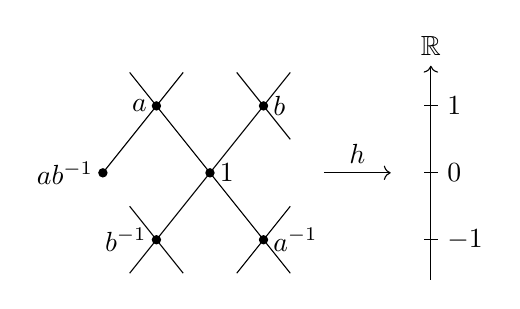
\begin{tikzpicture}[baseline=(current bounding box.center),scale=.85]
\draw (0,0)--(-.8,1) (0,0)--(.8,1) (0,0)--(-.8,-1) (0,0)--(.8,-1);
\draw (-.8,1)--(-1.6,0) (-.8,1)--(-1.2,1.5) (-.8,1)--(-.4,1.5);
\draw (.8,1)--(1.2,1.5) (.8,1)--(.4,1.5) (.8,1)--(1.2,.5);
\draw (-.8,-1)--(-1.2,-1.5) (-.8,-1)--(-.4,-1.5) (-.8,-1)--(-1.2,-.5);
\draw (.8,-1)--(1.2,-1.5) (.8,-1)--(.4,-1.5) (.8,-1)--(1.2,-.5);
\fill (0,0) circle (2pt) (-.8,1) circle (2pt) (.8,1) circle (2pt) (-.8,-1) circle (2pt) (.8,-1) circle (2pt) (-1.6,0) circle (2pt);
\node[right] at (0,0) {$1$};
\node[left] at (-.8,1) {$a$};
\node[right] at (.8,1) {$b$};
\node[left] at (-.8,-1) {$b^{-1}$};
\node[right] at (.8,-1) {$a^{-1}$};
\node[left] at (-1.6,0) {$ab^{-1}$};
\draw[->] (1.7,0)--node[above] {$h$}(2.7,0);
\draw[->] (3.3,-1.6)--(3.3,1.6) node[above] {$\mathbb{R}$};
\foreach \y in {-1,0,1} {\draw (3.2,\y)--(3.4,\y) node[right] {$\y$};}
\end{tikzpicture}
\]
The subcomplexes $X_i=h^{-1}([-i,i])$, for integers $i\geq 0$, form a $G$-invariant filtration of $X$.
Each quotient $G\backslash X_i$ is finite: its vertices are the integers from $-i$ to $i$, with two edges between consecutive integers.
However, the filtration is not essentially $0$-connected.
For any $j\geq 0$, choose an integer $m>j$.
The vertices $1$ and $a^mb^{-m}$ both lie in $X_0$, but their unique connecting path in the tree passes through $a^m$, of height $m$.
They therefore lie in different components of $X_j$.
By \autoref{thm:brown-finiteness}, $G$ is not of type $F_1$, that is, it is not finitely generated.
% Approved repair: height is defined on all words, and the two vertices give the failure of essential connectivity.
\end{example}

\subsection{Groups with exotic finiteness properties}
\label{subsec:exotic-finiteness}
We now construct two kinds of examples:
\begin{enumerate}
\item for each $n\geq 1$, a group $G_n$ of type $F_n$ but not of type $FP_{n+1}$;
\item a group $G$ of type $FP$ but not of type $F_2$.
\end{enumerate}
We obtain them from right-angled Artin groups associated to finite flag complexes.
For a nonempty finite flag complex $L$, write $A_L$ for the right-angled Artin group associated to its $1$-skeleton.
Let $\varphi:A_L\to\mathbb{Z}$ be the homomorphism sending every vertex generator to $1$.
\begin{definition}
\label{def:bestvina-brady-group}
Let $L$ be a nonempty finite flag complex.
The \emph{Bestvina--Brady group} associated to $L$ is
\[
H_L=\ker\bigl(\varphi:A_L\to\mathbb{Z}\bigr),
\qquad \varphi(s)=1
\]
for every vertex generator $s$.
\end{definition}
By definition, we have a short exact sequence
\[
1\to H_L\to A_L\xrightarrow{\varphi}\mathbb{Z}\to 1.
\]
The result we need is the main theorem of Bestvina and Brady~\cite{BB97}.
\begin{theorem}[Bestvina--Brady, 1997]
\label{thm:bestvina-brady-finiteness}
Let $L$ be a nonempty finite flag complex and let $n\geq 1$.
\begin{enumerate}
\item The group $H_L$ is of type $FP_n$ if and only if $L$ is $(n-1)$-acyclic over $\mathbb{Z}$, that is, $\widetilde H_i(L;\mathbb{Z})=0$ for $0\leq i\leq n-1$.
\item The group $H_L$ is of type $F_2$ if and only if $L$ is simply connected.
\item The group $H_L$ is of type $F_n$ if and only if $L$ is $(n-1)$-connected.
\end{enumerate}
\end{theorem}
% Approved clarification: L is nonempty and n>=1.
% Source: handwritten PDF, page 104.
\begin{proof}
We give only the idea of the proof, as in the notes.
Parts (1) and (2) use Morse theory.
Part (3) follows from them: for $n=1$, use $F_1\Leftrightarrow FP_1$; for $n\geq 2$, combine \autoref{thm:geometric-algebraic-finiteness} with \autoref{thm:hurewicz} to pass between $(n-1)$-acyclicity and $(n-1)$-connectivity in the simply connected case.
\end{proof}
\autoref{thm:bestvina-brady-finiteness} gives the first family.
\begin{example}
\label{ex:bestvina-brady-spheres}
Let $n\geq 1$ and give $S^n$ the flag triangulation
\[
L=(S^0)^{*(n+1)},
\]
the join of $n+1$ copies of the two-point complex $S^0$.
The sphere is $(n-1)$-connected but not $n$-acyclic, so $H_L$ is of type $F_n$ but not of type $FP_{n+1}$.
In this case,
\[
A_L=\prod_{i=1}^{n+1}\operatorname{Free}(2),
\qquad
H_L=\ker\left(\prod_{i=1}^{n+1}\operatorname{Free}(2)\xrightarrow{\varphi}\mathbb{Z}\right),
\]
where $\varphi$ sends all the indicated free generators to $1$.
% Approved correction: the sphere is a join of n+1 copies of S^0, and the product has n+1 factors.
\end{example}
For the second example, we use an acyclic space that is not simply connected.
\begin{example}
\label{ex:bestvina-brady-acyclic}
Let $L$ be a finite flag triangulation of the $2$-dimensional spine of the Poincar\'e homology sphere considered in \autoref{subsec:virtual-dimension}.
The complex $L$ is acyclic but not simply connected.
By \autoref{thm:bestvina-brady-finiteness}, $H_L$ is of type $FP_\infty$ but not of type $F_2$.
Since $H_L\leq A_L$ and the Salvetti complex gives a finite-dimensional model for $BA_L$, the group $H_L$ has finite cohomological dimension.
Thus \autoref{prop:fp-finite-dimension} shows that $H_L$ is of type $FP$.
Moreover, $\operatorname{cd}(H_L)=2$ by \cite[Examples~6.3(3)]{BB97}.
\end{example}
The following theorem is proved in \cite[Theorem~8.7]{BB97}.
\begin{theorem}[Bestvina--Brady]
Let $L$ be a finite flag triangulation of the $2$-dimensional spine of the Poincar\'e homology sphere.
Then $\operatorname{gd}(H_L)=3$ or the Whitehead asphericity conjecture, \autoref{conj:whitehead-asphericity}, is false.
\end{theorem}

% Editorial bibliography added during the reference audit on 2026-10-28.
\begin{thebibliography}{OAI26}
\bibitem[BB97]{BB97}
M.~Bestvina and N.~Brady,
\emph{Morse theory and finiteness properties of groups},
Invent. Math. \textbf{129} (1997), 445--470.
\href{https://doi.org/10.1007/s002220050168}{doi:10.1007/s002220050168}.

\bibitem[BLN01]{BLN01}
N.~Brady, I.~J.~Leary and B.~E.~A.~Nucinkis,
\emph{On algebraic and geometric dimensions for groups with torsion},
J. London Math. Soc. (2) \textbf{64} (2001), 489--500.
\href{https://doi.org/10.1112/S002461070100240X}{doi:10.1112/S002461070100240X}.

\bibitem[Bro82]{Bro82}
K.~S.~Brown,
\emph{Cohomology of Groups},
Graduate Texts in Mathematics, vol.~87, Springer, New York, 1982.
\href{https://doi.org/10.1007/978-1-4684-9327-6}{doi:10.1007/978-1-4684-9327-6}.

\bibitem[Bro87]{Bro87}
K.~S.~Brown,
\emph{Finiteness properties of groups},
J. Pure Appl. Algebra \textbf{44} (1987), 45--75.
\href{https://doi.org/10.1016/0022-4049(87)90015-6}{doi:10.1016/0022-4049(87)90015-6}.

\bibitem[Dav08]{Dav08}
M.~W.~Davis,
\emph{The Geometry and Topology of Coxeter Groups},
London Mathematical Society Monographs Series, vol.~32, Princeton University Press, Princeton, 2008.
\href{https://people.math.osu.edu/davis.12/davisbook.pdf}{Author's online version}.

\bibitem[Geo08]{Geo08}
R.~Geoghegan,
\emph{Topological Methods in Group Theory},
Graduate Texts in Mathematics, vol.~243, Springer, New York, 2008.
\href{https://doi.org/10.1007/978-0-387-74614-2}{doi:10.1007/978-0-387-74614-2}.

\bibitem[GR62]{GR62}
M.~Gerstenhaber and O.~S.~Rothaus,
\emph{The solution of sets of equations in groups},
Proc. Natl. Acad. Sci. USA \textbf{48} (1962), 1531--1533.
\href{https://doi.org/10.1073/pnas.48.9.1531}{doi:10.1073/pnas.48.9.1531}.

\bibitem[Hat02]{Hat02}
A.~Hatcher,
\emph{Algebraic Topology},
Cambridge University Press, Cambridge, 2002.
\href{https://pi.math.cornell.edu/~hatcher/AT/ATpage.html}{Author's online version}.

\bibitem[Luc00]{Luc00}
W.~L\"uck,
\emph{The type of the classifying space for a family of subgroups},
J. Pure Appl. Algebra \textbf{149} (2000), 177--203.
\href{https://doi.org/10.1016/S0022-4049(98)90173-6}{doi:10.1016/S0022-4049(98)90173-6}.

\bibitem[OAI26]{OAI26}
OpenAI,
\emph{A finitely generated counterexample to the Eilenberg--Ganea conjecture},
preprint, September 23, 2026.
\href{https://github.com/openai/math/blob/main/preprints/A-finitely-generated-counterexample-to-the-Eilenberg-Ganea-conjecture-September-23-2026/paper.pdf}{Preprint}.

\end{thebibliography}
\end{document}
